\section{System Design}   
    The festival prioritises a minimum \gls{spl} of \SI{96}{\decibel} at \gls{foh} for optimal mixing while actively addressing noise pollution concerns in nearby areas. Ensuring even coverage across the venue is essential, and strict adherence to regulations is maintained.

    The design incorporates specified d\&b Audiotechnik products, covering calculations for delay times, rigging, power requirements, amp configurations, and routing. Relevant \gls{spl} maps for the festival area are also provided, utilising software such as d\&b ArrayCalc, d\&b NoizCalc, and d\&b R1. Additionally, SubAligner and Excel were employed for calculating delay compensations and power consumption.
    
    \subsection{System Overview}
    The \gls{isl} \eqref{eq:inverse_square_law} can be used to estimate the \gls{spl} by considering the uniform emission of sound from a point source in all directions \citep{wkc2023}.

    \begin{equation}\label{eq:inverse_square_law}
        Lp(R2) = Lp(R1) - 20 \cdot \log_{10}\left(\frac{R2}{R1}\right)
    \end{equation}
        
    Where:
    \begin{itemize}
        \item $Lp(R1)$ is the known sound pressure level at the first location (typically measured data or equipment vendor data).
        \item $Lp(R2)$ is the unknown sound pressure level at the second location.
        \item $R1$ is the distance from the noise source to the location of the known sound pressure level.
        \item $R2$ is the distance from the noise source to the second location.
    \end{itemize}

    However, line arrays defeat the \gls{isl} with a \SI{-3}{\decibel} drop per distance doubling \citep{brown2010} \eqref{eq:modified_inverse_square_law} however, in a practical scenario this is not always the case, and only continues up to a certain distance \citep{dstewart2016}. A line array directs constructive interference to the center and induces destructive interference at the sides, enhancing projection towards the audience while minimising reflection from the floor and ceiling \citep{dmellor2006}.

    \begin{equation}\label{eq:modified_inverse_square_law}
        Lp(R2) = Lp(R1) - 10 \cdot \log_{10}\left(\frac{R2}{R1}\right)
    \end{equation}

    From this the number of speakers needed in a line array can be calculated by considering the superposition principle of sound waves \eqref{eq:summation_of_speakers}. Where the power of two sources are the same, when stacked adds approximately \SI{3.01}{\decibel}.

    \begin{equation}\label{eq:summation_of_speakers}
        \text{Total dB} = 10 \cdot \log_{10}\left(\sum_{i=1}^{n} 10^{(a_i/10)}\right)
    \end{equation}

    Using this, 22 flown GSL12 speakers was calculated for the main array and 18 KSL12 speakers for the delay per side. As well as 12 SL-Subs on the ground for \gls{foh} and 4 flown KSL-Subs for the delay.
    
    ArrayCalc simplifies system optimisation by including a CUT button to eliminate lower frequencies, reducing interference with subs and improving amplifier efficiency. The tool also features \gls{hfa} for natural frequency response, 'line' and 'arc' options for speaker settings, and a \gls{cpl} attenuation function to address near field effects in straight array sections and Array Processing for advanced system tuning. All of which are explored in the system design.

    Subwoofers have cardioid and omni-directional patterns for directing low frequencies. Passive systems are suitable for larger venues, offering greater power and easy amplifier access when flown, unlike active subs which lack power. Therefore, passive systems are used in this design.

    The directivity rule is crucial in subwoofer arrays. Lower frequencies are omni-directional, so array layouts focus on efficient sound direction.
    Techniques include beam-forming for polar pattern shaping, gain shading for regular coverage \citep{jberryman2010}, and three main subwoofer array types: 
    
    \begin{itemize}
        \item \textbf{Broadside} common and versatile, with variations like straight, curved, or stair-cased rows affecting polar patterns.
        \item \textbf{Gradient} uses amplitude and phase variations for even lower frequency distribution, common in outdoor venues for maintaining sound levels over long distances.
        \item \textbf{End-fire} lines of speakers pointing in the desired direction with set delay times, effective with a larger number of speakers.
    \end{itemize}

    The main array will be flown as this improves energy distribution and reduces SPL excess in the front. However, the sub array will be ground stacked as they offer an extra 6dB in sub frequencies through coupling with the ground. A gradient array with broadside characteristics will be used to create a cardioid pattern.The J series was not chosen as they are now discontinued.

    \begin{longtable}[H]{|l|p{7cm}|p{7cm}|}
        \hline
        Series & Description & Advantages \\ \hline
        \endfirsthead
        %
        \endhead
        %
        GSL & Large scale applications. & Precision and power for large events. Exceptional directivity and coverage control. Optimized for stadium and festival environments. \\ \hline
        KSL & Medium to large scale applications. & High-performance system with extended low-frequency response. Versatile rigging options for easy integration into various venues. \\ \hline
        J-Series & Versatile for both small and large-scale applications. & Exceptional audio quality with flexible configurations. Versatility in system design, suitable for both permanent installations and touring applications. \\ \hline
        \caption{Comparison of d\&b line array series}
        \label{tab:db_series_comparison}
    \end{longtable}

    \begin{figure}[H]
        \centering
        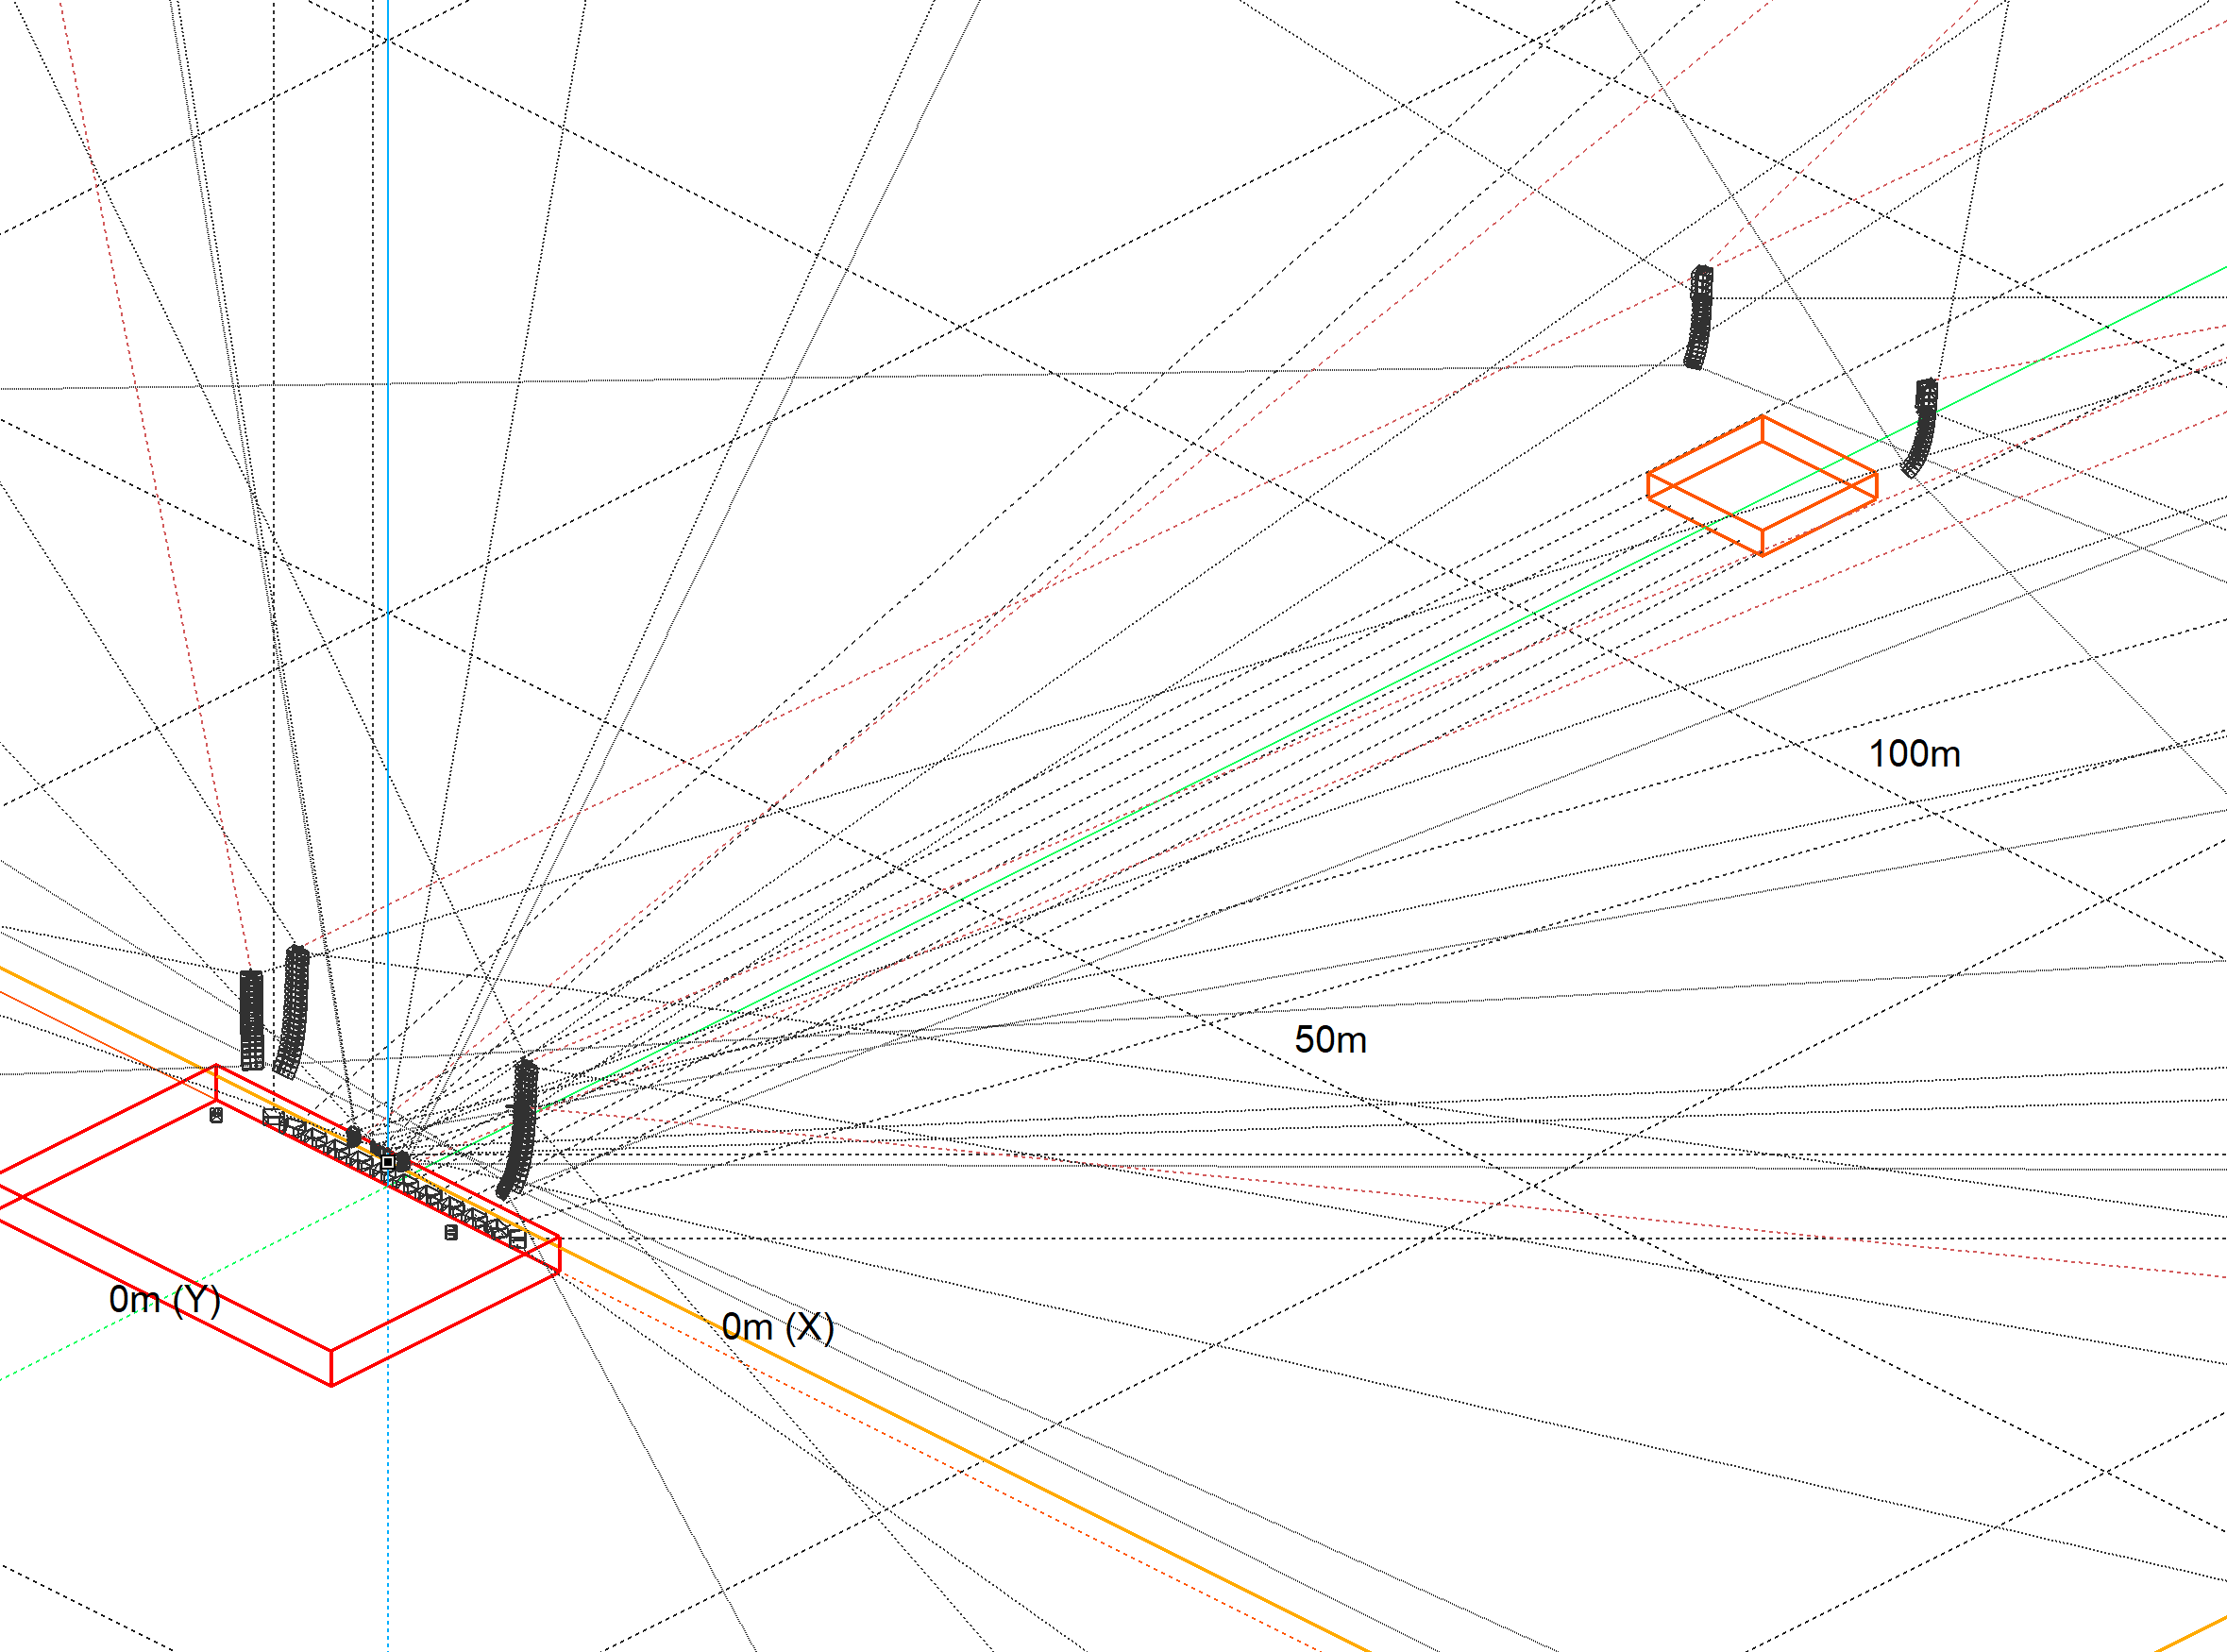
\includegraphics[width=1\linewidth]{Images/full_system.png}
        \caption{Full System}
        \label{fig:full_system}
    \end{figure}
    
    \subsubsection{Parts List}
        The complete parts list is located at \ref{appendix:speaker_parts}.

    \subsubsection{Rigging Requirements}
        The full rigging requirements are provided at \ref{appendix:speaker_rigging} with the required pick points, loads and dimensions specified.

    \subsubsection{Delay Times}
        Delays are crucial to ensure proper alignment of multiple audio sources. Especially when arrays are distributed across different locations and distances from the audience. To calculate the necessary delay times for each speaker array, trigonometry is employed to account for the varying distances between the individual speaker hangs.

        The time delay ($t$) needed to time-align two speaker systems with positions ($x_1, y_1, z_1$) and ($x_2, y_2, z_2$) can be calculated using the formula \eqref{eq:time_delay}:

        \begin{equation}\label{eq:time_delay}
            t = \frac{\sqrt{(x_2 - x_1)^2 + (y_2 - y_1)^2 + (z_2 - z_1)^2}}{v}
        \end{equation}

        where ($v$) is the speed of sound in air.

        To calculate the speed of sound ($v$), the following formula is used \eqref{eq:speed_of_sound}:

        \begin{equation}\label{eq:speed_of_sound}
            v = 331.4 \sqrt{1 + \frac{T}{273.15}} + 0.6 \times H
        \end{equation}

        where ($T$) is the temperature in degrees Celsius, and ($H$) is the relative humidity.
        
        \citet{cramer1993} demonstrates equations that includes the altitude \eqref{eq:complex_speed_of_sound}. Using the altitude value, the air pressure is calculated with the barometric formula \eqref{eq:barometric_formula}:

        \begin{equation}\label{eq:barometric_formula}
            P = P_0 e^{-\frac{gM(h - h_0)}{RT}}
        \end{equation}
            
        Where:
        \begin{itemize}
            \item $h$ is the altitude at which we want to calculate the pressure, expressed in meters.
            \item $P$ is the air pressure at altitude $h$.
            \item $P_0$ is the pressure at the reference level $h_0$. In our pressure calculator, it is assumed that the reference level is located as sea level, so $h_0 = 0$.
            \item $T$ is the temperature at altitude $h$, expressed in Kelvins. The temperature at altitude calculator may help you find it.
            \item $g$ is the acceleration due to the gravitational force. For Earth, $g = \SI{9.80665}{\m/s\squared}$.
            \item $M$ is the molar mass of air. For Earthly air, $M = \SI{0.0289644}{\kg\mol}$.
            \item $R$ is the universal gas constant. Its value is equal to $R = \SI{8.31432}{N \cdot m/(mol \cdot K)}$.
        \end{itemize}

        This is then applied to \citeauthor{cramer1993}'s formula \eqref{eq:complex_speed_of_sound}:

        \begin{equation}\label{eq:complex_speed_of_sound}
            \begin{aligned}
            ENH &= \pi \cdot 10^{-8}P + 1.00062 + T^2 \cdot 5.6 \cdot 10^{-7} \\
            PSV_1 &= T_k^2 \cdot 1.2378847 \cdot 10^{-5} - 1.9121316 \cdot 10^{-2} \cdot T_k \\
            PSV_2 &= 33.93711047 - 6.3431645 \cdot 10^3 / T_k \\
            PSV &= e^{PSV_1} \cdot e^{PSV_2} \\
            H &= Rh \cdot ENH \cdot \frac{PSV}{P} \\
            X_w &= \frac{H}{100} \\
            X_c &= 400 \cdot 10^{-6} \\
            C_1 &= 0.603055T + 331.5024 - T^2 \cdot 5.28 \cdot 10^{-4} + \\ & \ldots (0.1495874T + 51.471935 - T^2 \cdot 7.82 \cdot 10^{-4}) \cdot X_w \\
            C_2 &= (-1.82 \cdot 10^{-7} + 3.73 \cdot 10^{-8}T - T^2 \cdot 2.93 \cdot 10^{-10})P + \\ & \ldots (-85.20931 - 0.228525T + T^2 \cdot 5.91 \cdot 10^{-5})X_c \\
            C_3 &= X_w^2 \cdot 2.835149 + P^2 \cdot 2.15 \cdot 10^{-13} - X_c^2 \cdot 29.179762 - 4.86 \cdot 10^{-4}X_wPX_c \\
            C &= C_1 + C_2 - C_3
            \end{aligned}
        \end{equation}

        Where:
        \begin{itemize}
            \item $Rh$: is the relative humidity.
            \item $Tk$: is the measured ambient temperature in kelvins.
            \item $ENH$: is the molecular concentration of water vapour calculated from $Rh$. Using Giacomo's methods as demonstrated by \citeauthor{rasmussen1997}.
            \item $PSV$ values: are constants taken from \citeauthor{cramer1993}'s equations.
            \item $H$: is the molecular concentration of water vapour.
            \item $Xw$: is the mole fraction of carbon dioxide and water vapour, respectively.
            \item $C$ values: are the speed calculated using the method of \citeauthor{cramer1993} from JASA vol 93 page 2510
        \end{itemize}
        
        Referring to weather averages for Newcastle in July, the temperature typically ranges between 19°C and 13°C, with humidity averaging around 75\% \citep{worldweatheronline2023}.

        Table \ref{tab:delay_times} displays the approximate delay compensations for each source, where the delay reference point is at $X=\SI{150}{\metre}, Y=\SI{0}{\metre}$. These may differ to the ArrayCalc times as phase is also considered to closely align with the subs at specific frequencies as shown in Figure \ref{fig:delay_alignment}. The supporting calculations are provided in the 'DelayAlignTimes' excel file.

        \begin{longtable}[c]{|lllll|}
            \hline
            \multicolumn{5}{|l|}{Temperature = \SI{16}{\celsius}, Humidity = 75\%, Altitude = \SI{64}{\metre}} \\ \hline
            \endfirsthead
            %
            \endhead
            %
            \multicolumn{1}{|l|}{\textbf{Source}} & \multicolumn{1}{l|}{\textbf{X}} & \multicolumn{1}{l|}{\textbf{Y}} & \multicolumn{1}{l|}{\textbf{Z}} & \textbf{Total Delay} \\ \hline
            \multicolumn{1}{|l|}{Delay} & \multicolumn{1}{l|}{\SI{125}{\metre}} & \multicolumn{1}{l|}{\SI{10}{\metre}} & \multicolumn{1}{l|}{\SI{10.5}{\metre}} & \multicolumn{1}{l|}{\SI{364.39}{\ms}} \\ \hline
            \multicolumn{1}{|l|}{Main} & \multicolumn{1}{l|}{\SI{2.4}{\metre}} & \multicolumn{1}{l|}{\SI{10}{\metre}} & \multicolumn{1}{l|}{\SI{12}{\metre}} & \multicolumn{1}{l|}{\SI{13.34}{\ms}} \\ \hline
            \multicolumn{1}{|l|}{Outfill} & \multicolumn{1}{l|}{\SI{0}{\metre}} & \multicolumn{1}{l|}{\SI{12}{\metre}} & \multicolumn{1}{l|}{\SI{10.5}{\metre}} & \multicolumn{1}{l|}{\SI{6.20}{\ms}} \\ \hline
            \multicolumn{1}{|l|}{Sub} & \multicolumn{1}{l|}{\SI{0}{\metre}} & \multicolumn{1}{l|}{\SI{0}{\metre}} & \multicolumn{1}{l|}{\SI{0}{\metre}} & \multicolumn{1}{l|}{\SI{8.33}{\ms}} \\ \hline
            \multicolumn{1}{|l|}{Nearfill} & \multicolumn{1}{l|}{\SI{-0.6}{\metre}} & \multicolumn{1}{l|}{\SI{2.20}{\metre}} & \multicolumn{1}{l|}{\SI{2.5}{\metre}} & \multicolumn{1}{l|}{\SI{6.55}{\ms}} \\ \hline
            \multicolumn{1}{|l|}{Frontfill} & \multicolumn{1}{l|}{\SI{0}{\metre}} & \multicolumn{1}{l|}{\SI{0}{\metre}} & \multicolumn{1}{l|}{\SI{0}{\metre}} & \multicolumn{1}{l|}{\SI{8.33}{\ms}} \\ \hline

            \caption{Delay Times}
            \label{tab:delay_times}
        \end{longtable}

        \begin{figure}[H]
            \centering
            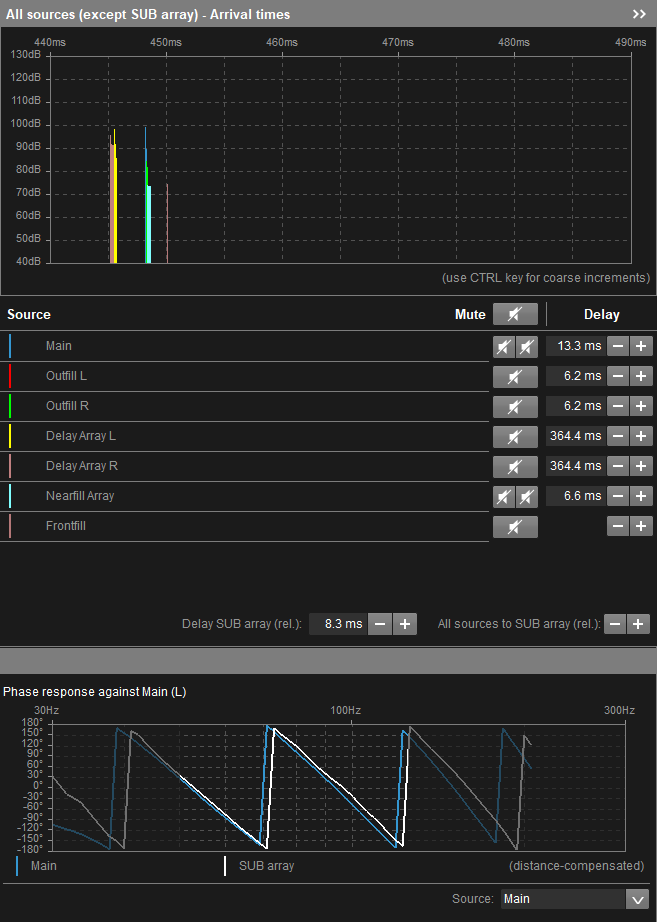
\includegraphics{Images/delay_alignment.png}
            \caption{Time and phase alignment of sources}
            \label{fig:delay_alignment}
        \end{figure}

        All delay times are written in full at \ref{appendix:speaker_delays}.
        
    \subsubsection{SPL Mapping}
     The \gls{spl} mapping of the system can be seen in Table \ref{tab:spl_mapping}; showing the highest, lowest, standard deviation and average \gls{spl}.
     
        \begin{longtable}[H]{|c|c|c|c|c|c|}
            \hline
            \multicolumn{1}{|c|}{\textbf{Freq}} &
            \multicolumn{1}{c|}{\textbf{Screenshot}} &
            \multicolumn{1}{c|}{\textbf{\begin{tabular}[c]{@{}c@{}}High\\ SPL\end{tabular}}} &
            \multicolumn{1}{c|}{\textbf{\begin{tabular}[c]{@{}c@{}}Low\\ SPL\end{tabular}}} &
            \multicolumn{1}{c|}{\textbf{\begin{tabular}[c]{@{}c@{}}Std\\ Dev\end{tabular}}} &
            \textbf{\begin{tabular}[c]{@{}c@{}}Avg.\\ SPL\end{tabular}} \\ \hline
            \endfirsthead
            %
            \endhead
            %
            \multicolumn{6}{|c|}{\textbf{Sub Array Only (all other sources muted)}}                                                                           \\ \hline
            \multicolumn{1}{|c|}{\SI{50}{\Hz}}  & \multicolumn{1}{c|}{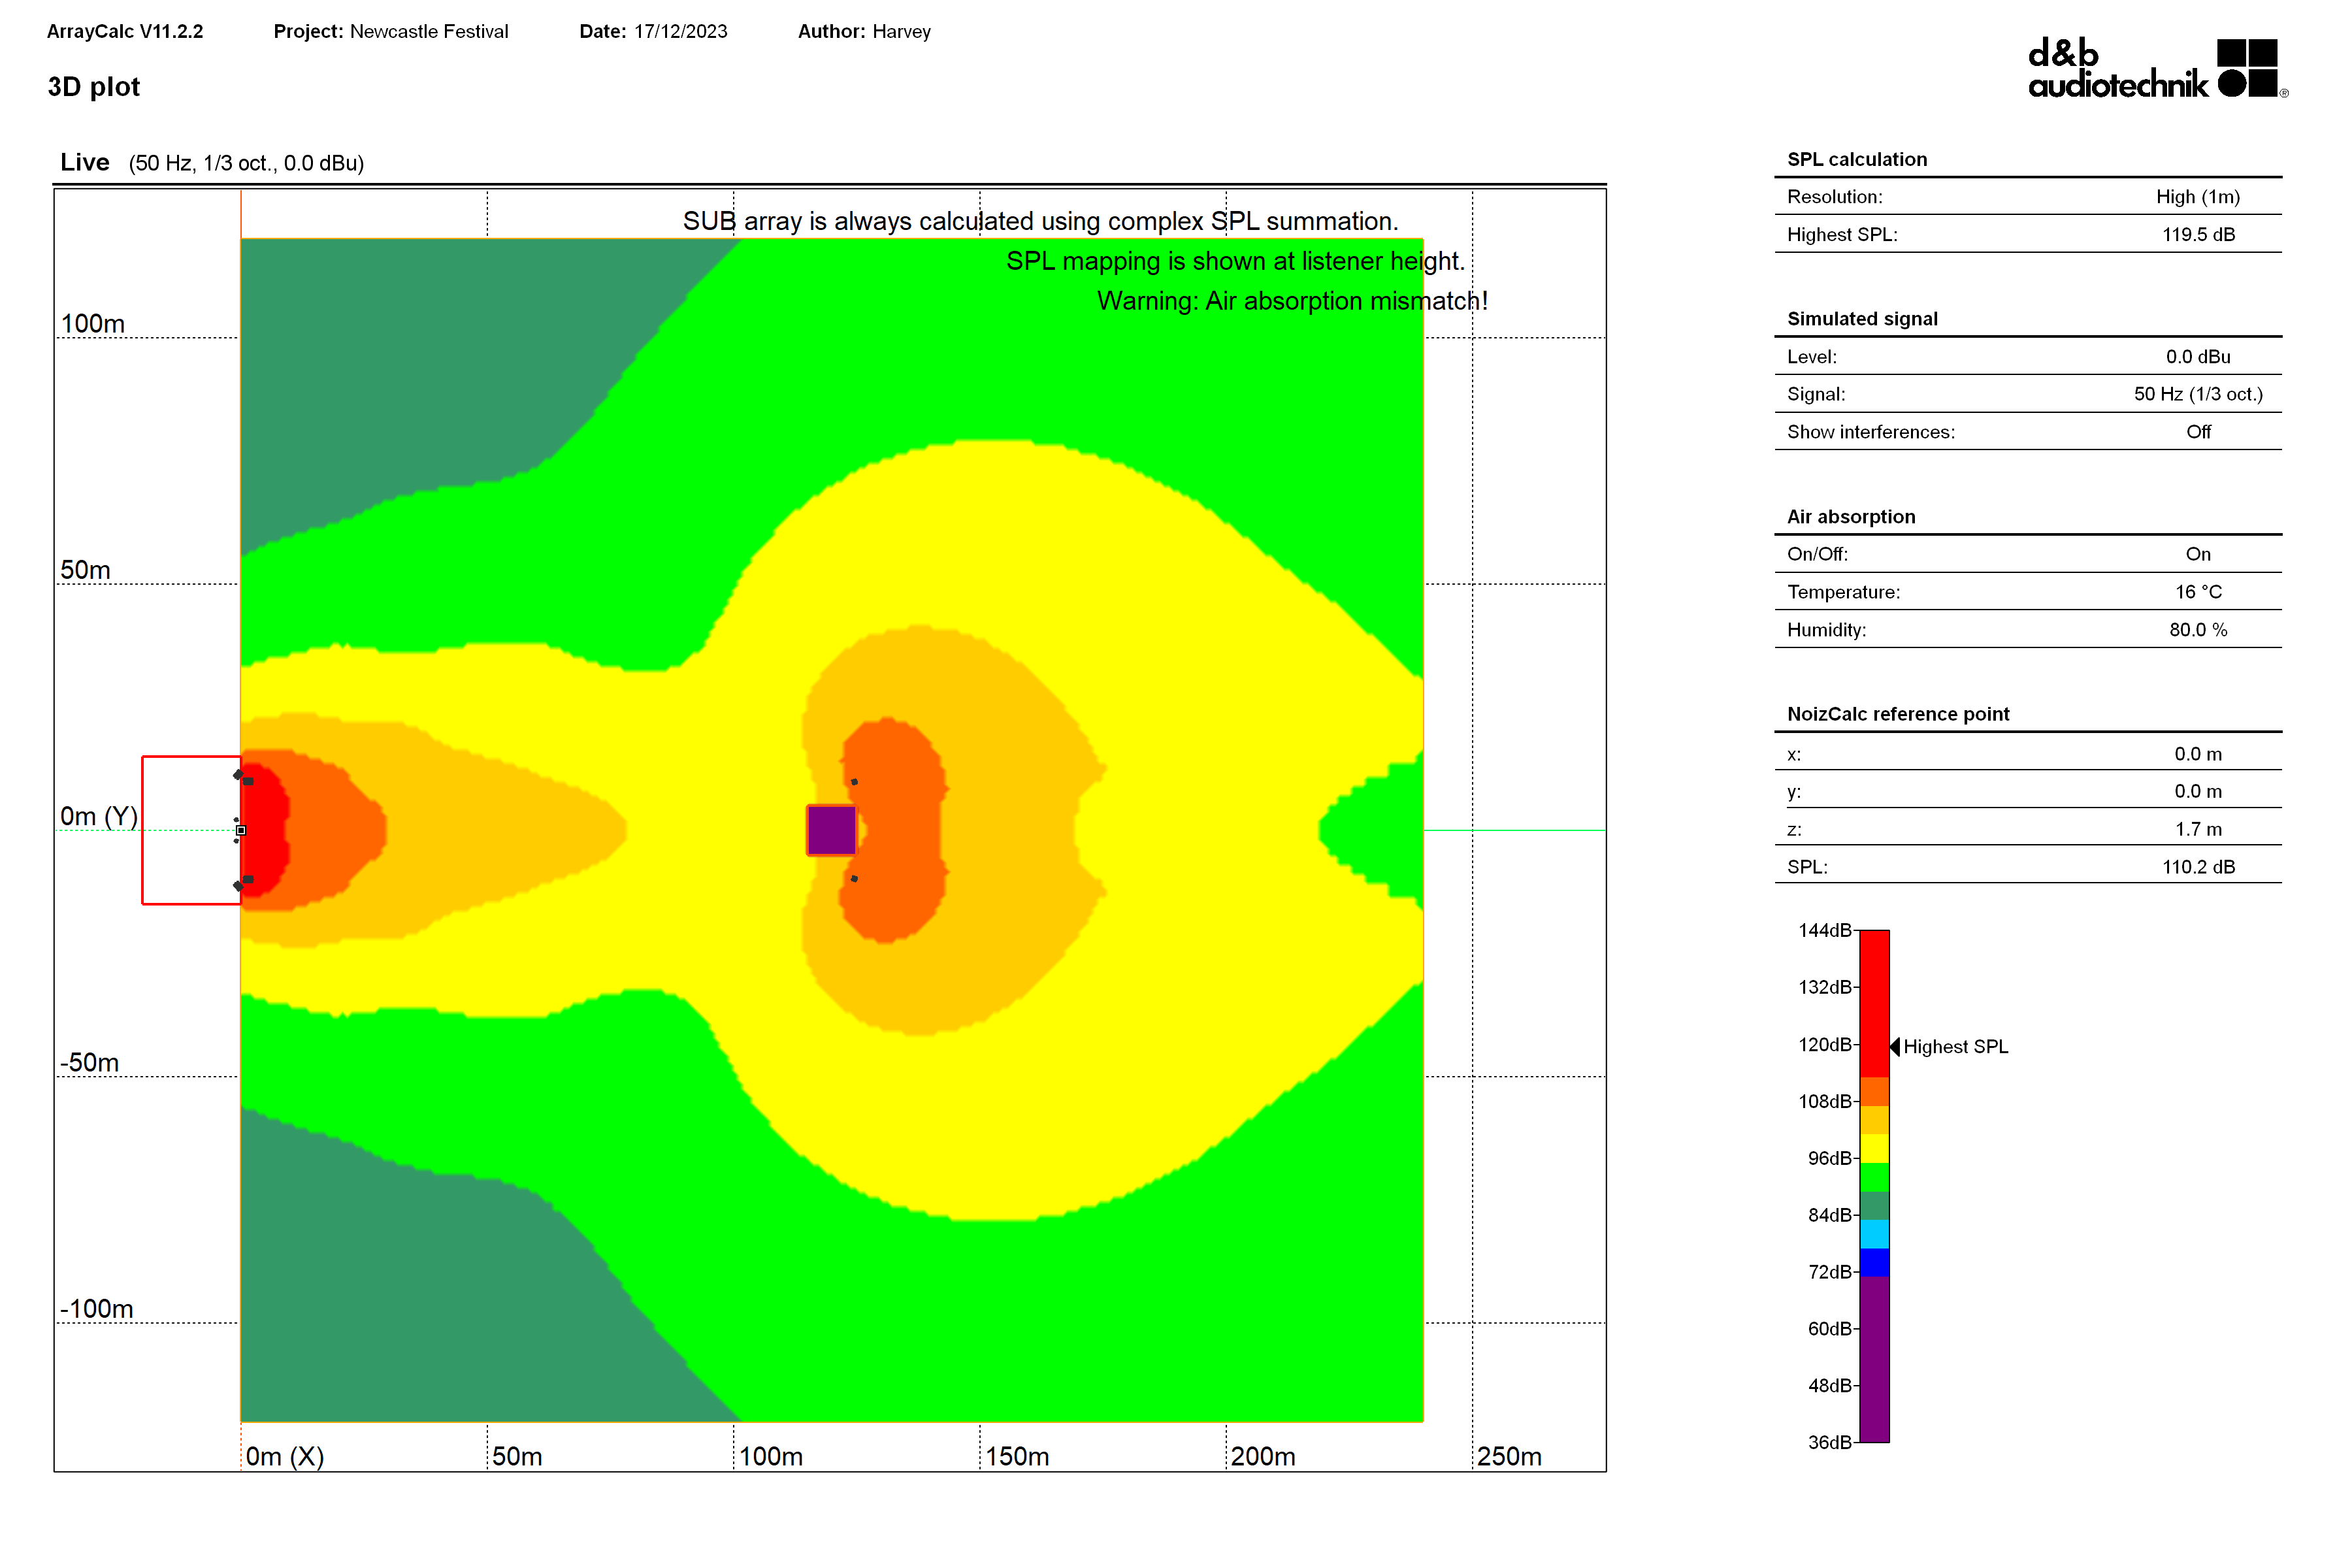
\includegraphics[width=0.5\textwidth]{Images/spl_plot_50hz_subs.png}}  & \multicolumn{1}{c|}{\SI{119.5}{\dB}} & \multicolumn{1}{c|}{\SI{84}{\dB}}  & \multicolumn{1}{c|}{\SI{25.1}{\dB}} & \SI{101.8}{\dB} \\ \hline
            \multicolumn{1}{|c|}{\SI{100}{\Hz}} & \multicolumn{1}{c|}{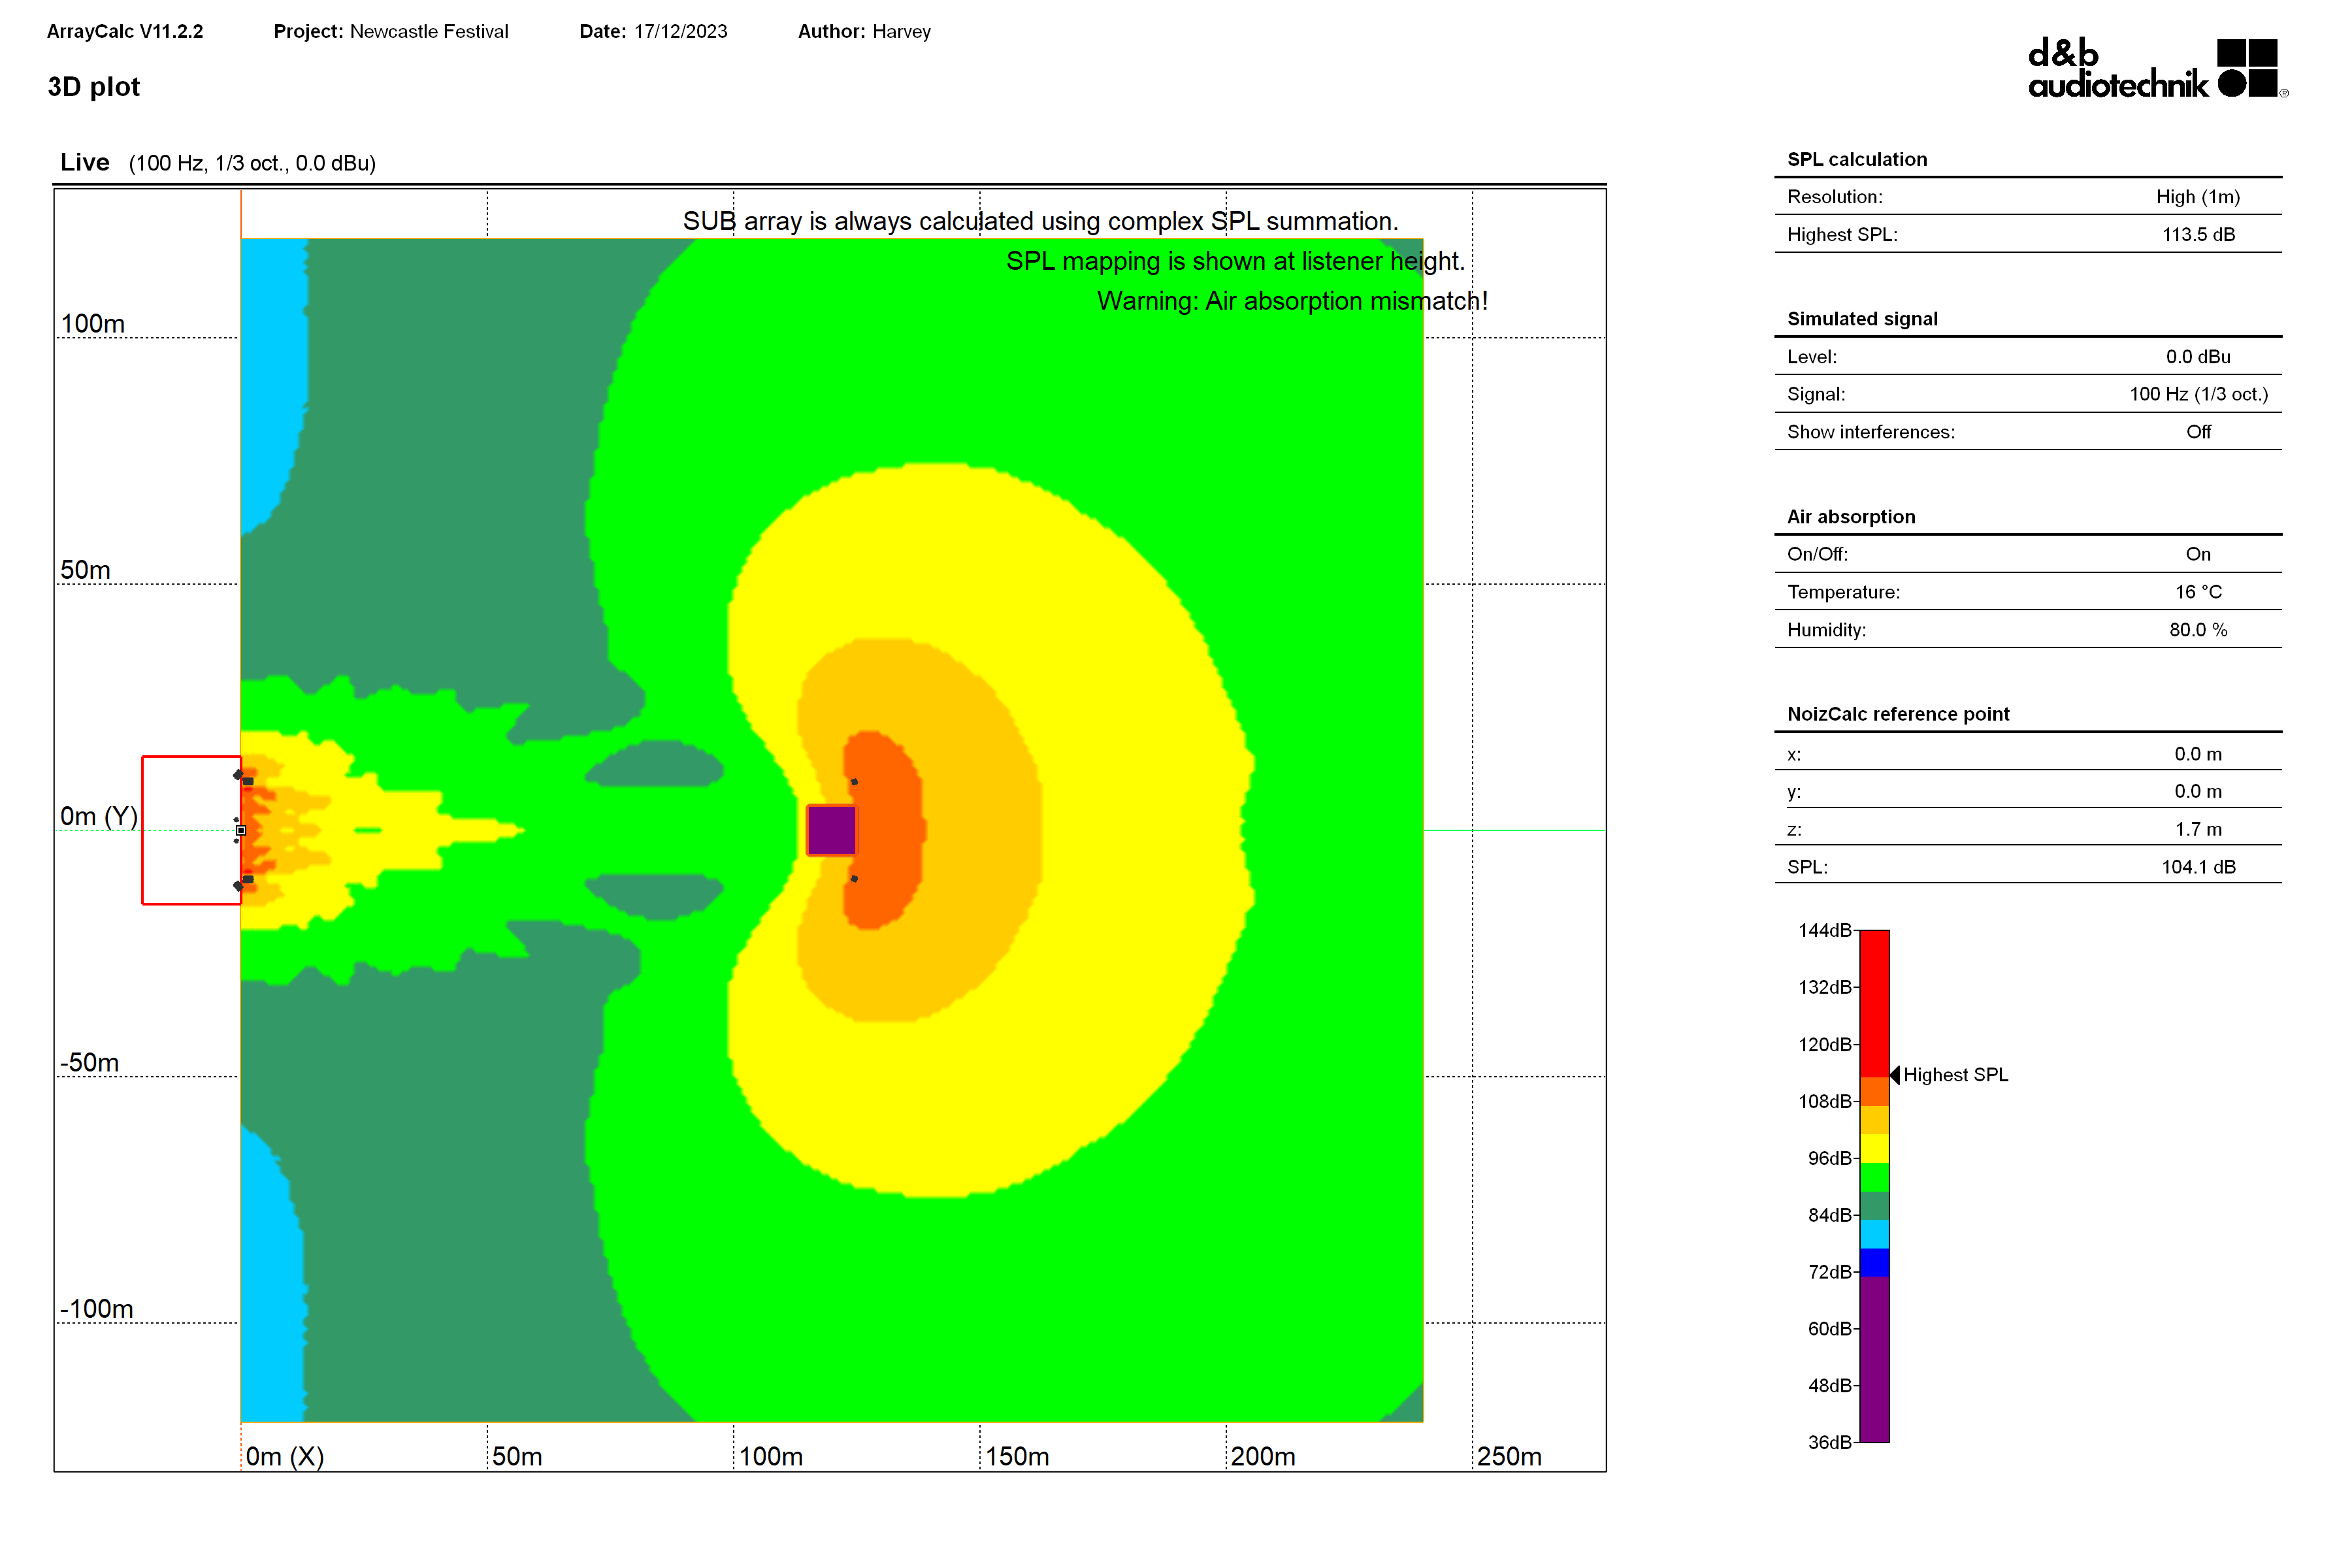
\includegraphics[width=0.5\textwidth]{Images/spl_plot_100hz_subs.png}} & \multicolumn{1}{c|}{\SI{113.5}{\dB}} & \multicolumn{1}{c|}{\SI{78}{\dB}}  & \multicolumn{1}{c|}{\SI{25.1}{\dB}} & \SI{95.8}{\dB} \\ \hline
            \multicolumn{6}{|c|}{\textbf{Full System}}                                                                                                        \\ \hline
            \multicolumn{1}{|c|}{\SI{50}{\Hz}}  & \multicolumn{1}{c|}{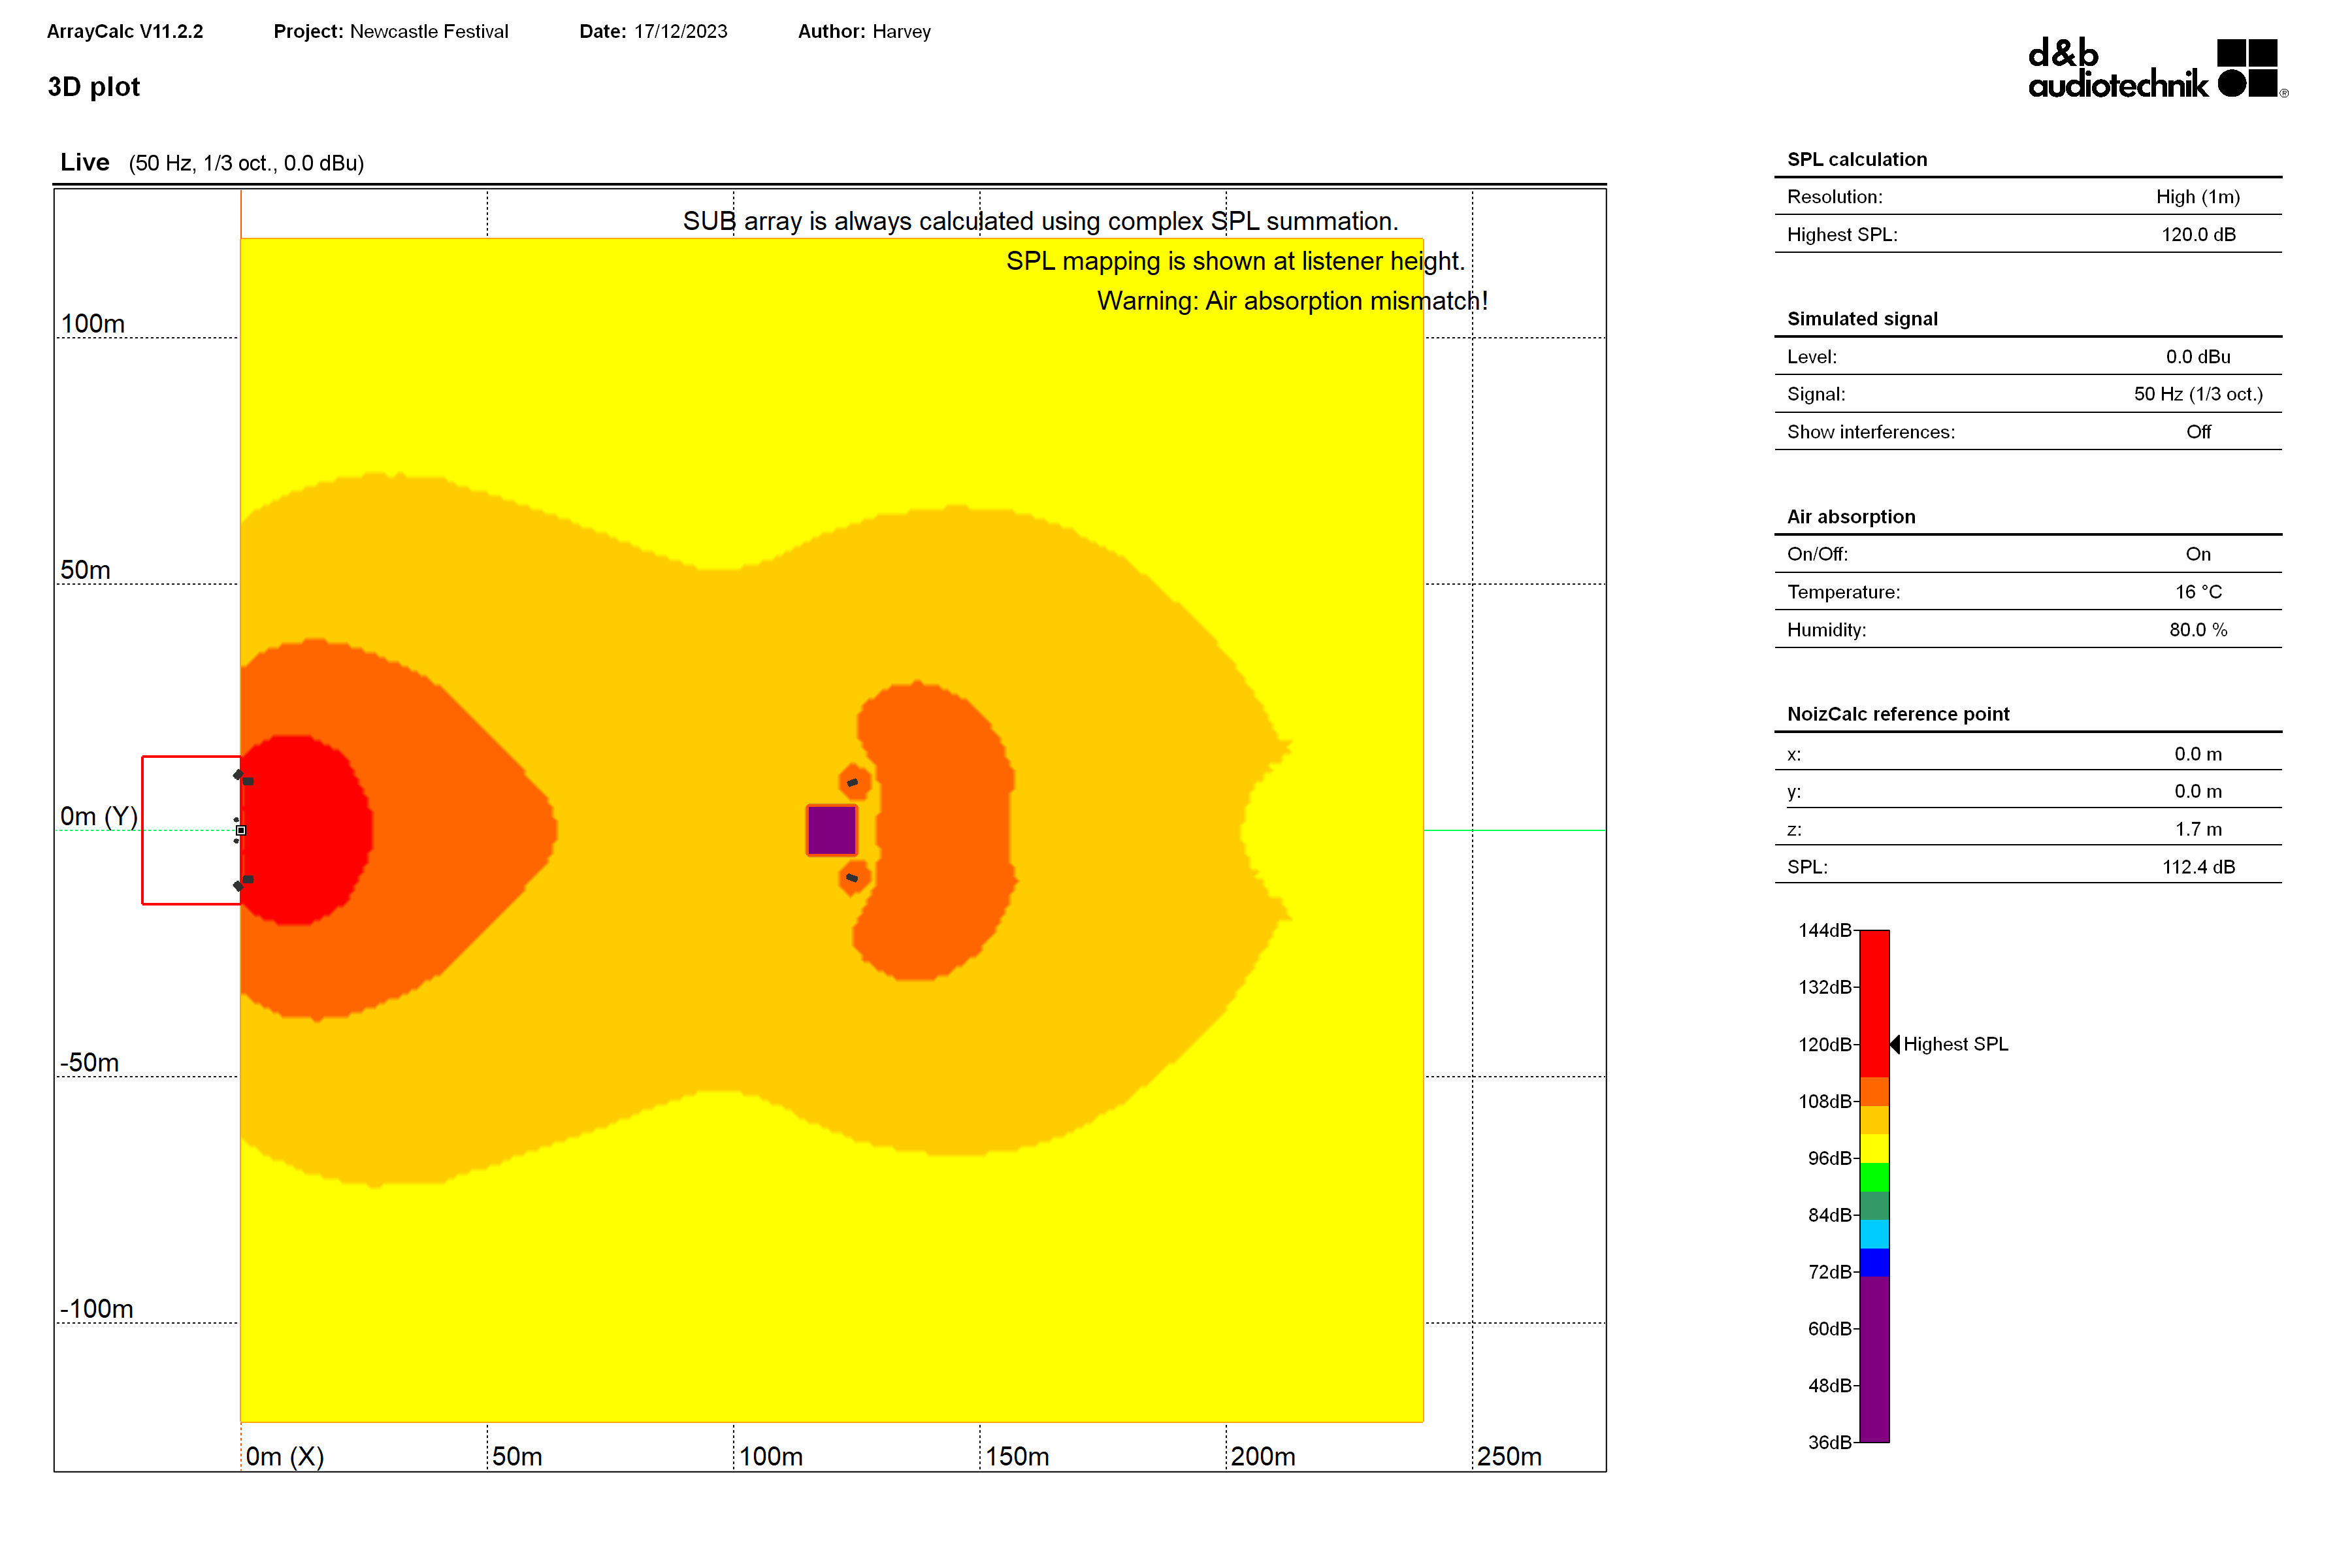
\includegraphics[width=0.5\textwidth]{Images/spl_plot_50hz_all.png}}   & \multicolumn{1}{c|}{\SI{120.0}{\dB}} & \multicolumn{1}{c|}{\SI{96}{\dB}}  & \multicolumn{1}{c|}{\SI{17.0}{\dB}} & \SI{108.0}{\dB} \\ \hline
            \multicolumn{1}{|c|}{\SI{100}{\Hz}} & \multicolumn{1}{c|}{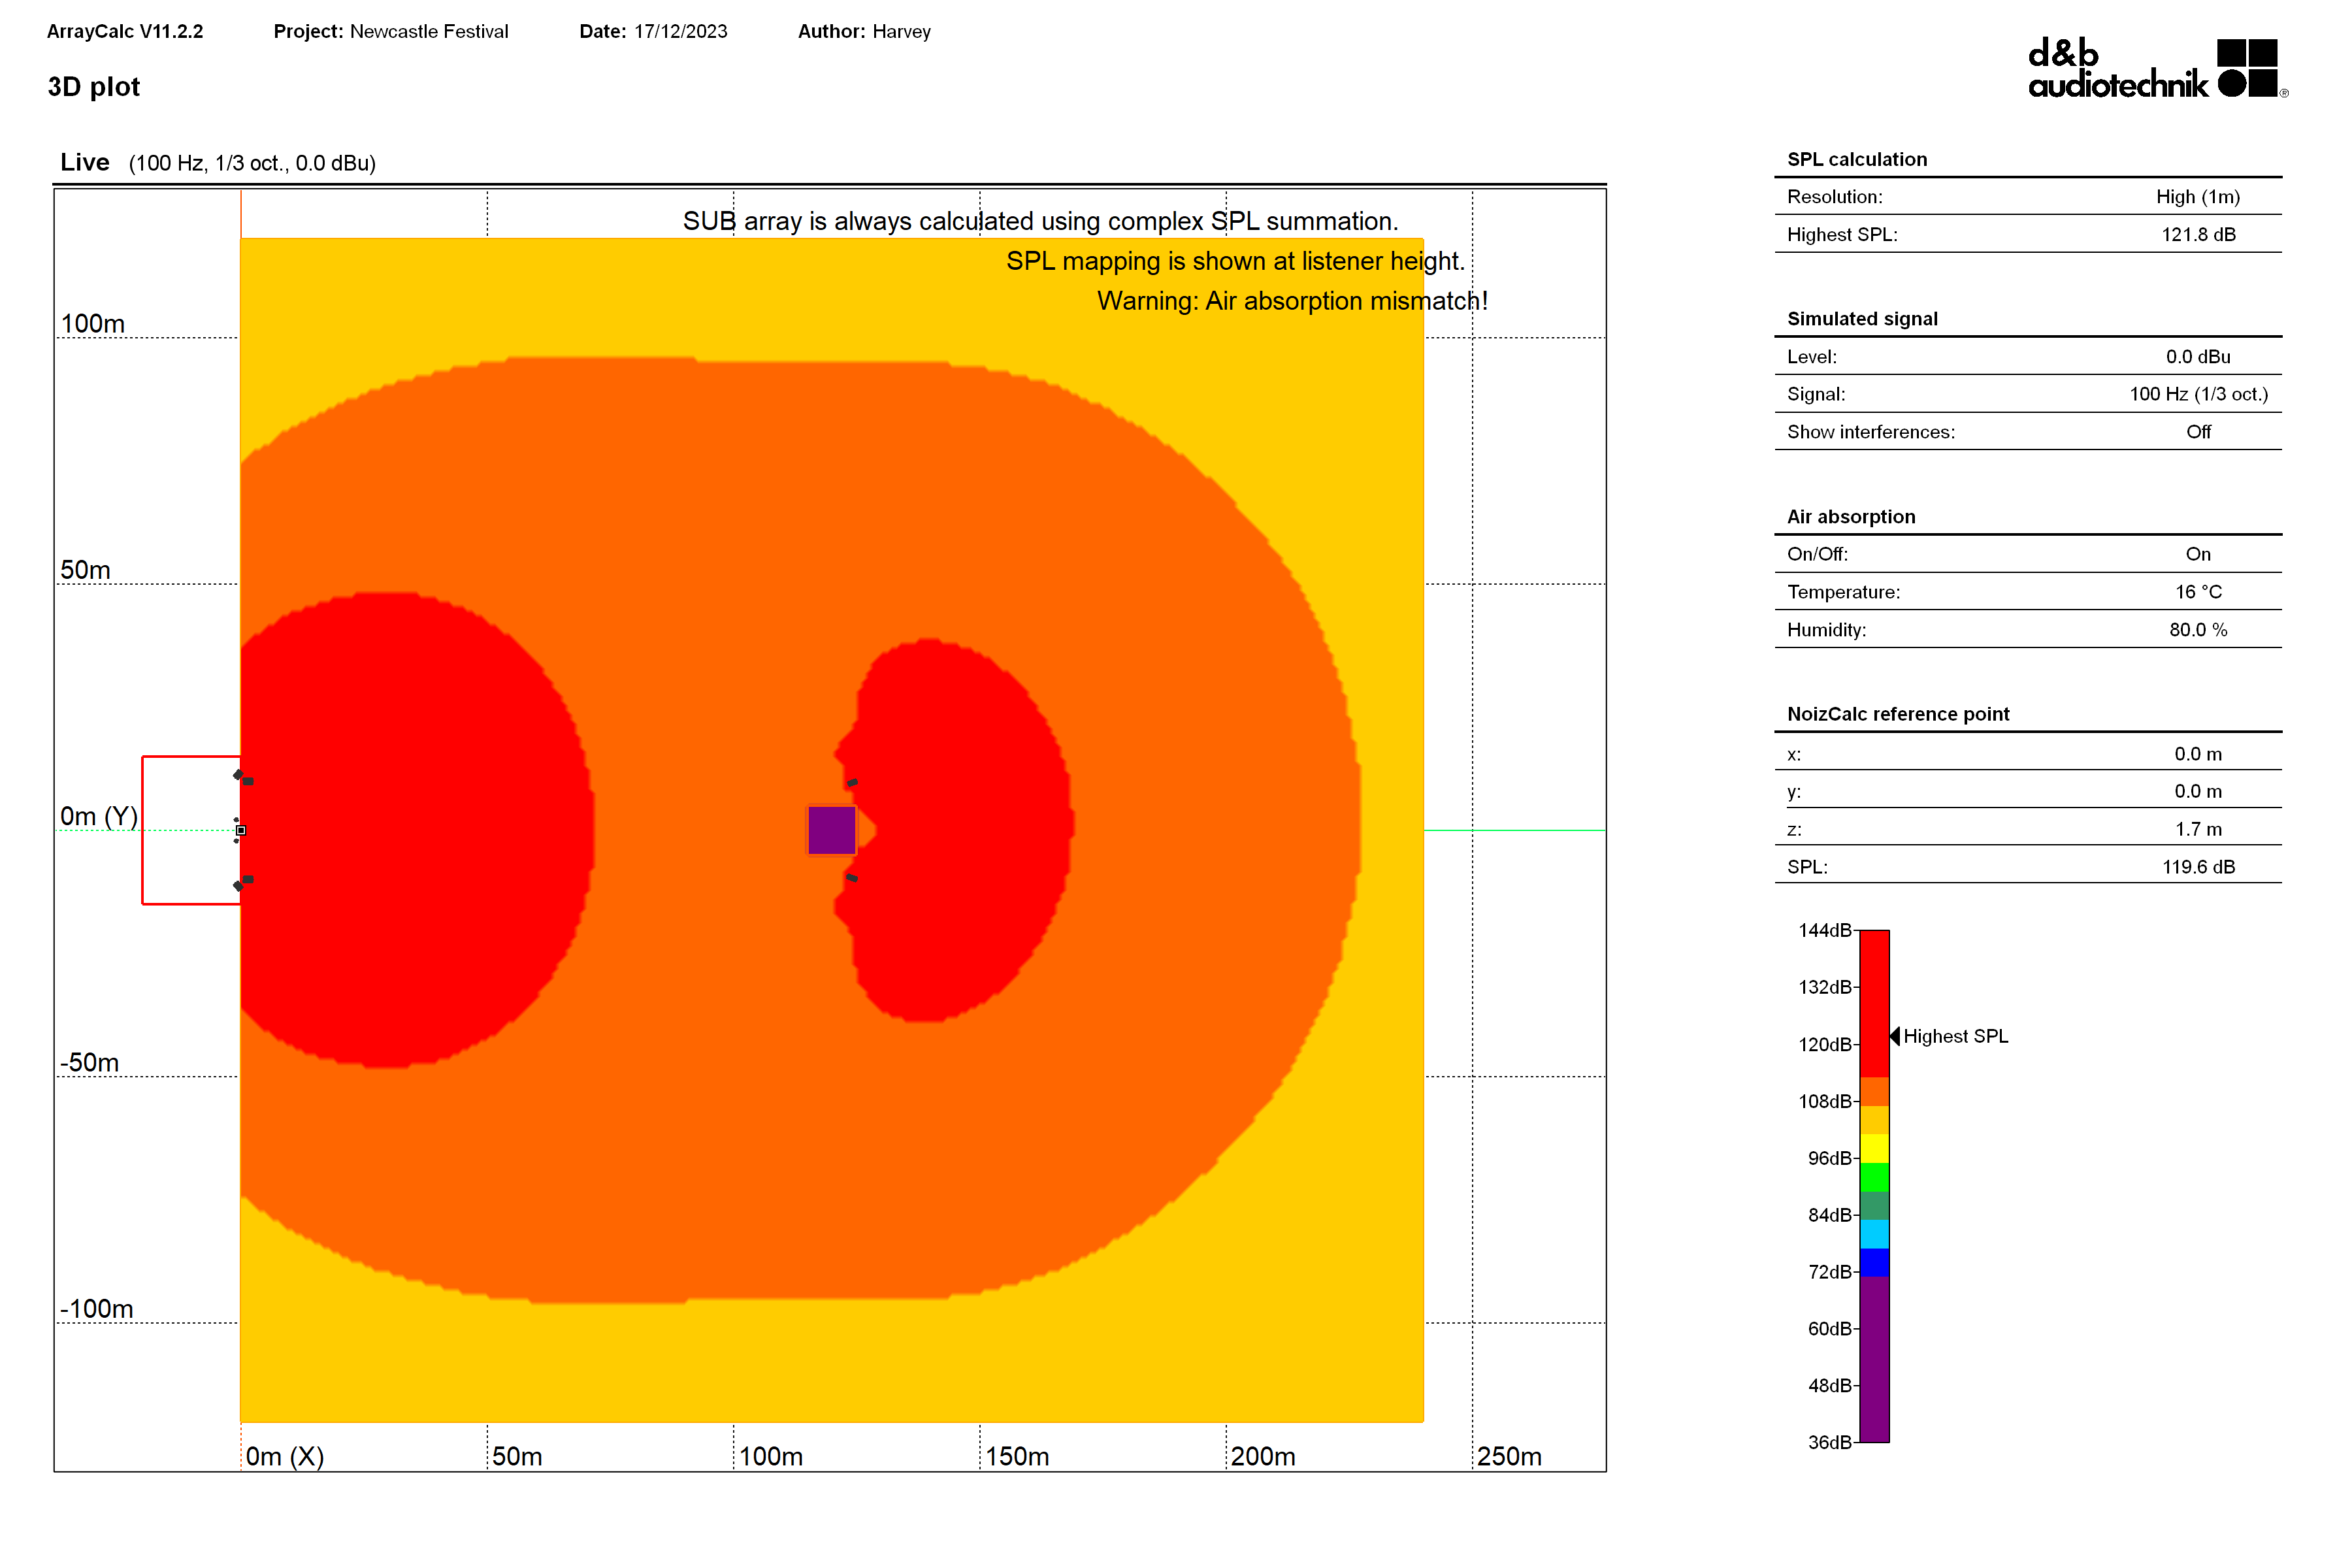
\includegraphics[width=0.5\textwidth]{Images/spl_plot_100hz_all.png}}  & \multicolumn{1}{c|}{\SI{121.8}{\dB}} & \multicolumn{1}{c|}{\SI{102}{\dB}} & \multicolumn{1}{c|}{\SI{14.0}{\dB}} & \SI{111.9}{\dB} \\ \hline
            \multicolumn{1}{|c|}{\SI{500}{\Hz}} & \multicolumn{1}{c|}{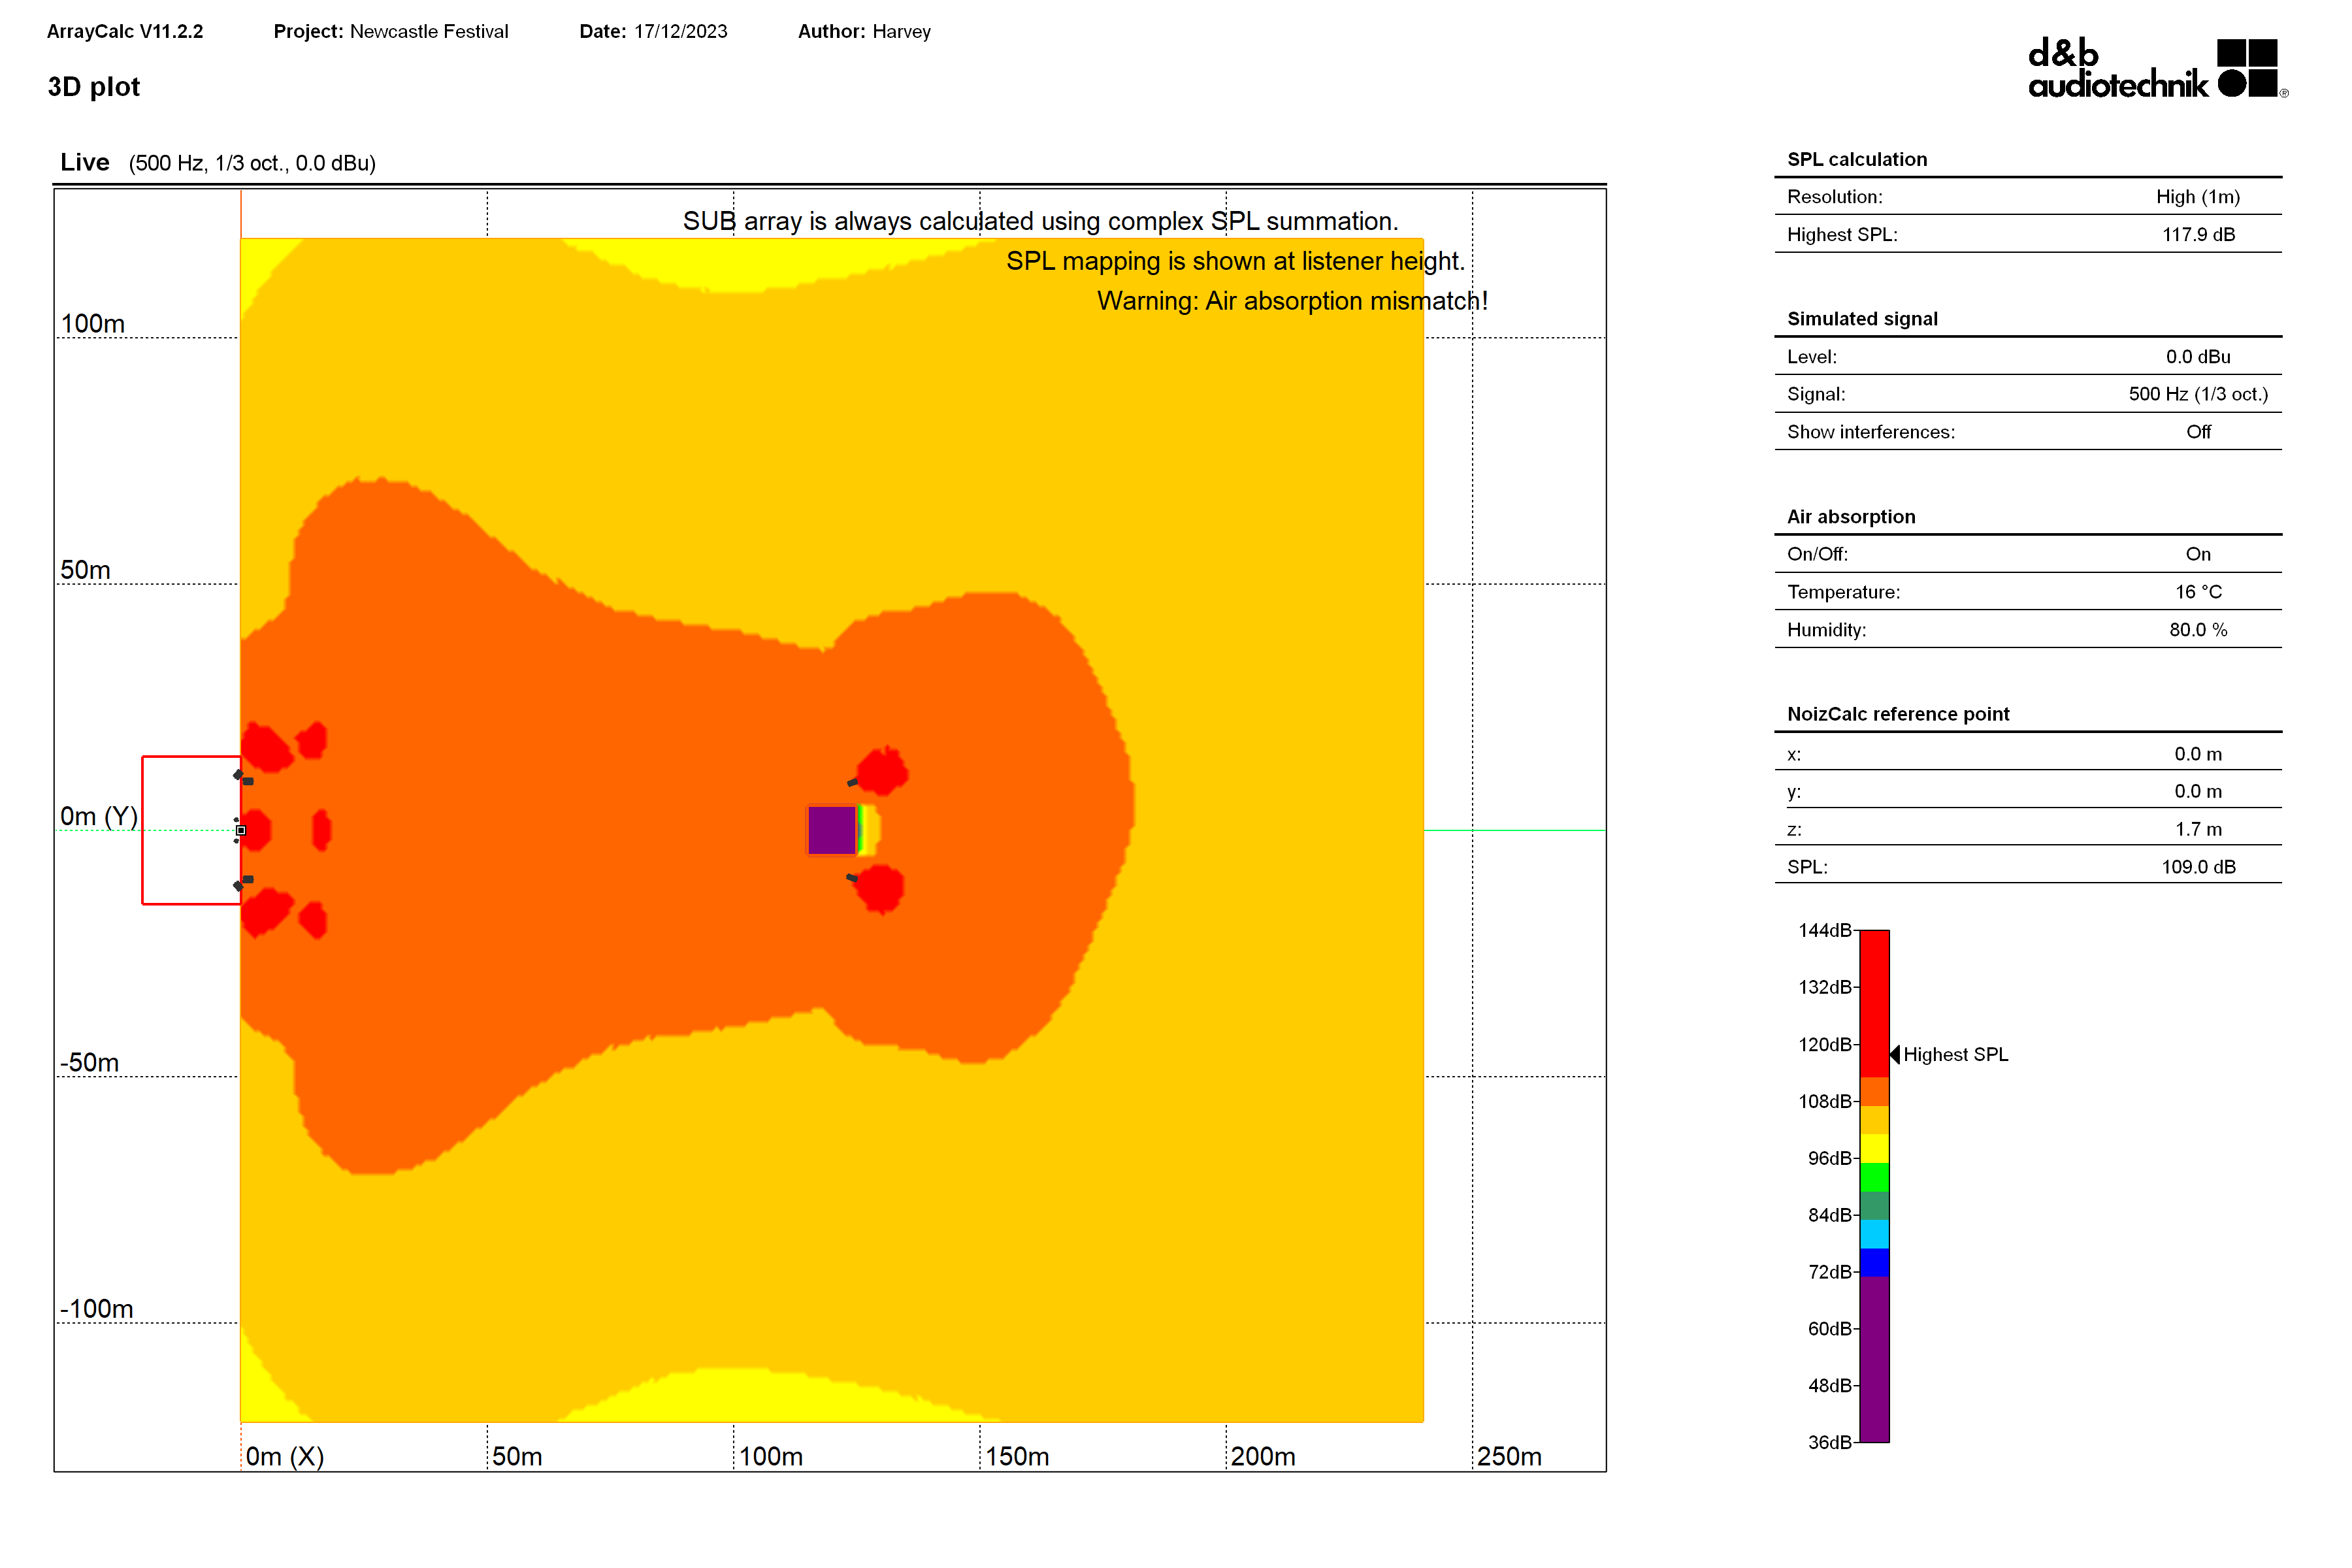
\includegraphics[width=0.5\textwidth]{Images/spl_plot_500hz.png}}      & \multicolumn{1}{c|}{\SI{117.9}{\dB}} & \multicolumn{1}{c|}{\SI{96}{\dB}}  & \multicolumn{1}{c|}{\SI{15.5}{\dB}} & \SI{107.0}{\dB} \\ \hline
            \multicolumn{1}{|c|}{\SI{1}{\kHz}}  & \multicolumn{1}{c|}{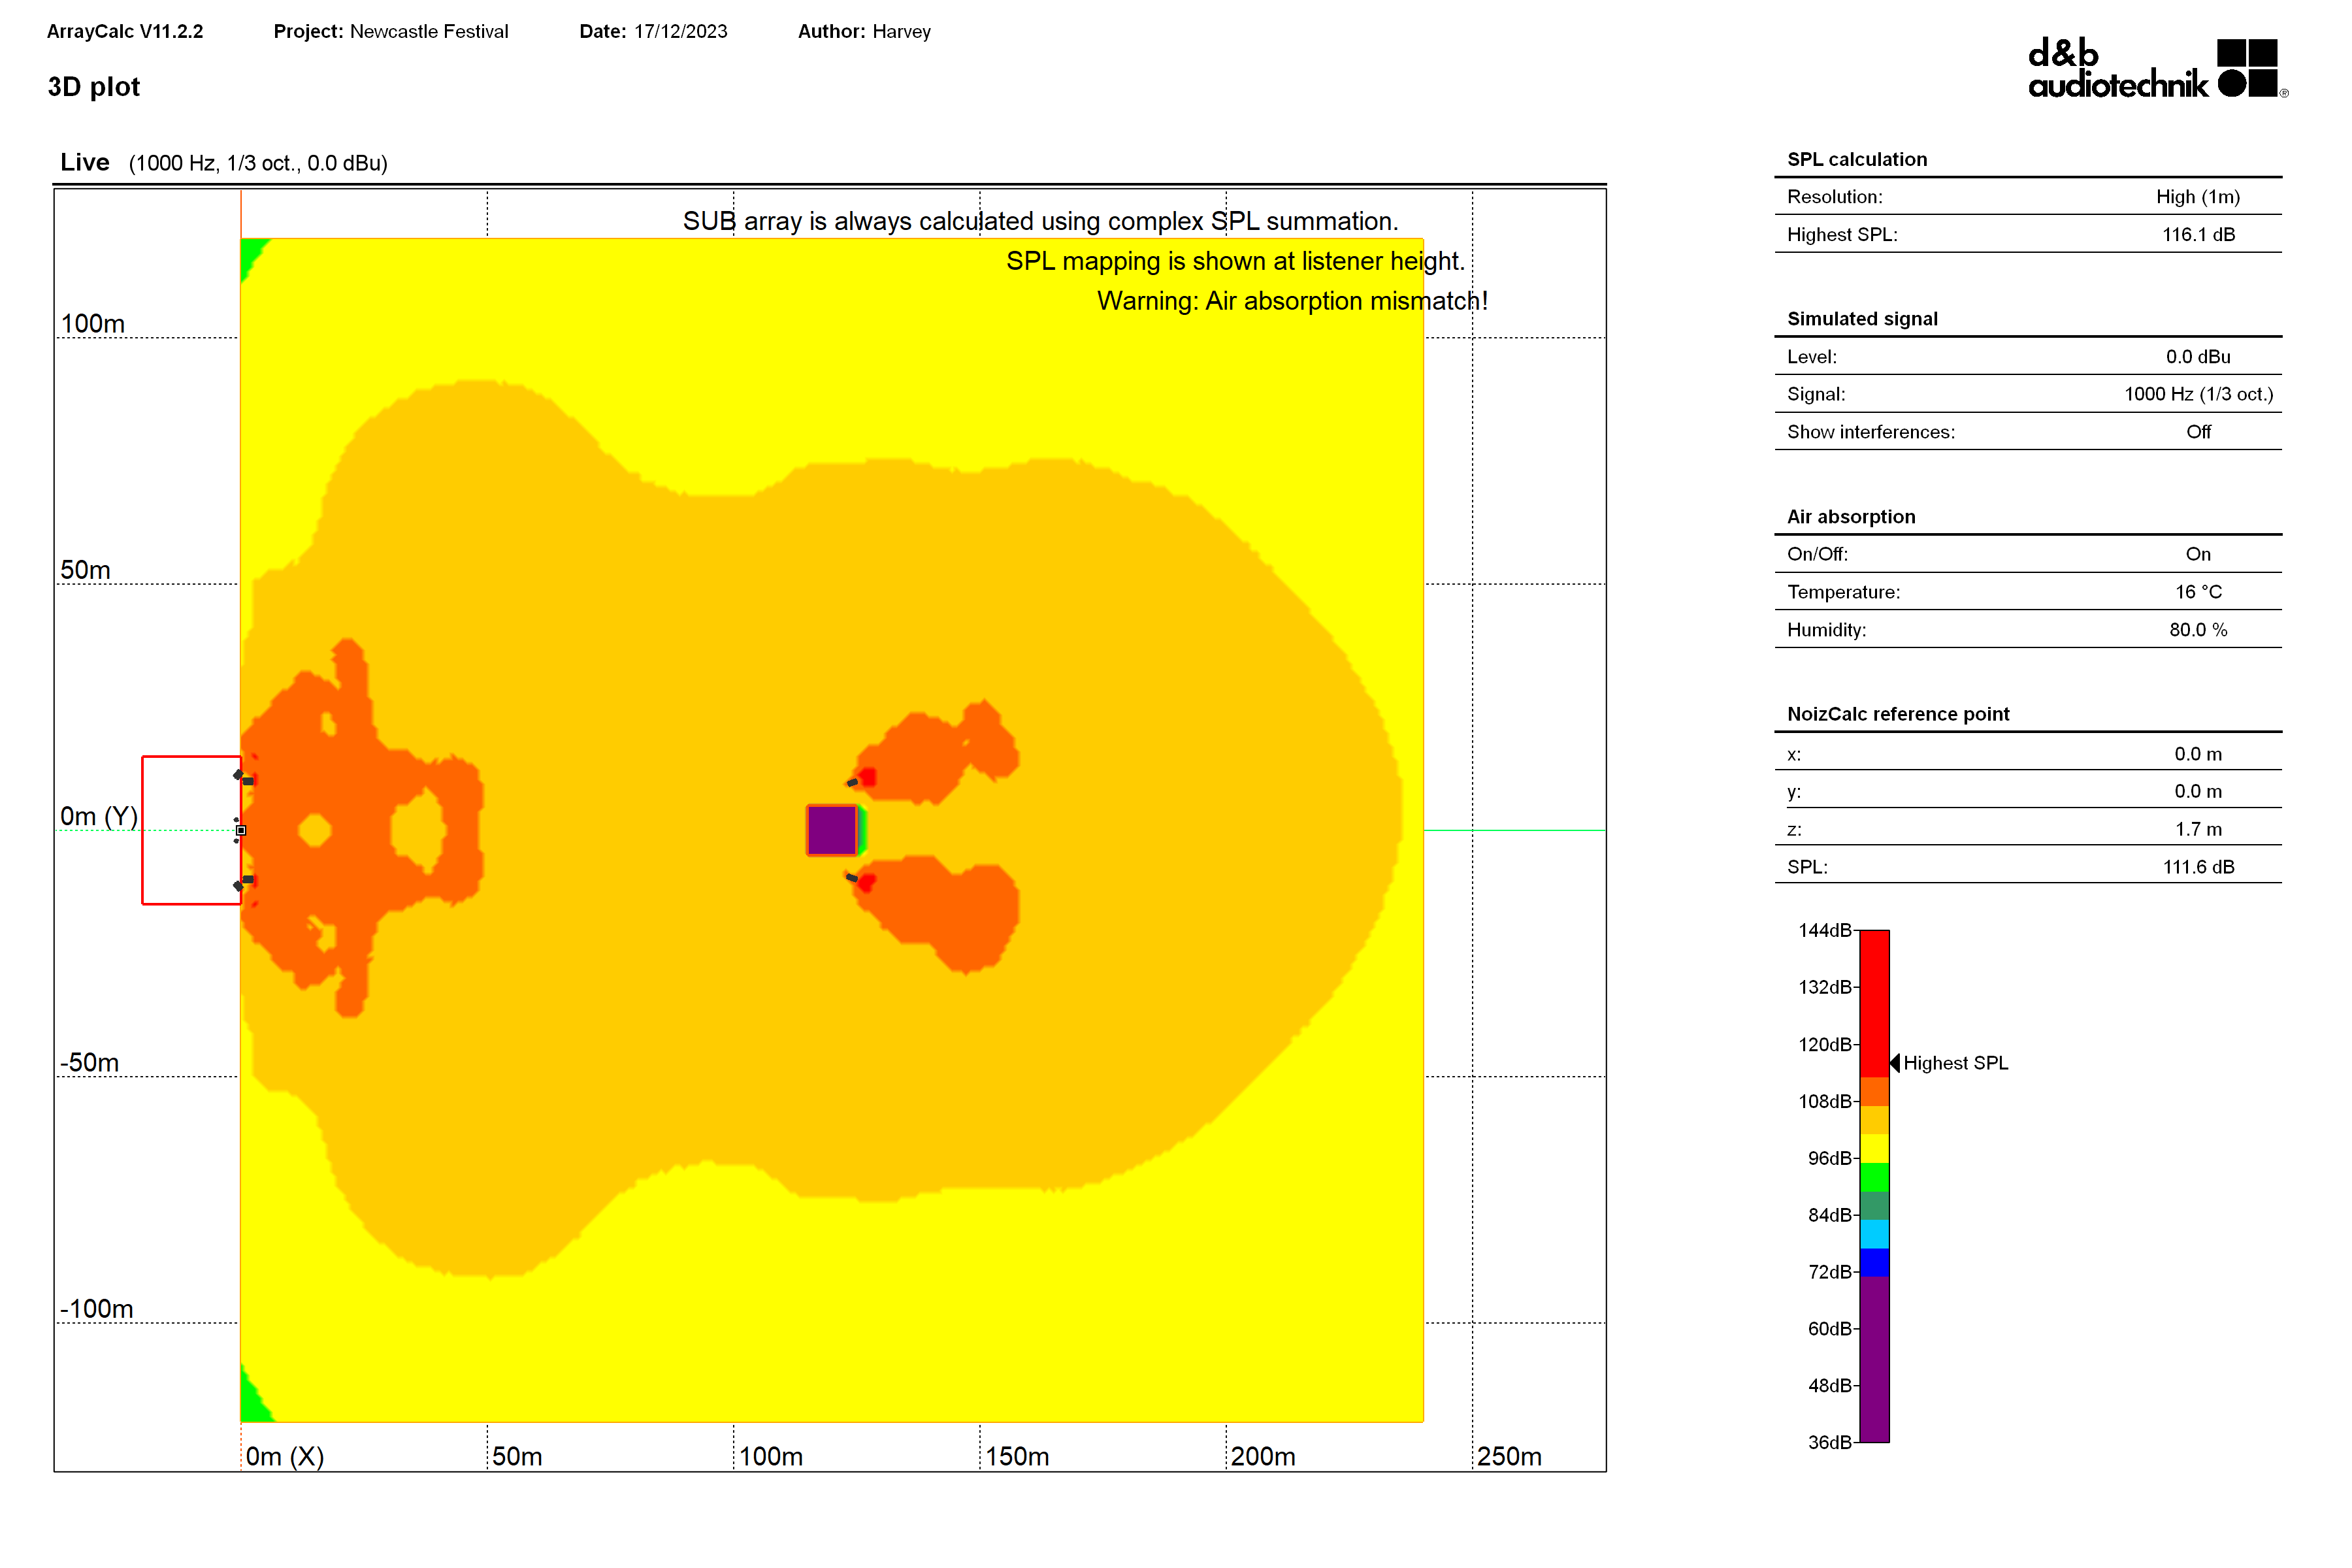
\includegraphics[width=0.5\textwidth]{Images/spl_plot_1khz.png}}       & \multicolumn{1}{c|}{\SI{116.1}{\dB}} & \multicolumn{1}{c|}{\SI{90}{\dB}}  & \multicolumn{1}{c|}{\SI{18.5}{\dB}} & \SI{103.1}{\dB} \\ \hline
            \multicolumn{1}{|c|}{\SI{2}{\kHz}}  & \multicolumn{1}{c|}{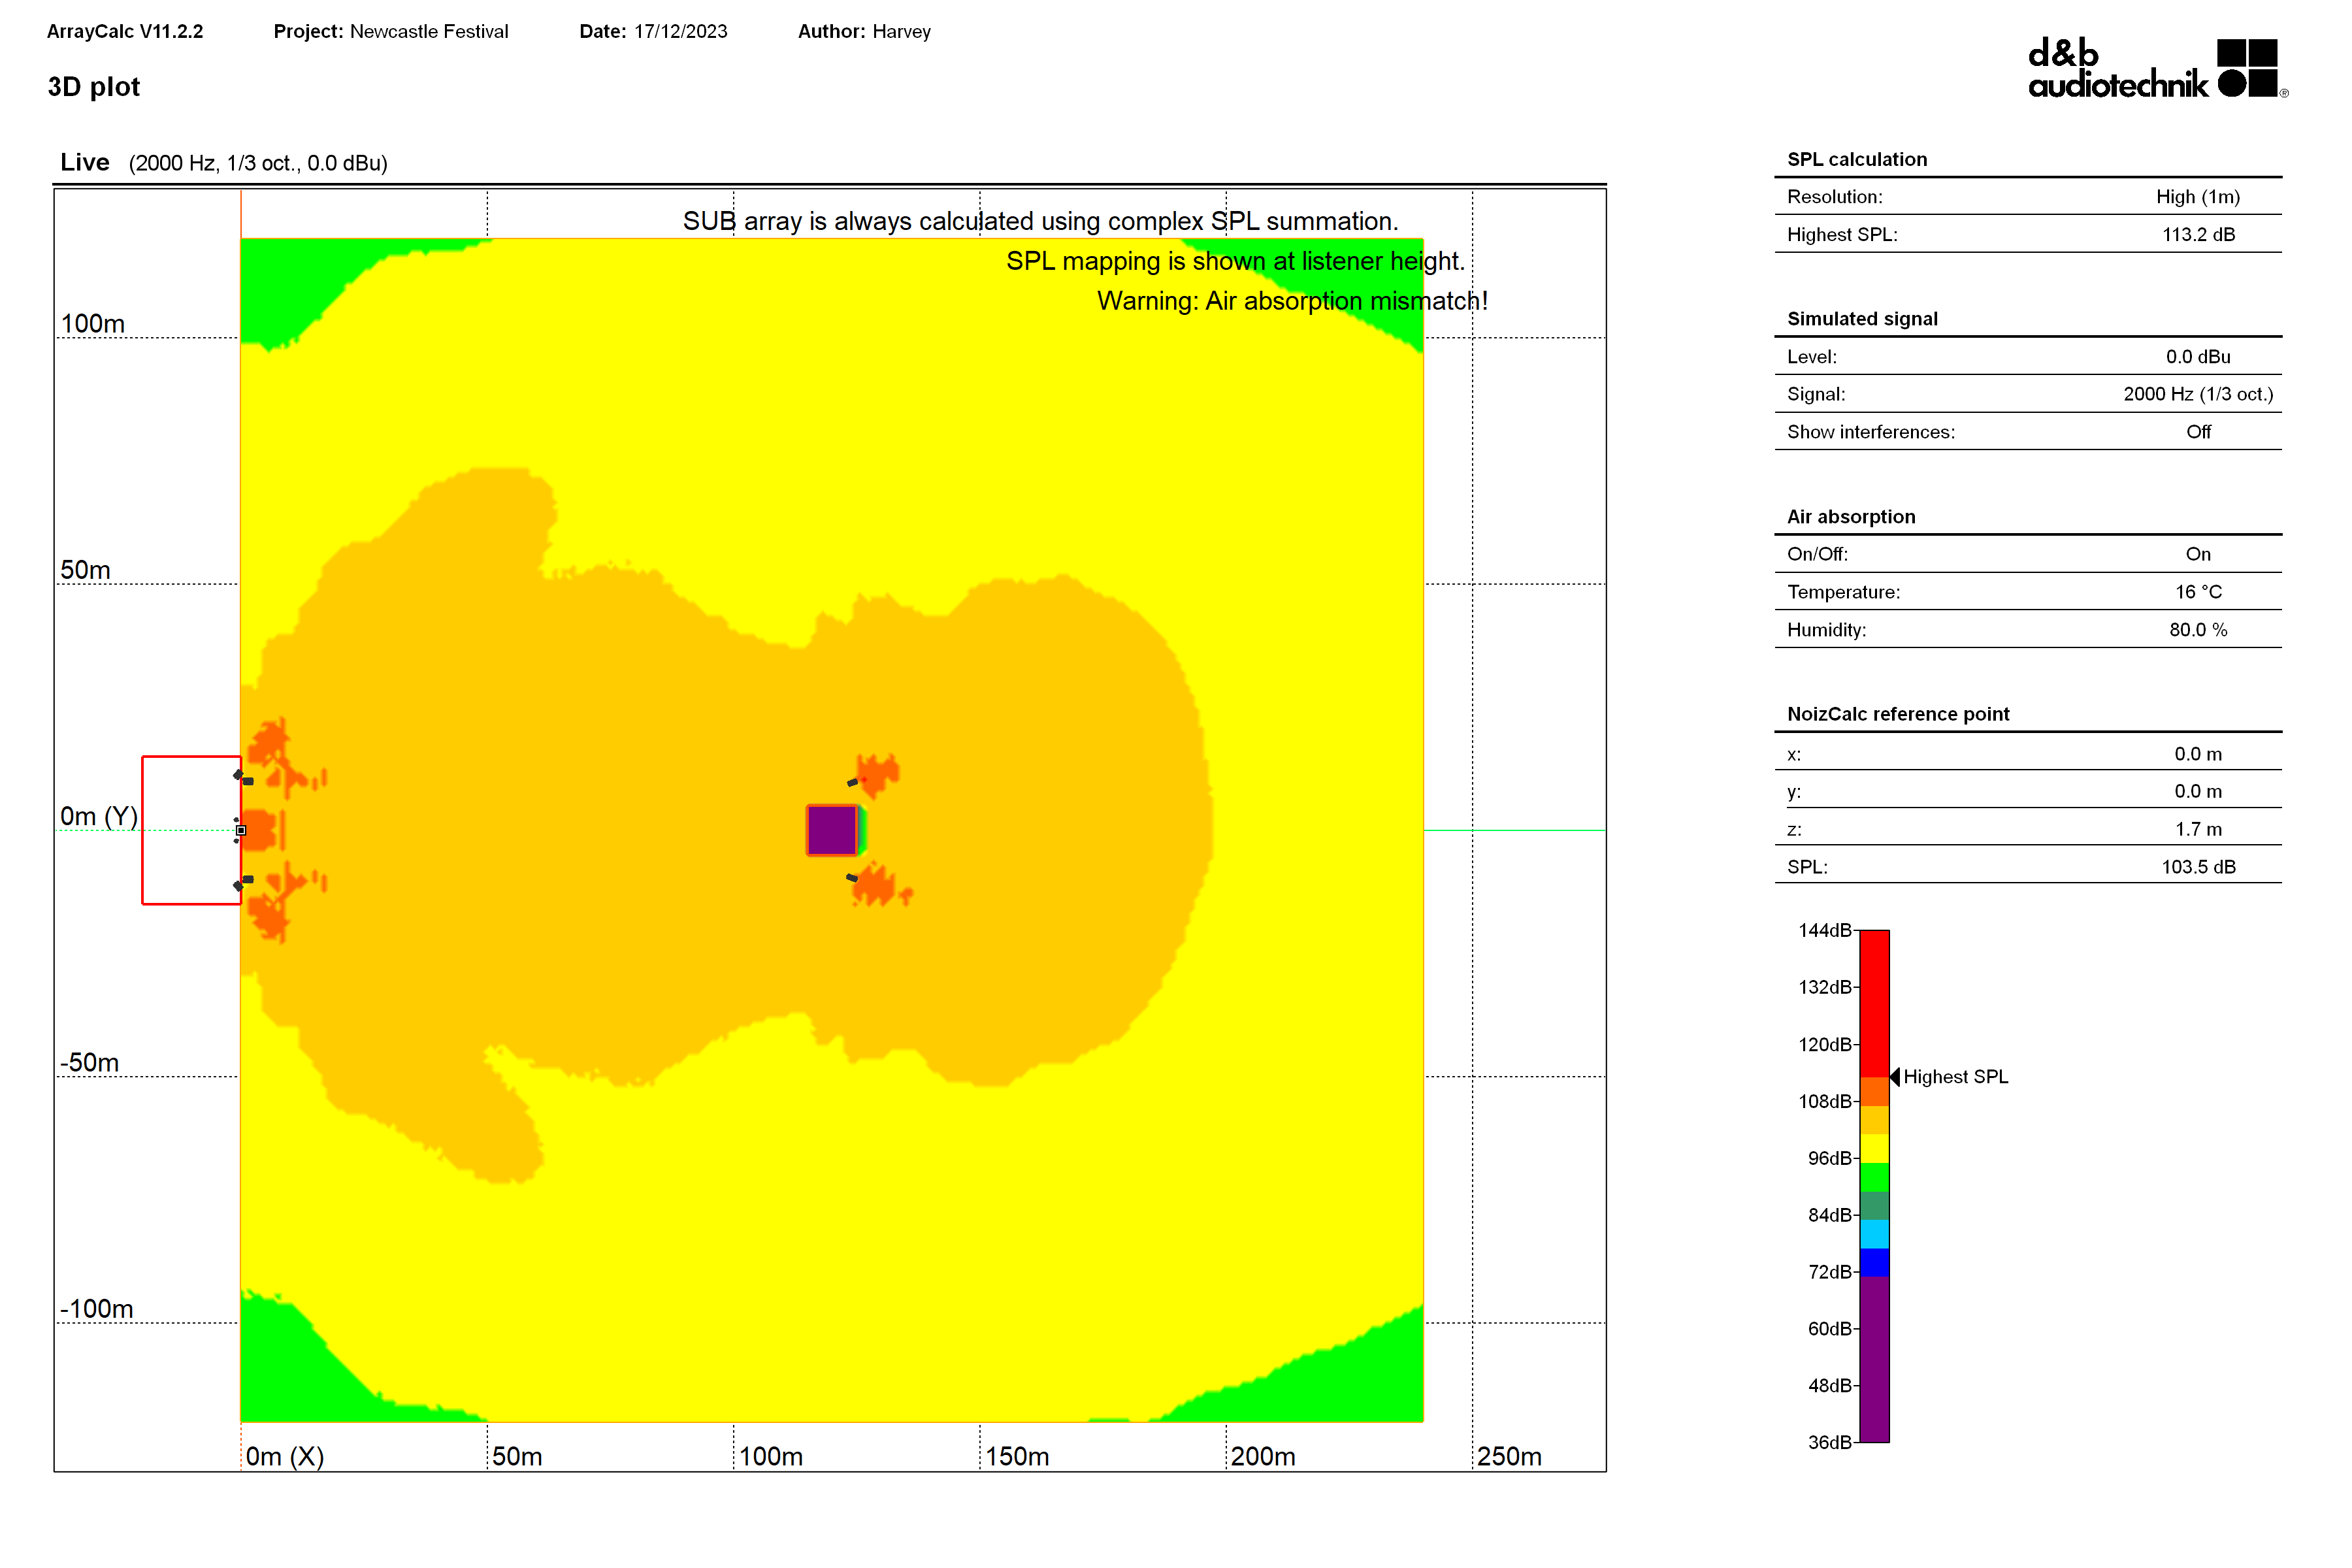
\includegraphics[width=0.5\textwidth]{Images/spl_plot_2khz.png}}       & \multicolumn{1}{c|}{\SI{116.1}{\dB}} & \multicolumn{1}{c|}{\SI{90}{\dB}}  & \multicolumn{1}{c|}{\SI{18.5}{\dB}} & \SI{103.1}{\dB} \\ \hline
            \multicolumn{1}{|c|}{\SI{5}{\kHz}}  & \multicolumn{1}{c|}{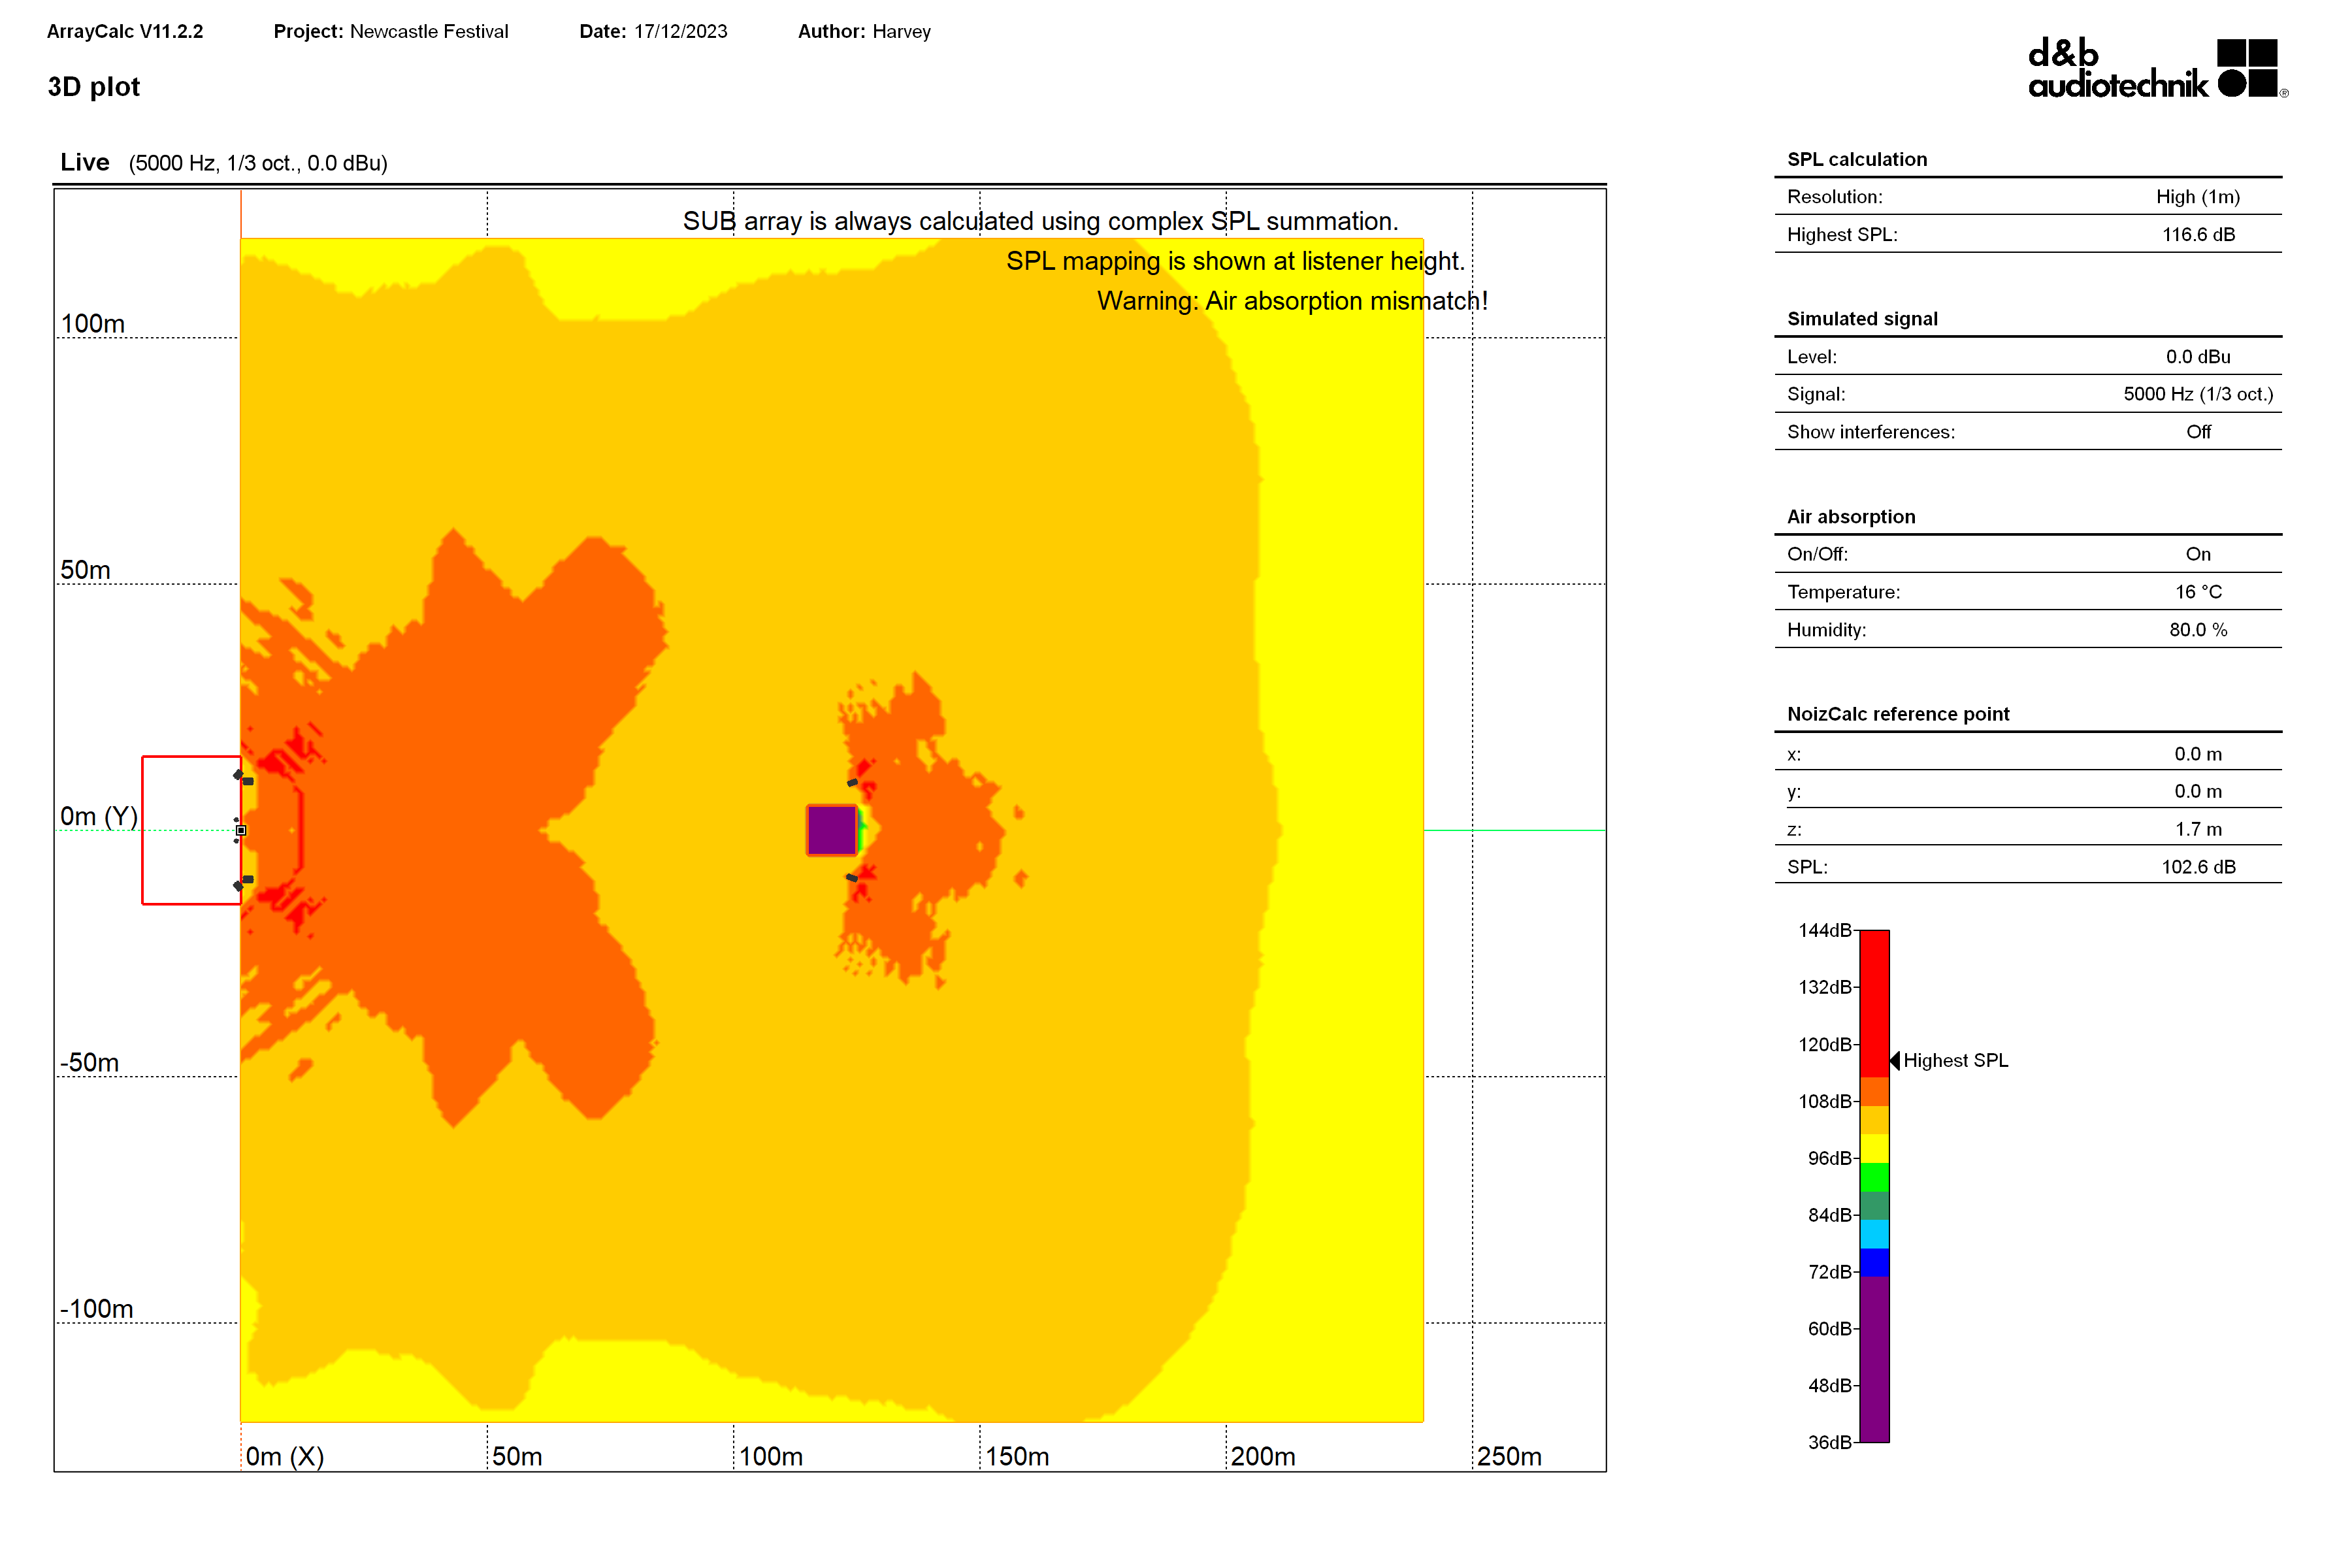
\includegraphics[width=0.5\textwidth]{Images/spl_plot_5khz.png}}       & \multicolumn{1}{c|}{\SI{116.6}{\dB}} & \multicolumn{1}{c|}{\SI{96}{\dB}}  & \multicolumn{1}{c|}{\SI{14.6}{\dB}} & \SI{106.3}{\dB} \\ \hline
            \multicolumn{1}{|c|}{\SI{10}{\kHz}} & \multicolumn{1}{c|}{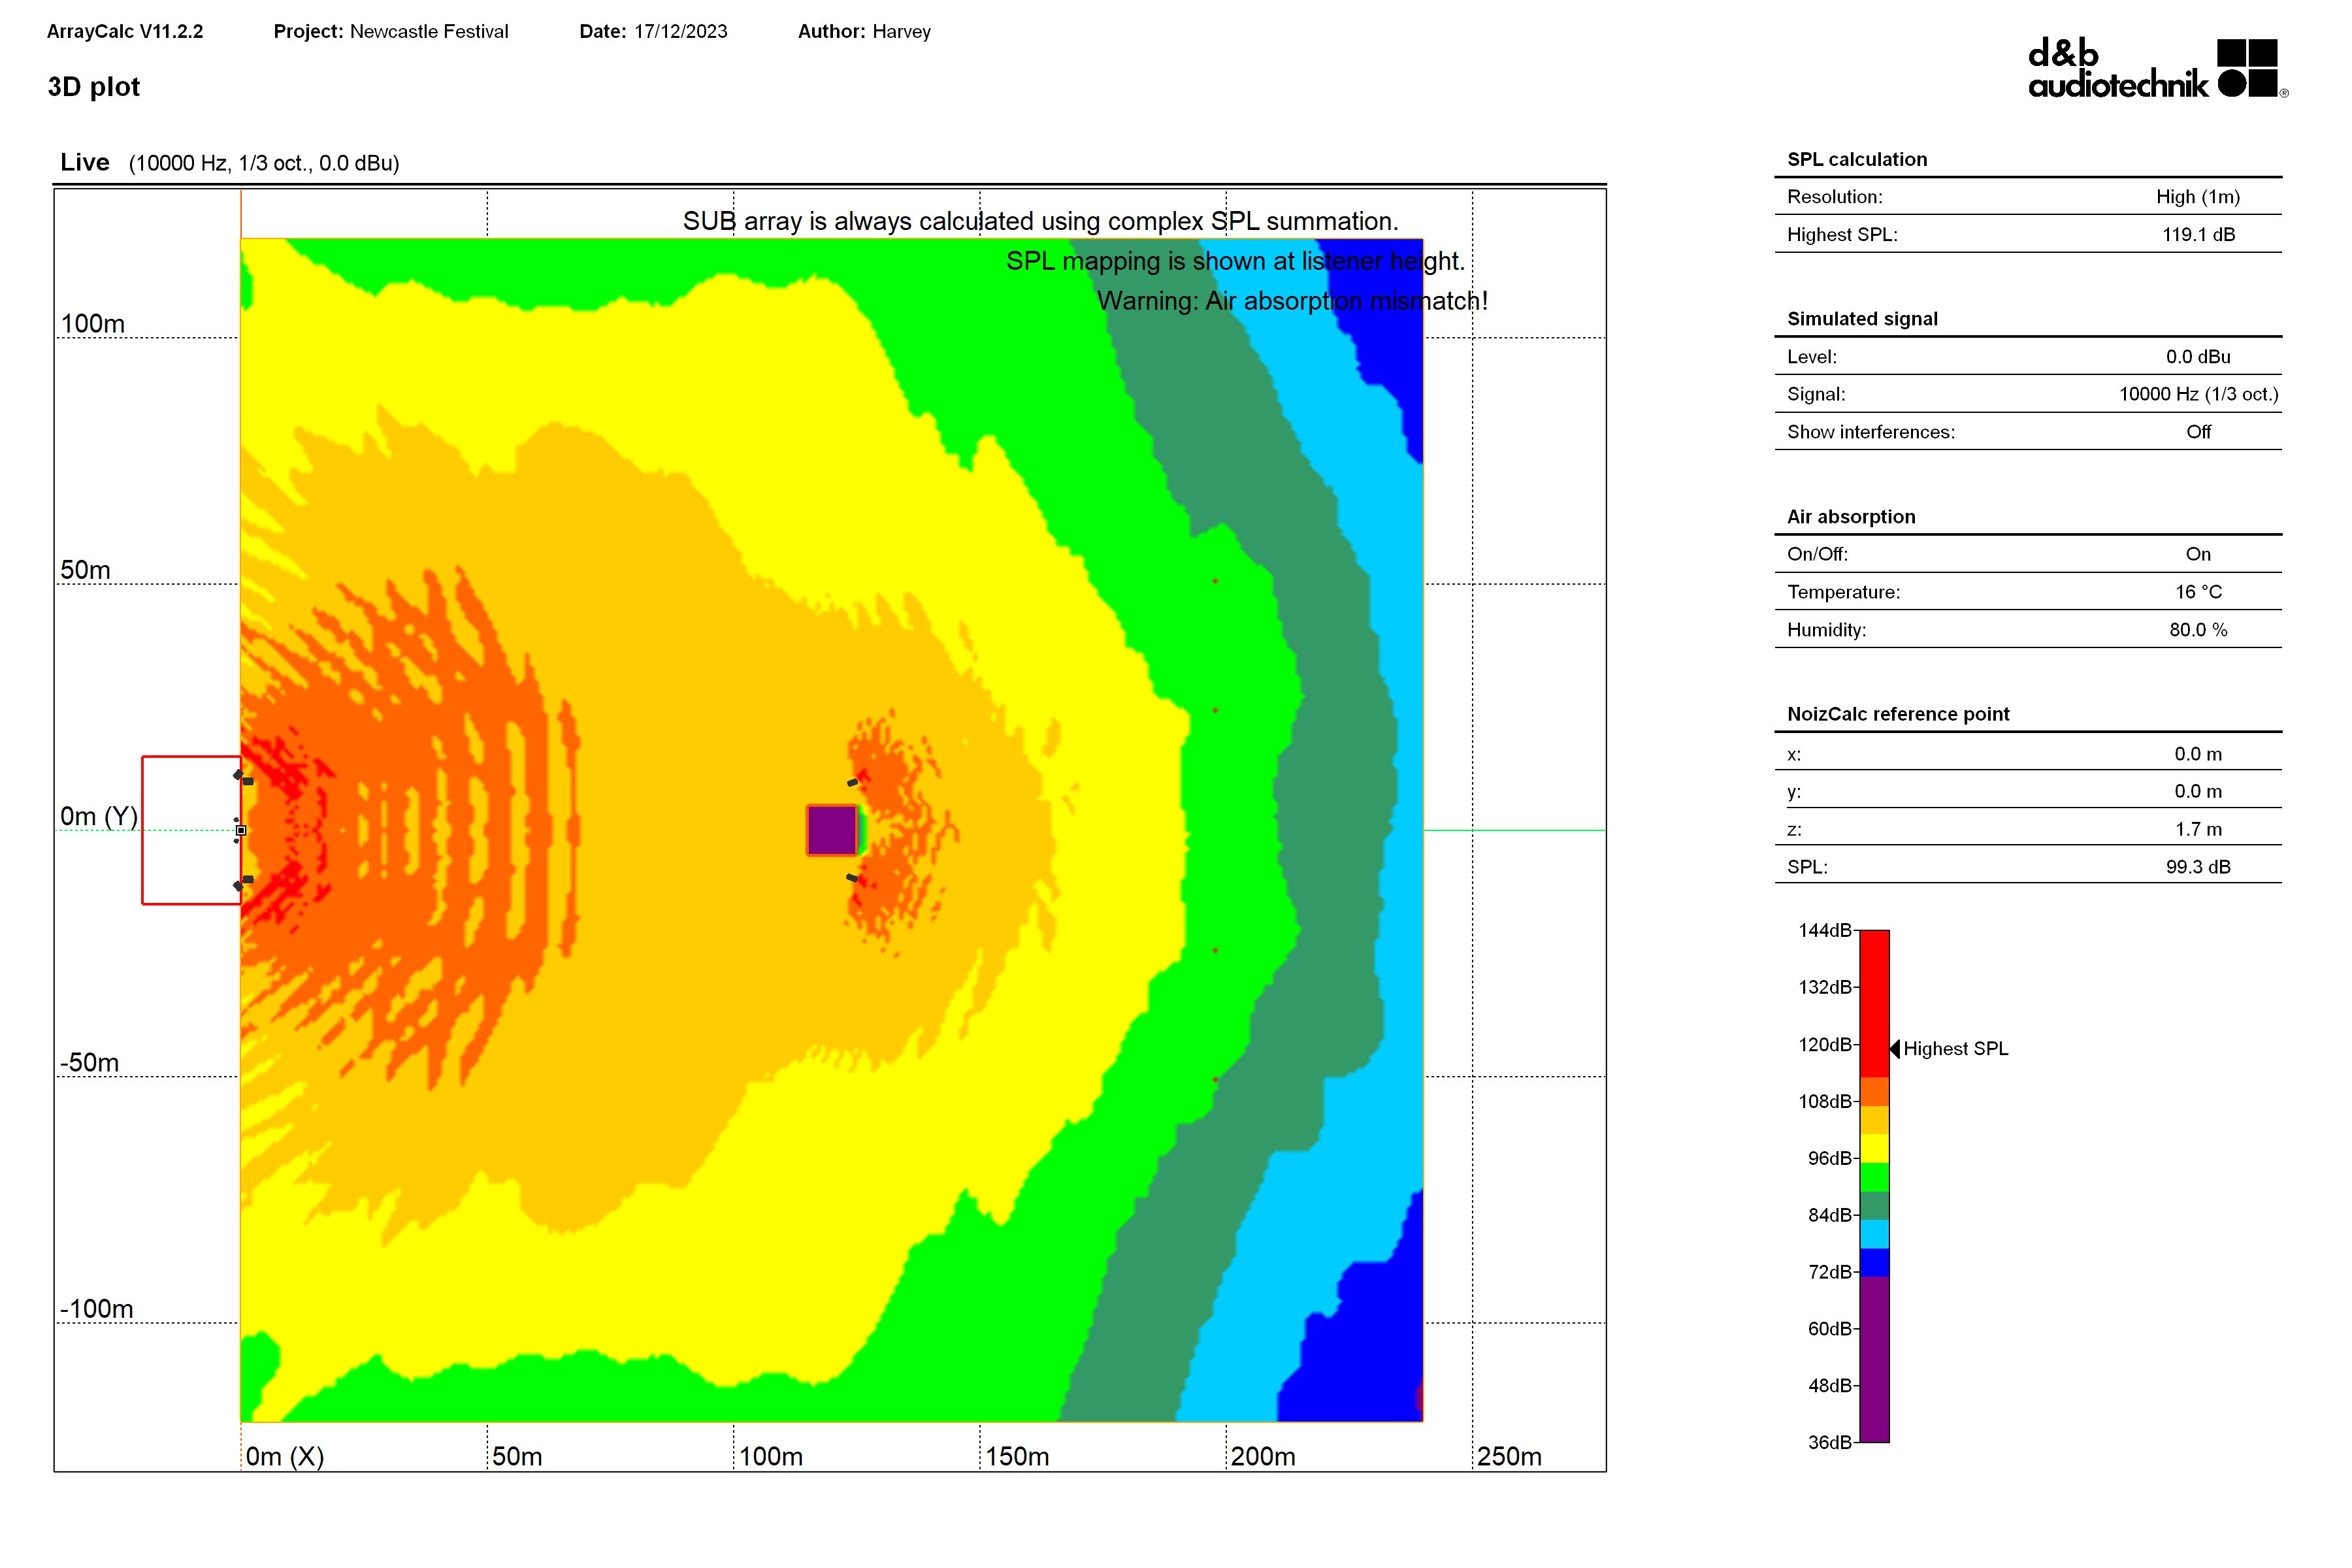
\includegraphics[width=0.5\textwidth]{Images/spl_plot_10khz.png}}      & \multicolumn{1}{c|}{\SI{119.1}{\dB}} & \multicolumn{1}{c|}{\SI{72}{\dB}}  & \multicolumn{1}{c|}{\SI{33.3}{\dB}} & \SI{95.6}{\dB} \\ \hline
            \multicolumn{1}{|c|}{Pink}          & \multicolumn{1}{c|}{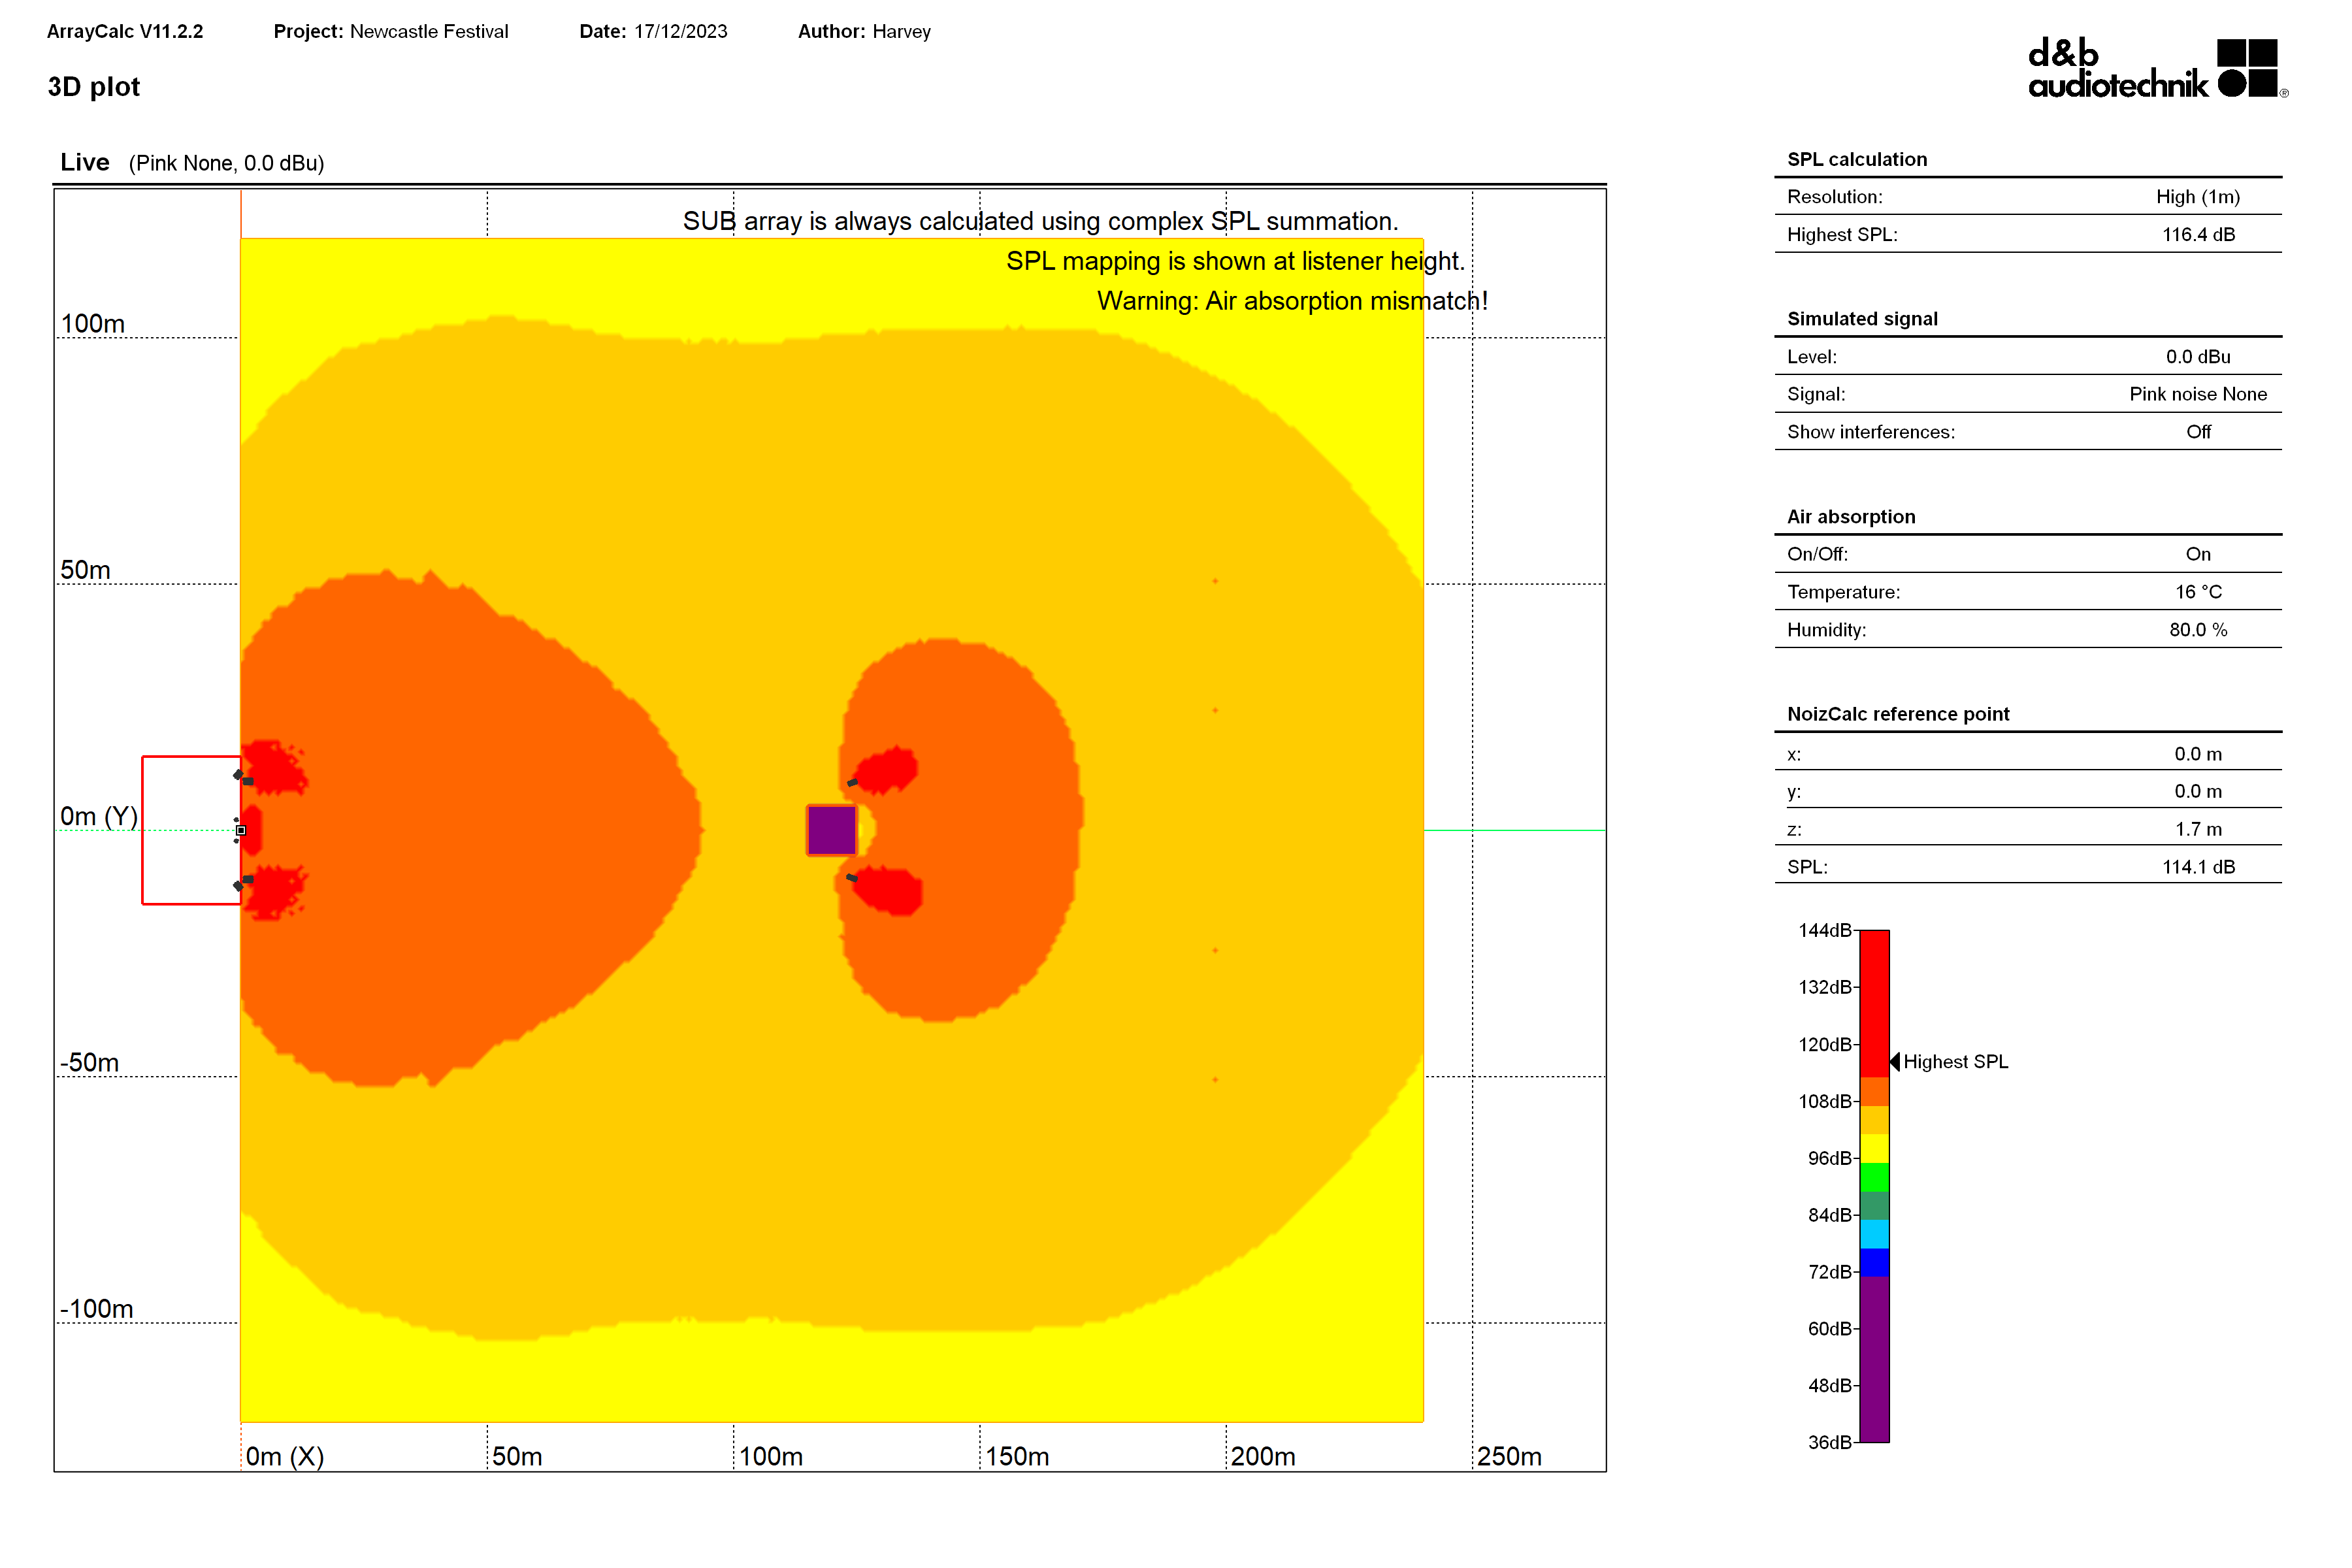
\includegraphics[width=0.5\textwidth]{Images/spl_plot_pink_none.png}}  & \multicolumn{1}{c|}{\SI{116.4}{\dB}} & \multicolumn{1}{c|}{\SI{96}{\dB}}  & \multicolumn{1}{c|}{\SI{14.4}{\dB}} & \SI{106.2}{\dB} \\ \hline
            
            \caption{SPL Mapping}
            \label{tab:spl_mapping}
        \end{longtable}

        \subsubsection{Monitors}
            As regards to monitors, the band will use \gls{iem}s, however the requested sub side fills will require an additional 2 d\&b V-GSubs and a d\&b D20 Amplifier.
            
        \subsubsection{Design Considerations}            
            NoizCalc was used to calculate the noise pollution (Figure \ref{fig:noise_pollution}). This takes into account the temperature, humidity, altitude and obstacles such as greenery or structures. Although this may not be fully accurate and is variable depending upon meteorological conditions, it gives a good approximation.

            \citet{lwestbury2016} also stated that some events offer to pay for temporary relocation of residents in the immediate locality if needed or even provide free and discounted tickets to residents within a certain radius of the event.
            
            \begin{figure}[H]
                \centering
                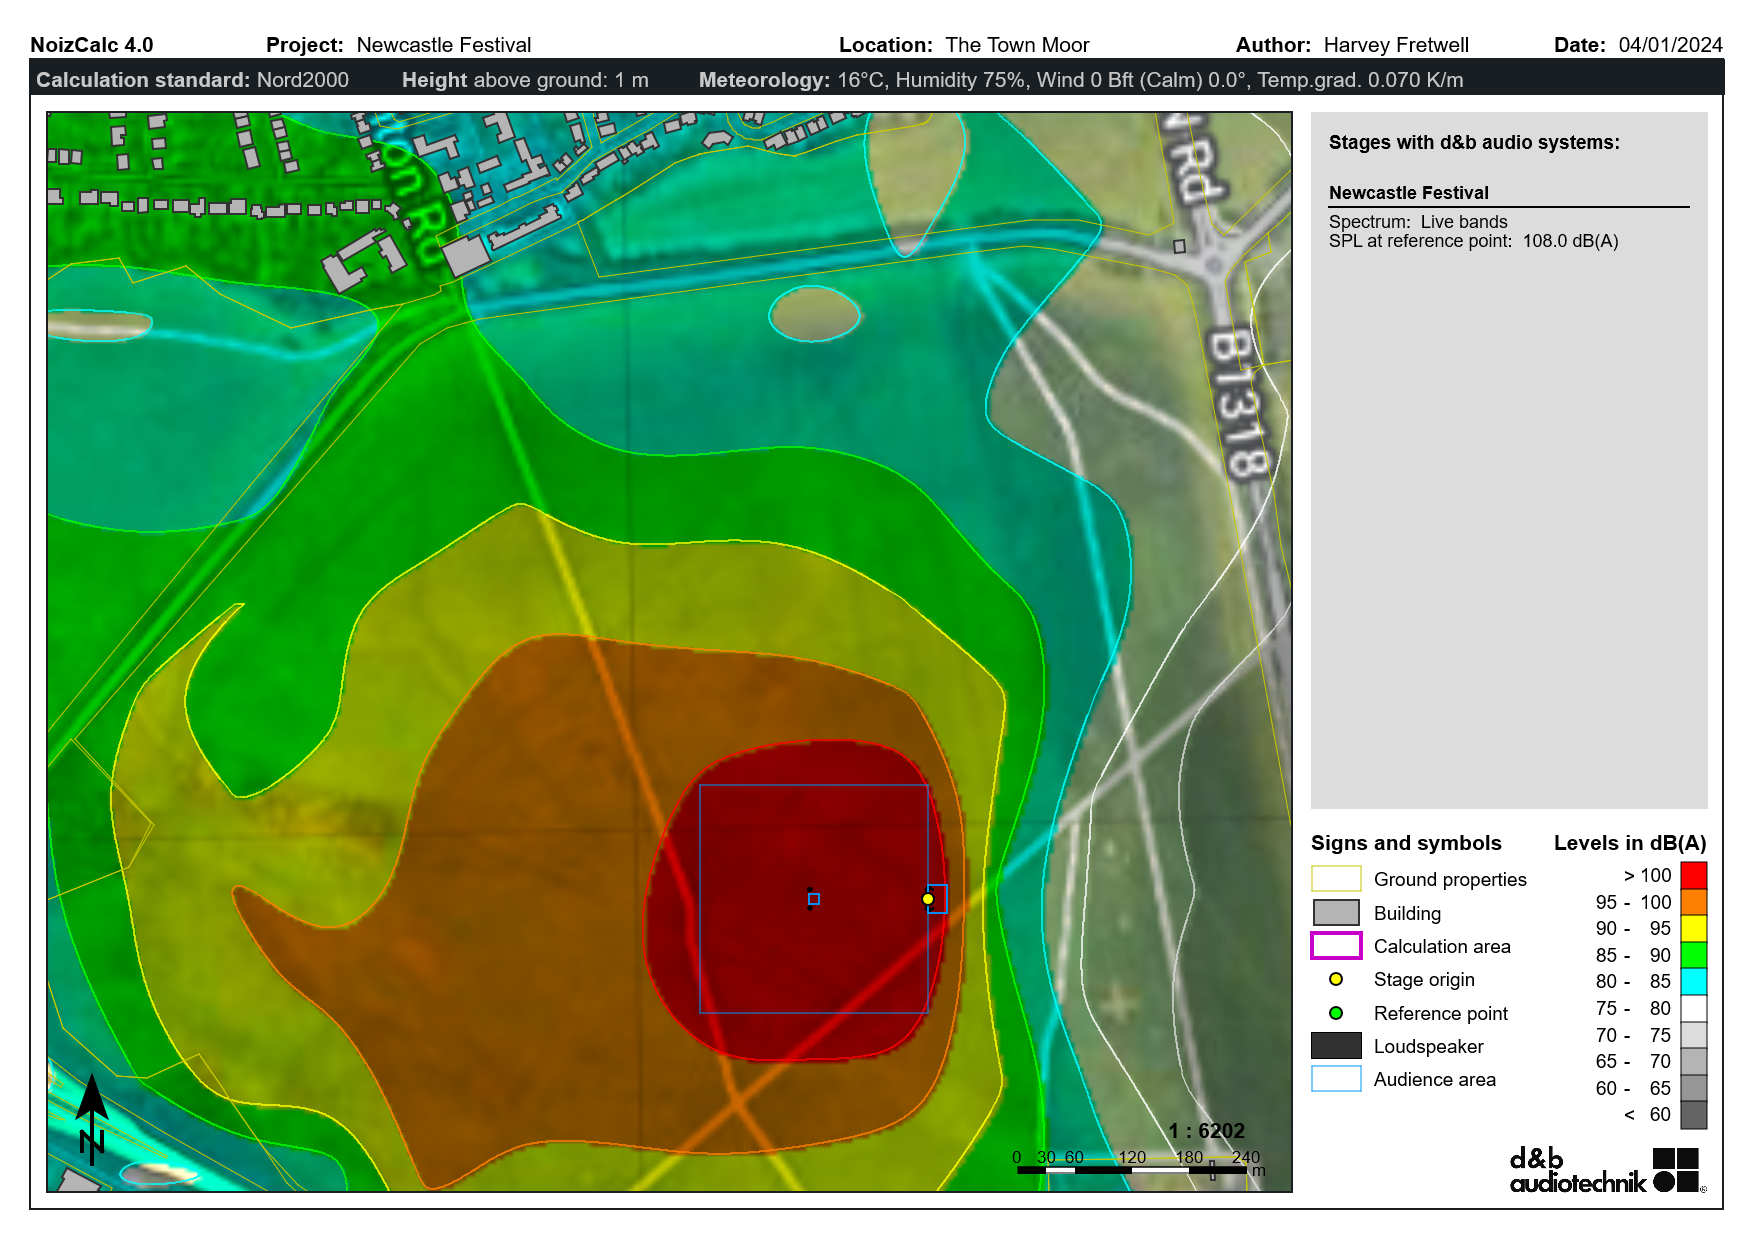
\includegraphics[width=1\linewidth]{Images/noise_polution.png}
                \caption{Noise pollution for the surrounding area}
                \label{fig:noise_pollution}
            \end{figure}

    \subsection{System Selection}        
        \subsubsection{Console}
            Various consoles were explored and after comparing the tech specs against the price ranges, the following consoles came out as the most appropriate for the festival at an affordable price range (baring in mind these prices are for buying outright, not hiring) \ref{tab:console_comparison}. Other consoles such as the Yamaha Rivage PM series and the DiGiCo Quantum series had more features but drastically increased in price.
            
            The final console chosen was the DiGiCo SD12 for both \gls{foh} and Monitors as although the band specified DiGiCo SD10's, the SD12 is more expandable when using Dante and Waves, and the usability will be analogous. Features such as the extensive \gls{dsp}, high channel count, busses/matrices provides optimal flexibility for the engineers. 2 large touchscreens with 26 touch sensitive and motorised faders will increase usability. These desks also provide high quality audio with less than \SI{0.05}{\percent} \gls{thd} and up to 40-bit floating point processing. Having the expandability of Waves on the monitors will provide even extra \gls{dsp}.

            \begin{longtable}[H]{|p{3cm}|>{\columncolor[HTML]{9AFF99}}p{3.1cm}|>{\columncolor[HTML]{FFCCC9}}p{3.1cm}|>{\columncolor[HTML]{FFDDB4}}p{3.1cm}|>{\columncolor[HTML]{FFDDB4}}p{3.1cm}|}
                \hline
                \textbf{} & \textbf{DiGiCo SD12} & \textbf{Yamaha CL3} & \textbf{Midas HD 96} & \textbf{Soundcraft Vi5000} \\ \hline
                \endfirsthead
                \endhead
                \textbf{Channels} & 64 I/O over Dante (+8 I/O on the desk) & 64 I/O over Dante (8 I/O on the desk) & 64 I/O over Dante (+8 I/O on the desk) & 64 I/O over Dante \\ \hline
                \textbf{Buses} & 36 mix, 12 Matrix & 24 mix, 8 matrix & 96 mix, 24 matrix & 32 mix, 8 matrix \\ \hline
                \textbf{Touchscreen Control} & 2x 15 inch & 10 inch & 21 inch & 4x 10 inch \\ \hline
                \textbf{Faders} & 26 Touch-Sensitive, Motorised & 26 Motorised & 28 Touch-Sensitive, Motorised & 32 Touch-Sensitive, Motorised \\ \hline
                \textbf{Sample Rate} & \SI{96}{\kHz} with Dante & \SI{48}{\kHz} & \SI{96}{\kHz} & \SI{96}{\kHz} \\ \hline
                \textbf{Effects} & 119 Dynamic EQs, 119 DigiTubes, 12 Digital Effects & 8 GEQ Racks, 8 Effect Racks, 8 Premium Racks & 24 Effects Slots, 84 Ultima Dynamic EQs & 8 Stereo Lexicon multi-effects units, UAD powered plugin platform \\ \hline
                \textbf{Existing Connectivity} & MADI & Dante & AES50 & MADI \\ \hline
                \textbf{Expansion Cards Needed} & DMI-DANTE64@96, DMI-WAVES & WSG-Y16 V3 mini-YGDAI I/O & KT-DANTE64, Soundgrid not supported & VI-DANTE, Soundgrid not supported \\ \hline
                \textbf{Price (Approx.)} & £20,500 & £20,000 & £30,000 & £30,000 \\ \hline
                \textbf{Card Price (Approx.)} & £1,586 + £931 & £549 & £677 & £1,444 \\ \hline
                \caption{Console Comparison (Green: 1\textsuperscript{st}, Orange 2\textsuperscript{nd}, Red 3\textsuperscript{rd})}
                \label{tab:console_comparison}
            \end{longtable}

        \subsubsection{Stage Box}
            Various stage boxes were compared (as shown in Table \ref{tab:stagebox_comparison}) including the Yamaha Pio series, however these were only compatible with Rivage consoles. As both consoles are DiGiCo, the SD-Rack will be used for the stage box as this allows for gain and phantom control via the desk. To make this Dante compatible, an Orange Box will be needed to convert from Dante to OPTO or an OPTO card can be added onto the SD12 console.

            \begin{longtable}[H]{|p{3cm}|>{\columncolor[HTML]{9AFF99}}p{3cm}|>{\columncolor[HTML]{FFCCC9}}p{3cm}|>{\columncolor[HTML]{FFCE93}}p{3cm}|>{\columncolor[HTML]{FFCE93}}p{3cm}|}
            \hline
                \textbf{} & \textbf{DiGiCo SD-Rack} & \textbf{Yamaha RIO3224} & \textbf{Soundcraft Vi 6432} & \textbf{Allen \& Heath dLive CDM64} \\ \hline
                \endfirsthead
                \endhead
                %
                \textbf{Channels} &
                  56 Analogue Inputs, 56 Analogue Outputs &
                  32 Analog Inputs, 16 Outputs, 8 Digital Outputs, Would require 2x &
                  64 Analogue Inputs, 32 Analogue Outputs &
                  64 Analogue Inputs, 32 Analogue Outputs \\ \hline
                \textbf{Sample Rate} &
                  \SI{96}{\kHz} &
                  \SI{96}{\kHz} &
                  \SI{96}{\kHz} &
                  \SI{96}{\kHz} \\ \hline
                \textbf{Existing Connectivity} &
                  MADI, Opto &
                  Dante &
                  MADI &
                  DX \\ \hline
                \textbf{Expansion Cards Needed} &
                  Orange Box &
                  - &
                  VI-DANTE &
                  M-DANTE A \\ \hline
                \textbf{Price (Approx.)} &
                  £10,011 &
                  £9,280 x2 &
                  £11,981 &
                  £9,272 \\ \hline
                \textbf{Card Price} &
                  £1,188 &
                  - &
                  £1,444 &
                  £990 \\ \hline
                  \caption{Stagebox Comparison (Green: 1\textsuperscript{st}, Orange 2\textsuperscript{nd}, Red 3\textsuperscript{rd})}
                \label{tab:stagebox_comparison}
            \end{longtable}
            
        \subsubsection{Monitors}
            The band has requested L'acoustics SB28JKS28 as sub sidefills however, our system is using a d\&b audiotechnik system, therefore V-GSUBs have been substituted. A buttkicker will be provided for the drummer as it is a common preference to help feel the bass when using \gls{iem}s. All other monitors will be \gls{iem}s.
            
        \subsubsection{IEM}
            Wireless microphones and \gls{iem}s, typically operate within specific radio frequency bands:

            \begin{itemize}
                \item \textbf{\gls{vhf}}: Frequencies between \SI{30}{\MHz} and \SI{300}{\MHz}. While \gls{vhf} was historically popular for wireless microphones, it has become less common due to its susceptibility to interference and limited available spectrum.
                \item \textbf{\gls{uhf}}: Frequencies between \SI{300}{\MHz} and \SI{3}{\GHz}. \gls{uhf} is widely used in the professional audio industry for wireless microphones and \gls{iem}. It offers a larger available spectrum, which allows for more channels and better resistance to interference compared to \gls{vhf}.
            \end{itemize}

            \citep{shure2024}

            Table \ref{tab:frequency_range_licensing} shows the frequency bands and their required licensing.

            \begin{longtable}[H]{|p{2.5cm}p{11cm}|}
                \hline
                \multicolumn{1}{|l|}{\textbf{Frequency Ranges}} &
                  \textbf{Licensing Information} \\ \hline
                \endfirsthead
                %
                \endhead
                %
                \rowcolor[HTML]{FFDDB4} 
                \multicolumn{1}{|l|}{\cellcolor[HTML]{FFDDB4}\SI{470}{} – \SI{550}{\MHz}} &
                  Mandates licensing and is exclusively sanctioned for use in installations, major events, and specialised applications. \\ \hline
                \rowcolor[HTML]{FFFC9E} 
                \multicolumn{1}{|l|}{\cellcolor[HTML]{FFFC9E}\SI{550}{} – \SI{558}{\MHz}} &
                  Needs a license that lasts for 6 months (renewable), commonly set aside for LTE, and is contingent upon individual local authorisation verifications. \\ \hline
                \rowcolor[HTML]{FFFC9E} 
                \multicolumn{1}{|l|}{\cellcolor[HTML]{FFFC9E}\SI{566}{} – \SI{606}{\MHz}} &
                  \cellcolor[HTML]{FFFC9E}Needs a license that lasts for 6 months (renewable), commonly set aside for LTE, and is contingent upon individual local authorisation verifications. \\ \hline
                \rowcolor[HTML]{FFDDB4} 
                \multicolumn{1}{|l|}{\cellcolor[HTML]{FFDDB4}\SI{606}{} – \SI{614}{\MHz}} &
                  Primary band, necessitates an annual license fee of £85. \\ \hline
                \rowcolor[HTML]{FFDDB4} 
                \multicolumn{1}{|l|}{\cellcolor[HTML]{FFDDB4}\SI{614}{} – \SI{630}{\MHz}} &
                  Secondary band, necessitates an annual license fee of £85. \\ \hline
                \rowcolor[HTML]{FFDDB4} 
                \multicolumn{1}{|l|}{\cellcolor[HTML]{FFDDB4}\SI{630}{} – \SI{670}{\MHz}} &
                  \cellcolor[HTML]{FFDDB4}Mandates licensing and is exclusively sanctioned for use in installations, major events, and specialised applications. \\ \hline
                \rowcolor[HTML]{FFDDB4} 
                \multicolumn{1}{|l|}{\cellcolor[HTML]{FFDDB4}\SI{734}{} – \SI{782}{\MHz}} &
                  \cellcolor[HTML]{FFDDB4}Mandates licensing and is exclusively sanctioned for use in installations, major events, and specialised applications. \\ \hline
                \rowcolor[HTML]{FFDDB4} 
                \multicolumn{1}{|l|}{\cellcolor[HTML]{FFDDB4}\SI{823}{} – \SI{832}{\MHz}} &
                  Mandatory licensing, requiring registration and associated with fees since 2015. \\ \hline
                \rowcolor[HTML]{FFCCC9} 
                \multicolumn{1}{|l|}{\cellcolor[HTML]{FFCCC9}\SI{838}{} – \SI{862}{\MHz}} &
                  Unauthorized for wireless system usage. \\ \hline
                \rowcolor[HTML]{9AFF99} 
                \multicolumn{1}{|l|}{\cellcolor[HTML]{9AFF99}\SI{863}{} – \SI{865}{\MHz}} &
                  No licensing is necessary throughout Europe; however, the maximum transmitted power is restricted to 10 mW. \\ \hline
                 &
                   \\ \hline
                \rowcolor[HTML]{9AFF99} 
                \multicolumn{1}{|l|}{\cellcolor[HTML]{9AFF99}\textbf{Free Band}} &
                  Unlicensed \\ \hline
                \rowcolor[HTML]{FFDDB4} 
                \multicolumn{1}{|l|}{\cellcolor[HTML]{FFDDB4}\textbf{Requires License}} &
                  Legal requirement for operation \\ \hline
                \rowcolor[HTML]{FFFC9E} 
                \multicolumn{1}{|l|}{\cellcolor[HTML]{FFFC9E}\textbf{Requires Temporary License}} &
                  Legal requirement for a limited duration \\ \hline
                \rowcolor[HTML]{FFCCC9} 
                \multicolumn{1}{|l|}{\cellcolor[HTML]{FFCCC9}\textbf{Illegal}} &
                  Operation without proper authorisation is prohibited \\ \hline

                \caption{Frequency range licensing}
                \label{tab:frequency_range_licensing}
            \end{longtable}
            
            These are then put into standard frequency band classes (Table \ref{tab:frequency_range_licensing}).
            
            \begin{longtable}[H]{|l|l|}
                \hline
                \textbf{Bands} & \textbf{Frequency   Ranges} \\ \hline
                \endfirsthead
                %
                \endhead
                %
                A1             & \SI{470}{} – \SI{516}{\MHz}               \\ \hline
                A              & \SI{516}{} – \SI{558}{\MHz}               \\ \hline
                G              & \SI{566}{} – \SI{608}{\MHz}               \\ \hline
                GB             & \SI{606}{} – \SI{648}{\MHz}               \\ \hline
                B              & \SI{626}{} – \SI{668}{\MHz}               \\ \hline
                C              & \SI{734}{} – \SI{776}{\MHz}               \\ \hline
                E              & \SI{823}{} – \SI{865}{\MHz}               \\ \hline
                \caption{Standard Frequency bands}
                \label{tab:frequency_band_licensing}
            \end{longtable}

            After reviewing specifications and various online reviews, the top professional \gls{iem} transmitters were Shure P10T/PSM1000 and Sennheiser SR2050.
            
            The SR2050 was chosen as it provides wide tuning bandwidths, touring-grade features, and wireless remote control via the WSM software (Table \ref{tab:iem_comparisons}). Table \ref{tab:iem_transmitter_freq_ranges} shows the various models and which frequency ranges they span. To provide minimal interference, the transmitters will span over a minimum of 2 bands i.e. Bw providing 10 channels with 72 different frequencies, spanning over GB and B bands.
            
            The Sennheiser A5000 antenna will be used on either side of the stage, as the circular polarisation minimises variations in signal strength and almost eliminates multi-path problems \citep{sennheiser-a5000}.

            \begin{longtable}[H]{|p{2cm}|
                >{\columncolor[HTML]{FFCCC9}}l |
                >{\columncolor[HTML]{FFCE93}}l |
                >{\columncolor[HTML]{FFCCC9}}l |
                >{\columncolor[HTML]{9AFF99}}l |}
                \hline
                \textbf{Feature}         & \textbf{Shure PSM900} & \textbf{Shure PSM1000} & \textbf{Sennheiser EW G4} & \textbf{Sennheiser SR2050} \\ \hline
                \endfirsthead
                %
                \endhead
                %
                Frequency Range           & 470 - 952 MHz & 470 - 952 MHz & 470 - 865 MHz & 470 - 865 MHz \\ \hline
                Compatible Frequencies    & 20 per band   & 39 per band   & 20 per band   & 20 per band   \\ \hline
                Tuning Bandwidth          & 39 - 40 MHz   & 72 - 80 MHz   & 42 MHz        & 75 MHz        \\ \hline
                Audio Frequency Response & 38 Hz - 15 kHz        & 35 Hz - 15 kHz         & 25 Hz - 15 kHz            & 25 Hz - 15 kHz             \\ \hline
                THD                       & $<\SI{0.5}{\percent}$        & $<\SI{0.5}{\percent}$        & $<\SI{0.9}{\percent}$        & $<\SI{0.9}{\percent}$        \\ \hline
                SNR                       & $>\SI{90}{\dB}$        & $>\SI{90}{\dB}$        & $>\SI{90}{\dB}$        & $>\SI{90}{\dB}$        \\ \hline
                Networking / Remote Control & No            & Yes           & No            & Yes           \\ \hline
                Rack Mountable            & No            & Yes           & Yes           & Yes           \\ \hline
                Price                     & £1,169        & £4,674        & £1,199        & £3,499        \\ \hline
                \caption{IEM Comparisons}
                \label{tab:iem_comparisons}
            \end{longtable}
            
            \begin{longtable}[H]{|p{1cm}|p{1cm}|p{1cm}|cc|cc|}
                \hline
                \textbf{Chan} &
                  \textbf{From MHz} &
                  \textbf{To MHz} &
                  \multicolumn{1}{r}{\textbf{Sennheiser}} &
                  \multicolumn{1}{l|}{\textbf{SR2050}} &
                  \multicolumn{1}{r}{\textbf{Shure}} &
                  \multicolumn{1}{l|}{\textbf{P10T}} \\ \hline
                \endfirsthead
                %
                \endhead
                %
                70 &
                  862 &
                  870 &
                  \multicolumn{1}{c|}{\cellcolor[HTML]{34FF34}DW} &
                   &
                   &
                   \\ \cline{1-3}
                \cellcolor[HTML]{FFCCC9}69 &
                  \cellcolor[HTML]{FFCCC9}854 &
                  \cellcolor[HTML]{FFCCC9}862 &
                  \multicolumn{1}{c|}{\cellcolor[HTML]{34FF34}790 - 865 MHz} &
                   &
                   &
                   \\ \cline{1-3}
                \cellcolor[HTML]{FFCCC9}68 &
                  \cellcolor[HTML]{FFCCC9}846 &
                  \cellcolor[HTML]{FFCCC9}854 &
                  \multicolumn{1}{c|}{\cellcolor[HTML]{34FF34}75 MHz} &
                   &
                   &
                   \\ \cline{1-3}
                \cellcolor[HTML]{FFCCC9}67 &
                  \cellcolor[HTML]{FFCCC9}838 &
                  \cellcolor[HTML]{FFCCC9}846 &
                  \multicolumn{1}{c|}{\cellcolor[HTML]{34FF34}} &
                   &
                   &
                   \\ \cline{1-3}
                \cellcolor[HTML]{FFCCC9}66 &
                  \cellcolor[HTML]{FFCCC9}830 &
                  \cellcolor[HTML]{FFCCC9}838 &
                  \multicolumn{1}{c|}{\cellcolor[HTML]{34FF34}} &
                   &
                   &
                   \\ \cline{1-3}
                \cellcolor[HTML]{FFCCC9}65 &
                  \cellcolor[HTML]{FFCCC9}822 &
                  \cellcolor[HTML]{FFCCC9}830 &
                  \multicolumn{1}{c|}{\cellcolor[HTML]{34FF34}} &
                   &
                   &
                   \\ \cline{1-3}
                \cellcolor[HTML]{FFCCC9}64 &
                  \cellcolor[HTML]{FFCCC9}814 &
                  \cellcolor[HTML]{FFCCC9}822 &
                  \multicolumn{1}{c|}{\cellcolor[HTML]{34FF34}} &
                   &
                   &
                   \\ \cline{1-3}
                \cellcolor[HTML]{FFCCC9}63 &
                  \cellcolor[HTML]{FFCCC9}806 &
                  \cellcolor[HTML]{FFCCC9}814 &
                  \multicolumn{1}{c|}{\cellcolor[HTML]{34FF34}} &
                   &
                   &
                   \\ \cline{1-3}
                \cellcolor[HTML]{FFCCC9}62 &
                  \cellcolor[HTML]{FFCCC9}798 &
                  \cellcolor[HTML]{FFCCC9}806 &
                  \multicolumn{1}{c|}{\cellcolor[HTML]{34FF34}} &
                   &
                   &
                   \\ \cline{1-3}
                \cellcolor[HTML]{FFCCC9}61 &
                  \cellcolor[HTML]{FFCCC9}790 &
                  \cellcolor[HTML]{FFCCC9}798 &
                  \multicolumn{1}{c|}{\cellcolor[HTML]{34FF34}} &
                   &
                   &
                   \\ \cline{1-4}
                \cellcolor[HTML]{9AFF99}60 &
                  \cellcolor[HTML]{9AFF99}782 &
                  \cellcolor[HTML]{9AFF99}790 &
                  \multicolumn{1}{c|}{\cellcolor[HTML]{38FFF8}Cw} &
                   &
                   &
                   \\ \cline{1-3}
                \cellcolor[HTML]{9AFF99}59 &
                  \cellcolor[HTML]{9AFF99}774 &
                  \cellcolor[HTML]{9AFF99}782 &
                  \multicolumn{1}{c|}{\cellcolor[HTML]{38FFF8}718 - 790 MHz} &
                   &
                   &
                   \\ \cline{1-3}
                \cellcolor[HTML]{9AFF99}58 &
                  \cellcolor[HTML]{9AFF99}766 &
                  \cellcolor[HTML]{9AFF99}774 &
                  \multicolumn{1}{c|}{\cellcolor[HTML]{38FFF8}72 MHz} &
                   &
                   &
                   \\ \cline{1-3}
                \cellcolor[HTML]{9AFF99}57 &
                  \cellcolor[HTML]{9AFF99}758 &
                  \cellcolor[HTML]{9AFF99}766 &
                  \multicolumn{1}{c|}{\cellcolor[HTML]{38FFF8}} &
                   &
                   &
                   \\ \cline{1-3}
                \cellcolor[HTML]{9AFF99}56 &
                  \cellcolor[HTML]{9AFF99}750 &
                  \cellcolor[HTML]{9AFF99}758 &
                  \multicolumn{1}{c|}{\cellcolor[HTML]{38FFF8}} &
                   &
                   &
                   \\ \cline{1-3}
                \cellcolor[HTML]{9AFF99}55 &
                  \cellcolor[HTML]{9AFF99}742 &
                  \cellcolor[HTML]{9AFF99}750 &
                  \multicolumn{1}{c|}{\cellcolor[HTML]{38FFF8}} &
                   &
                   &
                   \\ \cline{1-3}
                \cellcolor[HTML]{9AFF99}54 &
                  \cellcolor[HTML]{9AFF99}734 &
                  \cellcolor[HTML]{9AFF99}742 &
                  \multicolumn{1}{c|}{\cellcolor[HTML]{38FFF8}} &
                   &
                   &
                   \\ \cline{1-3}
                \cellcolor[HTML]{9AFF99}53 &
                  \cellcolor[HTML]{9AFF99}726 &
                  \cellcolor[HTML]{9AFF99}734 &
                  \multicolumn{1}{c|}{\cellcolor[HTML]{38FFF8}} &
                   &
                   &
                   \\ \cline{1-3}
                \cellcolor[HTML]{9AFF99}52 &
                  \cellcolor[HTML]{9AFF99}718 &
                  \cellcolor[HTML]{9AFF99}726 &
                  \multicolumn{1}{c|}{\cellcolor[HTML]{38FFF8}} &
                   &
                   &
                   \\ \cline{1-4}
                \cellcolor[HTML]{9AFF99}51 &
                  \cellcolor[HTML]{9AFF99}710 &
                  \cellcolor[HTML]{9AFF99}718 &
                   &
                   &
                   &
                   \\ \cline{1-3}
                \cellcolor[HTML]{9AFF99}50 &
                  \cellcolor[HTML]{9AFF99}702 &
                  \cellcolor[HTML]{9AFF99}710 &
                   &
                   &
                   &
                   \\ \cline{1-4} \cline{6-6}
                \cellcolor[HTML]{9AFF99}49 &
                  \cellcolor[HTML]{9AFF99}694 &
                  \cellcolor[HTML]{9AFF99}702 &
                  \multicolumn{1}{c|}{\cellcolor[HTML]{FCFF2F}Bw} &
                   &
                  \multicolumn{1}{c|}{\cellcolor[HTML]{FCFF2F}L8E} &
                   \\ \cline{1-3}
                \cellcolor[HTML]{9AFF99}48 &
                  \cellcolor[HTML]{9AFF99}686 &
                  \cellcolor[HTML]{9AFF99}694 &
                  \multicolumn{1}{c|}{\cellcolor[HTML]{FCFF2F}626 - 698 MHz} &
                   &
                  \multicolumn{1}{c|}{\cellcolor[HTML]{FCFF2F}626 - 698 MHz} &
                   \\ \cline{1-3}
                \cellcolor[HTML]{9AFF99}47 &
                  \cellcolor[HTML]{9AFF99}678 &
                  \cellcolor[HTML]{9AFF99}686 &
                  \multicolumn{1}{c|}{\cellcolor[HTML]{FCFF2F}72 MHz} &
                   &
                  \multicolumn{1}{c|}{\cellcolor[HTML]{FCFF2F}72 MHz} &
                   \\ \cline{1-3} \cline{5-5}
                \cellcolor[HTML]{9AFF99}46 &
                  \cellcolor[HTML]{9AFF99}670 &
                  \cellcolor[HTML]{9AFF99}678 &
                  \multicolumn{1}{c|}{\cellcolor[HTML]{FCFF2F}} &
                  \cellcolor[HTML]{F8A102}GBw &
                  \multicolumn{1}{c|}{\cellcolor[HTML]{FCFF2F}} &
                   \\ \cline{1-3} \cline{7-7} 
                \cellcolor[HTML]{9AFF99}45 &
                  \cellcolor[HTML]{9AFF99}662 &
                  \cellcolor[HTML]{9AFF99}670 &
                  \multicolumn{1}{c|}{\cellcolor[HTML]{FCFF2F}} &
                  \cellcolor[HTML]{F8A102}606 - 678 MHz &
                  \multicolumn{1}{c|}{\cellcolor[HTML]{FCFF2F}} &
                  \cellcolor[HTML]{F8A102}K10E \\ \cline{1-3}
                \cellcolor[HTML]{9AFF99}44 &
                  \cellcolor[HTML]{9AFF99}654 &
                  \cellcolor[HTML]{9AFF99}662 &
                  \multicolumn{1}{c|}{\cellcolor[HTML]{FCFF2F}} &
                  \cellcolor[HTML]{F8A102}72 MHz &
                  \multicolumn{1}{c|}{\cellcolor[HTML]{FCFF2F}} &
                  \cellcolor[HTML]{F8A102}596 - 668 MHz \\ \cline{1-3}
                \cellcolor[HTML]{9AFF99}43 &
                  \cellcolor[HTML]{9AFF99}646 &
                  \cellcolor[HTML]{9AFF99}654 &
                  \multicolumn{1}{c|}{\cellcolor[HTML]{FCFF2F}} &
                  \cellcolor[HTML]{F8A102} &
                  \multicolumn{1}{c|}{\cellcolor[HTML]{FCFF2F}} &
                  \cellcolor[HTML]{F8A102}72 MHz \\ \cline{1-3}
                \cellcolor[HTML]{9AFF99}42 &
                  \cellcolor[HTML]{9AFF99}638 &
                  \cellcolor[HTML]{9AFF99}646 &
                  \multicolumn{1}{c|}{\cellcolor[HTML]{FCFF2F}} &
                  \cellcolor[HTML]{F8A102} &
                  \multicolumn{1}{c|}{\cellcolor[HTML]{FCFF2F}} &
                  \cellcolor[HTML]{F8A102} \\ \cline{1-3}
                \cellcolor[HTML]{9AFF99}41 &
                  \cellcolor[HTML]{9AFF99}630 &
                  \cellcolor[HTML]{9AFF99}638 &
                  \multicolumn{1}{c|}{\cellcolor[HTML]{FCFF2F}} &
                  \cellcolor[HTML]{F8A102} &
                  \multicolumn{1}{c|}{\cellcolor[HTML]{FCFF2F}} &
                  \cellcolor[HTML]{F8A102} \\ \cline{1-3}
                \cellcolor[HTML]{9AFF99}40 &
                  \cellcolor[HTML]{9AFF99}622 &
                  \cellcolor[HTML]{9AFF99}630 &
                  \multicolumn{1}{c|}{\cellcolor[HTML]{FCFF2F}} &
                  \cellcolor[HTML]{F8A102} &
                  \multicolumn{1}{c|}{\cellcolor[HTML]{FCFF2F}} &
                  \cellcolor[HTML]{F8A102} \\ \cline{1-4} \cline{6-6}
                \cellcolor[HTML]{9AFF99}39 &
                  \cellcolor[HTML]{9AFF99}614 &
                  \cellcolor[HTML]{9AFF99}622 &
                  \multicolumn{1}{c|}{\cellcolor[HTML]{FF2CFE}Gw} &
                  \cellcolor[HTML]{F8A102} &
                  \multicolumn{1}{c|}{\cellcolor[HTML]{FF2CFE}J8E} &
                  \cellcolor[HTML]{F8A102} \\ \cline{1-3}
                \cellcolor[HTML]{9AFF99}38 &
                  \cellcolor[HTML]{9AFF99}606 &
                  \cellcolor[HTML]{9AFF99}614 &
                  \multicolumn{1}{c|}{\cellcolor[HTML]{FF2CFE}558 - 626 MHz} &
                  \cellcolor[HTML]{F8A102} &
                  \multicolumn{1}{c|}{\cellcolor[HTML]{FF2CFE}554 - 626 MHz} &
                  \cellcolor[HTML]{F8A102} \\ \cline{1-3} \cline{5-5}
                \cellcolor[HTML]{FFCCC9}37 &
                  \cellcolor[HTML]{FFCCC9}598 &
                  \cellcolor[HTML]{FFCCC9}606 &
                  \multicolumn{1}{c|}{\cellcolor[HTML]{FF2CFE}68 MHz} &
                   &
                  \multicolumn{1}{c|}{\cellcolor[HTML]{FF2CFE}72 MHz} &
                  \cellcolor[HTML]{F8A102} \\ \cline{1-3}
                \cellcolor[HTML]{FFCCC9}36 &
                  \cellcolor[HTML]{FFCCC9}590 &
                  \cellcolor[HTML]{FFCCC9}598 &
                  \multicolumn{1}{c|}{\cellcolor[HTML]{FF2CFE}} &
                   &
                  \multicolumn{1}{c|}{\cellcolor[HTML]{FF2CFE}} &
                  \cellcolor[HTML]{F8A102} \\ \cline{1-3} \cline{7-7} 
                \cellcolor[HTML]{FFCCC9}35 &
                  \cellcolor[HTML]{FFCCC9}582 &
                  \cellcolor[HTML]{FFCCC9}590 &
                  \multicolumn{1}{c|}{\cellcolor[HTML]{FF2CFE}} &
                   &
                  \multicolumn{1}{c|}{\cellcolor[HTML]{FF2CFE}} &
                   \\ \cline{1-3}
                \cellcolor[HTML]{FFCCC9}34 &
                  \cellcolor[HTML]{FFCCC9}574 &
                  \cellcolor[HTML]{FFCCC9}582 &
                  \multicolumn{1}{c|}{\cellcolor[HTML]{FF2CFE}} &
                   &
                  \multicolumn{1}{c|}{\cellcolor[HTML]{FF2CFE}} &
                   \\ \cline{1-3}
                \cellcolor[HTML]{FFCCC9}33 &
                  \cellcolor[HTML]{FFCCC9}566 &
                  \cellcolor[HTML]{FFCCC9}574 &
                  \multicolumn{1}{c|}{\cellcolor[HTML]{FF2CFE}} &
                   &
                  \multicolumn{1}{c|}{\cellcolor[HTML]{FF2CFE}} &
                   \\ \cline{1-3}
                \cellcolor[HTML]{FFCCC9}32 &
                  \cellcolor[HTML]{FFCCC9}558 &
                  \cellcolor[HTML]{FFCCC9}566 &
                  \multicolumn{1}{c|}{\cellcolor[HTML]{FF2CFE}} &
                   &
                  \multicolumn{1}{c|}{\cellcolor[HTML]{FF2CFE}} &
                   \\ \cline{1-4}
                \cellcolor[HTML]{FFCCC9}31 &
                  \cellcolor[HTML]{FFCCC9}550 &
                  \cellcolor[HTML]{FFCCC9}558 &
                  \multicolumn{1}{c|}{\cellcolor[HTML]{FF3131}Aw} &
                   &
                  \multicolumn{1}{c|}{\cellcolor[HTML]{FF2CFE}} &
                   \\ \cline{1-3} \cline{6-6}
                \cellcolor[HTML]{9AFF99}30 &
                  \cellcolor[HTML]{9AFF99}542 &
                  \cellcolor[HTML]{9AFF99}550 &
                  \multicolumn{1}{c|}{\cellcolor[HTML]{FF3131}516 - 558 MHz} &
                   &
                   &
                   \\ \cline{1-3} \cline{6-6}
                \cellcolor[HTML]{9AFF99}29 &
                  \cellcolor[HTML]{9AFF99}534 &
                  \cellcolor[HTML]{9AFF99}542 &
                  \multicolumn{1}{c|}{\cellcolor[HTML]{FF3131}42 MHz} &
                   &
                  \multicolumn{1}{c|}{\cellcolor[HTML]{FF3131}G10E} &
                   \\ \cline{1-3}
                \cellcolor[HTML]{9AFF99}28 &
                  \cellcolor[HTML]{9AFF99}526 &
                  \cellcolor[HTML]{9AFF99}534 &
                  \multicolumn{1}{c|}{\cellcolor[HTML]{FF3131}} &
                   &
                  \multicolumn{1}{c|}{\cellcolor[HTML]{FF3131}470 - 542 MHz} &
                   \\ \cline{1-3}
                \cellcolor[HTML]{9AFF99}27 &
                  \cellcolor[HTML]{9AFF99}518 &
                  \cellcolor[HTML]{9AFF99}526 &
                  \multicolumn{1}{c|}{\cellcolor[HTML]{FF3131}} &
                   &
                  \multicolumn{1}{c|}{\cellcolor[HTML]{FF3131}72 MHz} &
                   \\ \cline{1-3}
                \cellcolor[HTML]{9AFF99}26 &
                  \cellcolor[HTML]{9AFF99}510 &
                  \cellcolor[HTML]{9AFF99}518 &
                  \multicolumn{1}{c|}{\cellcolor[HTML]{FF3131}} &
                   &
                  \multicolumn{1}{c|}{\cellcolor[HTML]{FF3131}} &
                   \\ \cline{1-4}
                \cellcolor[HTML]{9AFF99}25 &
                  \cellcolor[HTML]{9AFF99}502 &
                  \cellcolor[HTML]{9AFF99}510 &
                   &
                   &
                  \multicolumn{1}{c|}{\cellcolor[HTML]{FF3131}} &
                   \\ \cline{1-3}
                \cellcolor[HTML]{9AFF99}24 &
                  \cellcolor[HTML]{9AFF99}494 &
                  \cellcolor[HTML]{9AFF99}502 &
                   &
                   &
                  \multicolumn{1}{c|}{\cellcolor[HTML]{FF3131}} &
                   \\ \cline{1-3}
                \cellcolor[HTML]{9AFF99}23 &
                  \cellcolor[HTML]{9AFF99}486 &
                  \cellcolor[HTML]{9AFF99}494 &
                   &
                   &
                  \multicolumn{1}{c|}{\cellcolor[HTML]{FF3131}} &
                   \\ \cline{1-3}
                \cellcolor[HTML]{9AFF99}22 &
                  \cellcolor[HTML]{9AFF99}478 &
                  \cellcolor[HTML]{9AFF99}486 &
                   &
                   &
                  \multicolumn{1}{c|}{\cellcolor[HTML]{FF3131}} &
                   \\ \cline{1-3}
                \cellcolor[HTML]{9AFF99}21 &
                  \cellcolor[HTML]{9AFF99}470 &
                  \cellcolor[HTML]{9AFF99}478 &
                   &
                   &
                  \multicolumn{1}{c|}{\cellcolor[HTML]{FF3131}} &
                   \\ \hline

                \caption{IEM Transmitter Frequency Ranges (for each model)}
                \label{tab:iem_transmitter_freq_ranges}
            \end{longtable}

            Headphones:
            Shure SE846 Pro

        \subsubsection{Microphones}
        The following tables show comparisons of equipment. The chosen equipment is then highlighted in green and that'll be used for the event. The choices were made based upon price, industry preferences and product specifications / features.
        
            \begin{longtable}[H]{|p{1.5cm}|
                >{\columncolor[HTML]{9AFF99}}p{4.8cm} |
                >{\columncolor[HTML]{9AFF99}}p{4.8cm} |
                >{\columncolor[HTML]{FFCCC9}}p{4.8cm} |}
                \hline
                \textbf{Kick} &
                  \cellcolor[HTML]{9AFF99}\textbf{Shure Beta 91A (Used for Kick In)} &
                  \cellcolor[HTML]{9AFF99}\textbf{Shure Beta 52A (Used for Kick Out)} &
                  \cellcolor[HTML]{FFCCC9}\textbf{Audix D6} \\ \hline
                \endfirsthead
                %
                \endhead
                %
                \textbf{Key Features} &
                  \cellcolor[HTML]{9AFF99}It's uniform half-cardioid polar pattern, ensures maximum gain-before-feedback and effective rejection of off-axis sounds. Tailored for kick drum and low-frequency applications, it boasts a wide dynamic range, suitable for high SPL environments. The two-position contour switch allows users to optimise attack and clarity. \citep{shurebeta91a} &
                  \cellcolor[HTML]{9AFF99}Tailored frequency response designed specifically for kick drums and bass instruments. Its supercardioid pickup pattern ensures high gain before feedback and superior rejection of unwanted noise, making it ideal for capturing the deep and impactful sound of a kick drum. \citep{shurebeta52a} &
                  \cellcolor[HTML]{FFCCC9}The cardioid pickup pattern provides effective isolation and feedback control. Its VLM diaphragm ensures natural and accurate sound reproduction, making it ideal for miking instruments with extended low-frequency needs, such as kick drums, large toms, and bass cabinets. The transformerless design and low impedance will contribute to less interference. \citep{audixd6} \\ \hline
                \textbf{Approx. Price} &
                  £279 &
                  £165 &
                  £189 \\ \hline
                \textbf{Snare} &
                  \cellcolor[HTML]{9AFF99}\textbf{Sennheiser e904 (Used for Snare Top)} &
                  \cellcolor[HTML]{9AFF99}\textbf{Beyerdynamic M201TG (Used for Snare Bottom)} &
                  \cellcolor[HTML]{FFCCC9}\textbf{Shure SM57} \\ \hline
                \textbf{Key Features} &
                  \cellcolor[HTML]{9AFF99}Crafted specifically for drums and percussion. Its compact design, equipped with a universal rim clip, makes it ideal for mounting on toms and snares. A full, impressive, and lively sound with a very fast attack. Excellent sound profiling, adapting seamlessly to various percussive styles. \citep{sennheisere904} &
                  \cellcolor[HTML]{9AFF99}Hypercardioid polar pattern that efficiently eliminates unwanted noise and feedback. Its slim design allows for easy positioning. Known for its clear and detailed sound reproduction. A universal instrument mic which provides a linear frequency response making it a popular choice for drums and acoustic guitars. \citep{beyerdynamicm201tg} &
                  \cellcolor[HTML]{FFCCC9}Its uniform cardioid pickup pattern isolates the primary sound source, reducing background noise. Provides a contoured frequency response great for snares. The pneumatic shock-mount system minimizes handling noise. Is well known for its durability and versatility among musicians. \citep{shuresm57} \\ \hline
                \textbf{Approx. Price} &
                  £155 &
                  £303 &
                  £104 \\ \hline
                \textbf{Toms} &
                  \cellcolor[HTML]{9AFF99}\textbf{Sennheiser e604 (Used for Rack Tom)} &
                  \cellcolor[HTML]{9AFF99}\textbf{Audix D4 (Used for Floor Tom)} &
                  \cellcolor[HTML]{FFCCC9}\textbf{Shure PGA56} \\ \hline
                \textbf{Key Features} &
                  \cellcolor[HTML]{9AFF99}Its optimized frequency response and cardioid pick-up pattern make it ideal for drum sets and percussion instruments. A high sound pressure level handling exceeding 160 dB. Produces a balanced, clear, and low-distortion signal. The lightweight voice coil ensures extended high-frequency response and rapid transient response. It's clip on mount provides further versatility and suitability. \citep{sennheisere604} &
                  \cellcolor[HTML]{9AFF99}Well suited for large rack toms and floor toms with a wide frequency response of 40 Hz – 18 kHz. Able to handle SPLs exceeding 144 dB while delivering precise low-frequency reproduction. Its hypercardioid pickup pattern ensures effective isolation and feedback control. Equipped with a VLM diaphragm for natural and accurate sound reproduction. \citep{audixd4} &
                  \cellcolor[HTML]{FFCCC9}Provides a flat-response, ensuring clear reproduction. Its cardioid polar pattern efficiently rejects unwanted noise. The drum mount allows for quick attachment to drum rims. \citep{shurepga56} \\ \hline
                \textbf{Approx. Price} &
                  £114 &
                  £152 &
                  £72 \\ \hline
                \textbf{Cymbals} &
                  \cellcolor[HTML]{9AFF99}\textbf{Shure SM81 (Used for Hi-Hats and Ride)} &
                  \cellcolor[HTML]{9AFF99}\textbf{Shure KSM141 (Used for Overheads)} &
                  \cellcolor[HTML]{FFCCC9}\textbf{Audio Technica AT4041} \\ \hline
                \textbf{Key Features} &
                  \cellcolor[HTML]{9AFF99}20 Hz to 20 kHz frequency response and a flat response curve for precise reproduction. Low noise, high output clipping level, and low distortion across various load impedances. The cardioid polar pattern provides maximum rejection of off-axis sounds. A lockable attenuator switch offer flexibility in adjusting the mic's characteristics. \citep{shuresm81} &
                  \cellcolor[HTML]{9AFF99}A mechanical polar pattern switch offering cardioid and omnidirectional patterns. Ultra-thin, 24 karat gold-layered Mylar diaphragm ensures superior transient response. Class A, discrete, transformerless preamplifier maintains transparency and minimal distortion. With a subsonic filter, switchable pad, and low-frequency filter, it effectively eliminates unwanted noise and handles high SPLs which is ideal for overheads. \citep{shureksm141} &
                  \cellcolor[HTML]{FFCCC9}Remarkable clarity and sensitivity in a compact cardioid condenser. Smooth, extended frequency response with a slight rise in the higher frequencies. Also ideal for drum overheads, acoustic guitar, banjo, piano, horns, and placement under a snare. Enhances transient response and reduces handling noise. Transformerless circuitry virtually eliminates low-frequency distortion. 80Hz low-cut filter and a switchable -10dB attenuator pad for added versatility. \citep{at4041} \\ \hline
                \textbf{Approx. Price} &
                  £338 &
                  £341 &
                  £305 \\ \hline

                    \caption{Drum Microphone Comparisons}
                    \label{tab:drum_mic_comparisons}
                \end{longtable}

                \begin{longtable}[H]{|p{1.5cm}|p{4.8cm}|p{4.8cm}|p{4.8cm}|}
                    \hline
                    \textbf{Piano} &
                      \cellcolor[HTML]{9AFF99}\textbf{SE8 (Used for Piano and other L/R spots)} &
                      \cellcolor[HTML]{FFCCC9}\textbf{Rode M5} &
                      \cellcolor[HTML]{FFCCC9}\textbf{Rode NT5} \\ \hline
                    \endfirsthead
                    %
                    \endhead
                    %
                    \textbf{Key Features} &
                      \cellcolor[HTML]{9AFF99}A high-performance small-diaphragm condenser with high durability. Excels in capturing sources like pianos, woodwind, drums and choirs. High dynamic range and SPL handling. Integrated attenuation pads and low-cut filters enhance its versatility. Can come as a matched pair providing stereo configurations. \citep{se8} &
                      \cellcolor[HTML]{FFCCC9}Provides good results on acoustic instruments and choirs. Can come as a matched pair allowing for stereo recording. Features a sensitivity variation of no more than 1dB. \citep{rodem5} &
                      \cellcolor[HTML]{FFCCC9}A small-diaphragm condenser with a 1/2-inch gold-sputtered cardioid capsule ensures a smooth and balanced sound with minimal self-noise. The wide frequency response will make it well suited for piano performances. Its versatility is enhanced by the option of an interchangeable omnidirectional capsule (NT45-O), providing further flexibility can can come as a matched pair. \citep{rodent5} \\ \hline
                    \textbf{Approx. Price} &
                      £151 &
                      £78 &
                      £164 \\ \hline
                    \textbf{Guitar \& Spots} &
                      \cellcolor[HTML]{9AFF99}\textbf{Sennheiser e609 (Used for Guitar Cabs)} &
                      \cellcolor[HTML]{9AFF99}\textbf{Shure SM57 (Used for other spot micing)} &
                      \cellcolor[HTML]{FFCCC9}\textbf{Sennheiser MD421} \\ \hline
                    \textbf{Key Features} &
                      \cellcolor[HTML]{9AFF99}Super-cardioid pick-up pattern and a durable design. Specifically designed to be placed in close proximity to the source, providing exceptional isolation. Its advanced shock-mount design and hum compensating coil further contribute to its reliability. \citep{sennheisere609} &
                      \cellcolor[HTML]{9AFF99}A contoured frequency response that ensures clean reproduction. A versatile microphone that can be used in many scenarios. The uniform cardioid pickup pattern isolates and effectively minimises background noise. Its contoured frequency response, features a distinguishable presence. A durable design built to withstand heavy use and a go to micorphone for many musicians. \citep{shuresm57} &
                      \cellcolor[HTML]{FFCCC9}Cardioid microphone renowned for its clear sound reproduction and rugged build. Dynamic Large diaphragm design excels in handling high sound pressure levels. The microphone's five-position bass control and effective feedback rejection enhance its versatility. \citep{sennheisermd421} \\ \hline
                    \textbf{Approx. Price} &
                      £96 &
                      £104 &
                      £336 \\ \hline
                    \textbf{Wired Vocals} &
                      \cellcolor[HTML]{9AFF99}\textbf{Sennheiser e945 (Used for Wired Vocal Mics)} &
                      \cellcolor[HTML]{FFCCC9}\textbf{Shure Beta 58A} &
                      \cellcolor[HTML]{FFCCC9}\textbf{Telefunken M80} \\ \hline
                    \textbf{Key Features} &
                      \cellcolor[HTML]{9AFF99}A dynamic super-cardioid vocal microphone known for its narrower pick-up pattern, providing exceptional detail and isolation with great feedback rejection. Delivers a smooth response and is a reliable choice for most musicians. Ensures durability, while the shock-mounted capsule minimizes sensitivity to impact and handling noise. The hum compensating coil reduces electrical interference, and the neodymium ferrous magnet with boron keeps the microphone stable in varying climates. \citep{sennheisere945} &
                      \cellcolor[HTML]{FFCCC9}Meticulously designed for professional lead and backup vocals. Its tailored frequency response emphasizes vocals with a brightened midrange and controlled proximity effect through bass rolloff. The uniform supercardioid pattern ensures high gain before feedback and superior rejection of off-axis noise. \citep{shurebeta58a} &
                      \cellcolor[HTML]{FFCCC9}Provides a wide frequency response, condenser-like performance, and impressive SPL capabilities. Typically used for lead vocals and snare drums. Its low-mass capsule and thin yet robust membrane, provide an intimate, studio-quality feel. \\ \hline
                    \textbf{Approx. Price} &
                      £163 &
                      £159 &
                      £277 \\ \hline
                    \caption{Microphone Comparisons}
                    \label{tab:mic_comparisons}
                \end{longtable}

                The brass section will use DPA4090 as they are highly popular in both live sound and studio applications. Plus due to it being a clip on mic, it provides better flexibility for the musicians.

                The shotgun microphone used will be a Sennheiser MKH 416-P48U3 as these are high quality microphones that are quite standard in film and broadcasting scenarios.

                A simple DI was chosen as the quality is still high however, it was a fraction of the price of the high-end DI. Mackie also provide stereo versions of this DI which will also be used.

                \begin{longtable}[H]{|p{1.5cm}|p{4.8cm}|p{4.8cm}|p{4.8cm}|}
                \hline
                \textbf{DI} &
                  \cellcolor[HTML]{9AFF99}\textbf{Mackie MDB-1P} &
                  \cellcolor[HTML]{FFCCC9}\textbf{RADIAL PRODI} &
                  \cellcolor[HTML]{FFCCC9}\textbf{Behringer Ultra DI400P} \\ \hline
                \endfirsthead
                %
                \endhead
                %
                \textbf{Key Features} &
                  \cellcolor[HTML]{9AFF99}Provides a 1/4” high-impedance input and thru with -15db pad and a balanced XLR output with ground lift. &
                  \cellcolor[HTML]{FFCCC9}High quality 1 channel passive DI box with -15dB pad and a ground lift &
                  \cellcolor[HTML]{FFCCC9}Very basic 1 channel passive DI box with no extra features. \\ \hline
                \textbf{Approx. Price} &
                  £43 &
                  £129 &
                  £25 \\ \hline
                  \caption{DI Comparisons}
                    \label{tab:di_comparisons}
                \end{longtable}

                \begin{longtable}[c]{|p{1.5cm}|p{4.8cm}|p{4.8cm}|p{4.8cm}|}
                \hline
                \textbf{Wireless Vocal Microphone} &
                  \cellcolor[HTML]{FFCCC9}\textbf{GLXD24+/B87A} &
                  \cellcolor[HTML]{FFCCC9}\textbf{Sennheiser Digital 9000} &
                  \cellcolor[HTML]{9AFF99}\textbf{Sennheiser EW 500 G4} \\ \hline
                \endfirsthead
                %
                \endhead
                %
                \textbf{Key Features} &
                  \cellcolor[HTML]{FFCCC9}Lower range reciever. Fixed antenna. License free frequency zone (meaning more interference). 12 hours of usage. &
                  \cellcolor[HTML]{FFCCC9}Covers the ranges 470 – 798 MHz. 80 - 20,000 Hz audio frequency response. 5.5 hour usage. &
                  \cellcolor[HTML]{9AFF99}Up to 88 MHz bandwidth and 32 channels and 3520 selectable frequencies. Wireless control with WSM software. 80 - 18,000 Hz frequency response. 8 Hours of use. \\ \hline
                \textbf{Approx. Price} &
                  £759 &
                  £2068 &
                  £892 \\ \hline
                  \caption{Wireless Microphone Comparisons}
                    \label{tab:wireless_mic_comparisons}
                \end{longtable}

        \subsubsection{Signal Engine}
            Using a signal engine such as the DN100 enables compatibility with dante and d\&b's en-space software. En-space can be used to enhance the auditory experience through boundary plane emulation technology \citep{ds100} used to emulate other outdoor venues. This unit can also be configured in redundancy mode within the Dante network.

        \subsubsection{Waves SoundGrid}
            As the band specified they wanted to use Waves Soundgrid for \gls{dsp} on the monitors, a DMI-WAVES card will be provided for the desk along with a One-C Server to run SuperRack.
        
    \subsection{System Integration}
        As all of the equipment selected is Dante compatible, and includes redundancy with power and networking, the system should be highly reliable. To further enhance this, a redundant star network will be integrated (Figure \ref{fig:redundant_star_topology}) as other typologies can cause drastic disruptions if a device fails within the network (Figure \ref{fig:bad_topologies}).

        \begin{figure}[H]
            \centering
            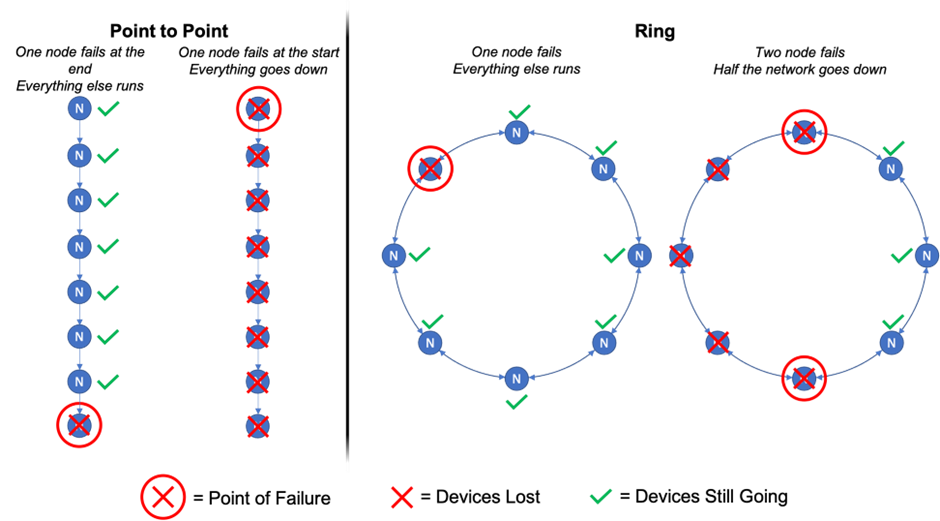
\includegraphics[width=1\linewidth]{Images/bad_topologies.png}
            \caption{Point-to-Point and Ring Topology}
            \label{fig:bad_topologies}
        \end{figure}

        \begin{figure}[H]
            \centering
            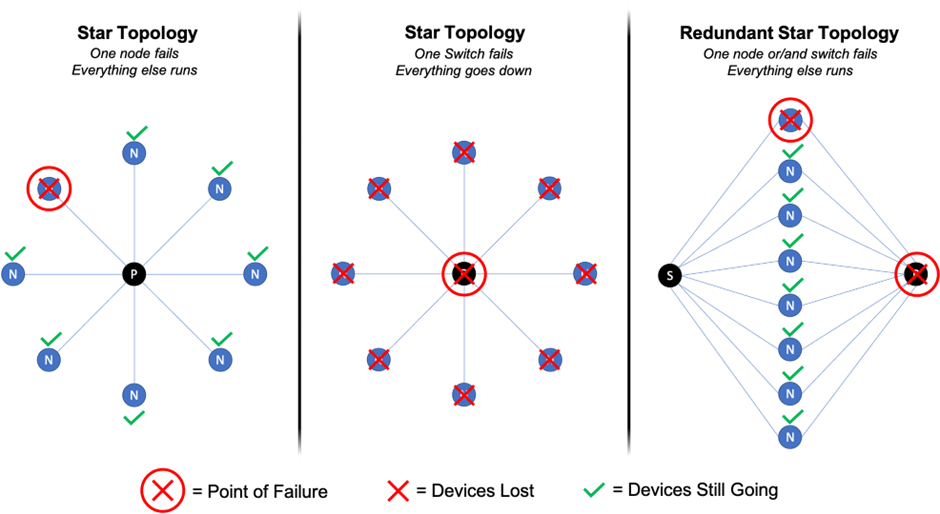
\includegraphics[width=1\linewidth]{Images/redundant_star_topology.png}
            \caption{Start and Redundant Star Topology}
            \label{fig:redundant_star_topology}
        \end{figure}
        
        The system integration plan below shows the \gls{foh} connections on the left and the stage connections on the right (Figure \ref{fig:system_integration_plan}). iPads can also be used with a \gls{wap} to control either console remotely using the SD-Core 2 app.
        
        \begin{figure}[H]
            \centering
            \includegraphics[width=1\linewidth]{Images/system_integration_plan.png}
            \caption{System Integration Plan (Light Blue: Primary Dante, Red: Secondary Dante, Yellow: OPTO, Dark Blue: SoundGrid, Purple: AES3, Green: AES80/OCA, Black: Standard Ethernet)}
            \label{fig:system_integration_plan}
        \end{figure}

        The amplifier configurations are provided at \ref{appendix:speaker_amp_config} and the full patch sheet for the sound system is displayed at \ref{appendix:speaker_patch}; showing the routing between the network bridges, signal engine, amplifiers, and speakers.

        \subsubsection{Audio Networking}
            The choice of the audio networking protocol for this event is primarily influenced by its popularity and compatibility with an extensive list of products (Figure \ref{fig:audio_networking_protocols}).

            \begin{figure}[H]
                \centering
                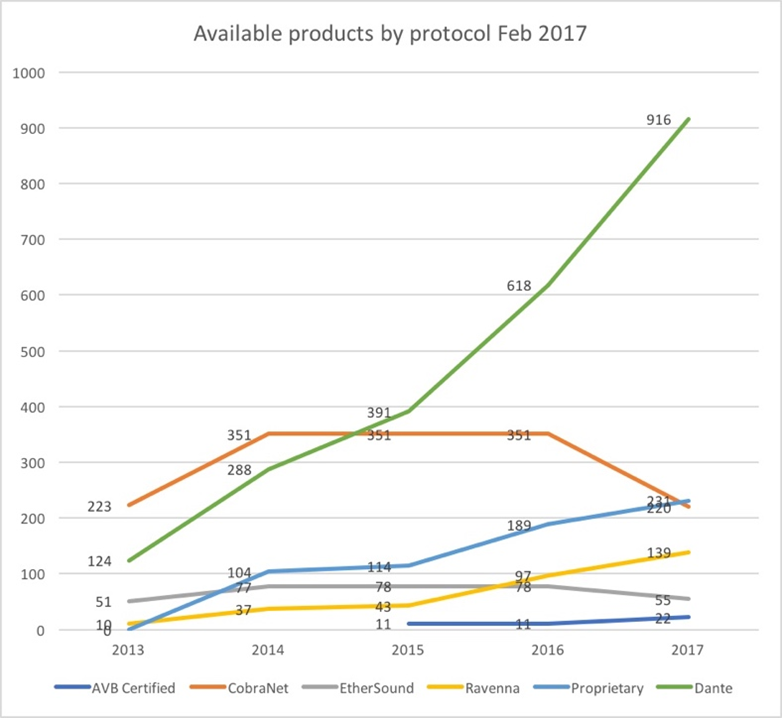
\includegraphics[width=0.8\linewidth]{Images/audio_networking_protocols.png}
                \caption{Popularity of Audio Networking Protocols}
                \label{fig:audio_networking_protocols}
            \end{figure}
            
            Dante enables Audio over IP, allowing seamless communication among compatible devices without requiring specific switches or cables—just a standard Ethernet (CAT5 or higher). Dante is an industry standard, offering expandability for audio, video, and lighting with many topology options such as the redundant star. It has user-friendly 'plug and play' features (making implementation easier) such as automatic device discovery and IP assignment through DHCP in Dante Controller, and automatic master clock assignment. Table \ref{tab:networking_protocol_comparison} shows comparisons of other networks that were also explored.
            
            \begin{longtable}[H]{|p{2cm}|
                >{\columncolor[HTML]{9AFF99}}p{6.8cm} |
                >{\columncolor[HTML]{FFCCC9}}p{6.8cm} |}
                \hline
                 &
                  \textbf{Pros} &
                  \textbf{Cons} \\ \hline
                \endfirsthead
                %
                \endhead
                %
                \textbf{Dante} &
                  One of the most popular protocols in the industry with low latency and high quality audio. Requires standard Ethernet cables. Integrates with AES67. Scalable for all applications with a complete networking solution. 'Plug and play' with automatic device discovery and master clock assignment. Provides audio, video and lighting / DMX control. Any L2 or IP network topology can be used. Integrates well with many products including d7b audiotechnik. &
                  Proprietary software which is expensive due to licensing and requires a few hours of training to understand the technology. Requires dedicated Dante enabled devices. \\ \hline
                \textbf{SoundGrid} &
                  Provides plugin processing, offload \gls{dsp} to remote servers. Integration with waves plugins. Compatible with most of the DiGiCo SD range. &
                  Proprietary software and hardware which is expensive as licensing is required for each server. Waves hardware is quite costly and not many companies provide waves as a standard networking protocol by default. Only allows for Star and daisy chain topologies. Only allows for 3 hops until higher latency starts to occur. \\ \hline
                \textbf{MADI} &
                  Easy to setup and quite reliable and robust. Allows for long cable runs with little signal loss. Cost-effective and is used widely on various Soundcraft and DiGiCo products. &
                  Limited bandwidth for high channel counts. Requires Point-to-point connections with no redundancy. Lack of advanced features compared to IP protocols. \\ \hline
                \textbf{AES50} &
                  Part of the AES standard and is widely used on various Midas and Behringer products. Provides better channel count capability than AES3, ADAT and TDIF with low latency. Reliable with support for long cable runs and well suited for medium sized applications. Easy to install and understand &
                  Only allows for Point-to-Point topology and limited interoperability with other protocols \\ \hline
                \textbf{AVB} &
                  IEEE standard for audio and video. Quality of Service (QoS) support and great with time sensitive applications. Scalable for various network sizes and low latency. Integrates well with L'Acoustics products. Open Source format so a lower cost. &
                  Not as popular as Dante in the industry and requires proprietary networking equipment. Only allows spanning tree topology \\ \hline
                  \caption{Networking Protocol Comparison}
                  \label{tab:networking_protocol_comparison}
            \end{longtable}

            
            \subsubsection{Full Equipment List}
                \begin{longtable}[H]{|p{3cm}|p{4cm}|p{2cm}|p{3cm}|p{2cm}|}
                \hline
\textbf{Type} & \textbf{Item} & \textbf{Price (inc VAT)} & \textbf{Quantity} & \textbf{Total Price} \\ \hline
\endfirsthead
%
\endhead
%
\rowcolor[HTML]{EFEFEF} 
FOH \& MON Console                 & SD12                               & \cellcolor[HTML]{EFEFEF}£300* & 2                                  & £600   \\ \hline
Stagebox                           & SD-Rack                            & £80*                          & 1                                  & £80    \\ \hline
\rowcolor[HTML]{EFEFEF} 
License                            & SuperRack License                  & \cellcolor[HTML]{EFEFEF}£471  & 1 (optional)                       & £471   \\ \hline
\rowcolor[HTML]{EFEFEF} 
License                            & Dante License                      & \cellcolor[HTML]{EFEFEF}£15   & 2                                  & £30    \\ \hline
\rowcolor[HTML]{EFEFEF} 
License                            & G and GB RF License                & \cellcolor[HTML]{EFEFEF}£85   & 1                                  & £85    \\ \hline
Expansion Card                     & DMI-DANTE64@96                     & £1586                         & 3                                  & £4758  \\ \hline
Expansion Card                     & DMI-WAVES                          & £931                          & 1 (optional)                       & £931   \\ \hline
\rowcolor[HTML]{EFEFEF} 
DSP Server                         & ONE-C Server                       & £200*                         & 1 (optional)                       & £200   \\ \hline
Bridge                             & Orange Box                         & £1188                         & 1                                  & £1188  \\ \hline
Bridge                             & DS10                               & £30*                          & 6                                  & £180   \\ \hline
\rowcolor[HTML]{EFEFEF} 
DSP Engine                         & DS100                              & £196*                         & 1 (optional)                       & £196   \\ \hline
Amplifier                          & D80                                & £70*                          & 44                                 & £3080  \\ \hline
Amplifier                          & D40                                & £60*                          & 12                                 & £720   \\ \hline
Amplifier                          & D20                                & £50*                          & 5                                  & £250   \\ \hline
\rowcolor[HTML]{EFEFEF} 
Speaker                            & GSL12                              & £70*                          & 76                                 & £5320  \\ \hline
\rowcolor[HTML]{EFEFEF} 
Speaker                            & KSL-SUB                            & £75*                          & 8                                  & £600   \\ \hline
\rowcolor[HTML]{EFEFEF} 
Speaker                            & KSL12                              & £65*                          & 28                                 & £1820  \\ \hline
\rowcolor[HTML]{EFEFEF} 
Speaker                            & SL-SUB                             & £80*                          & 12                                 & £960   \\ \hline
\rowcolor[HTML]{EFEFEF} 
Speaker                            & V8                                 & £40*                          & 6                                  & £240   \\ \hline
\rowcolor[HTML]{EFEFEF} 
Speaker                            & V-SUB                              & £30*                          & 2                                  & £60    \\ \hline
\rowcolor[HTML]{EFEFEF} 
Speaker                            & Y10P                               & £35*                          & 4                                  & £140   \\ \hline
Rigging                            & GSL Compression set                & £15*                          & 2                                  & £30    \\ \hline
Rigging                            & Hoist chain 4t                     & £15*                          & 12 (only 10 if using aiming plate) & £180   \\ \hline
Rigging                            & SL Aiming plate                    & £15*                          & 6 (optional)                       & £90    \\ \hline
Rigging                            & GSL Flying frame set               & £15*                          & 4                                  & £60    \\ \hline
Rigging                            & KSL Flying frame set               & £15*                          & 2                                  & £30    \\ \hline
Rigging                            & KSL Compression set                & £15*                          & 2                                  & £30    \\ \hline
Rigging                            & KSL-SUB Adapter frame              & £15*                          & 2                                  & £30    \\ \hline
Rigging                            & V Flying frame                     & £15*                          & 2                                  & £30    \\ \hline
\rowcolor[HTML]{EFEFEF} 
\gls{iem} Transmitter Set     & Sennheiser SR2050                  & £3499                         & 5                                  & £17495 \\ \hline
\rowcolor[HTML]{EFEFEF} 
\gls{iem} pack                & Sennheiser EM2050                  & -                             & 20 (4 per bundle)                  & -      \\ \hline
\rowcolor[HTML]{EFEFEF} 
\gls{iem} battery charger     & Sennheiser BA 2-way Charger        & £182                          & 2                                  & £364   \\ \hline
\rowcolor[HTML]{EFEFEF} 
\gls{iem} spare batteries     & Sennheiser BA 2015                 & £50                           & 8                                  & £400   \\ \hline
\rowcolor[HTML]{EFEFEF} 
\gls{iem} Antenna Combiner    & Shure PA821B                       & £3110                         & 2                                  & £6220  \\ \hline
\rowcolor[HTML]{EFEFEF} 
\gls{iem} Antenna             & Sennheiser A5000                   & £829                          & 2                                  & £1658  \\ \hline
\rowcolor[HTML]{EFEFEF} 
\gls{iem} Antenna Cable       & \SI{5}{\metre} N-Type Cable        & £20                           & 2                                  & £40    \\ \hline
\rowcolor[HTML]{EFEFEF} 
\gls{iem} Antenna Cable       & \SI{10}{\metre} N-Type Cable       & £50                           & 2                                  & £100   \\ \hline
Hardware                           & Limiter Empirical Labs EL7X Fatso  & £2449                         & 2                                  & £4898  \\ \hline
Hardware                           & TC Electronic Reverb 4000          & £764                          & 2                                  & £1528  \\ \hline
Hardware                           & Waves Maxx BCL Digital Compressor  & £1883                         & 1                                  & £1883  \\ \hline
\rowcolor[HTML]{EFEFEF} 
Switch                             & Cisco SG350-10MP                   & £250                          & 4                                  & £1000  \\ \hline
\rowcolor[HTML]{EFEFEF} 
Switch                             & Cisco SG250-08                     & £108                          & 1                                  & £108   \\ \hline
\rowcolor[HTML]{EFEFEF} 
\gls{wap}                     & Cisco Catalyst 9100 \gls{wap} & £300                          & 2 (optional)                       & £600   \\ \hline
Tablet                             & iPad                               & £326                          & 2 (optional)                       & £652   \\ \hline
Computer                           & MacBook Pro                        & £1699                         & 2 (+1 optional)                    & £5097  \\ \hline
\rowcolor[HTML]{EFEFEF} 
Microphone                         & Sennheiser MKH 416-P48U3           & £695                          & 2                                  & £1390  \\ \hline
\rowcolor[HTML]{EFEFEF} 
\cellcolor[HTML]{EFEFEF}Microphone & DPA4090                            & £899                          & 2                                  & £1798  \\ \hline
\rowcolor[HTML]{EFEFEF} 
\cellcolor[HTML]{EFEFEF}Microphone & Shure Beta 91A                     & £279                          & 1                                  & £279   \\ \hline
\rowcolor[HTML]{EFEFEF} 
\cellcolor[HTML]{EFEFEF}Microphone & Shure Beta 52A                     & £165                          & 1                                  & £165   \\ \hline
\rowcolor[HTML]{EFEFEF} 
\cellcolor[HTML]{EFEFEF}Microphone & Sennheiser e904                    & £155                          & 2                                  & £310   \\ \hline
\rowcolor[HTML]{EFEFEF} 
\cellcolor[HTML]{EFEFEF}Microphone & Beyerdynamic M201TG                & £303                          & 2                                  & £606   \\ \hline
\rowcolor[HTML]{EFEFEF} 
\cellcolor[HTML]{EFEFEF}Microphone & Sennheiser e604                    & £144                          & 1                                  & £144   \\ \hline
\rowcolor[HTML]{EFEFEF} 
\cellcolor[HTML]{EFEFEF}Microphone & Audix D4                           & £152                          & 2                                  & £304   \\ \hline
\rowcolor[HTML]{EFEFEF} 
\cellcolor[HTML]{EFEFEF}Microphone & Shure SM81                         & £338                          & 2                                  & £676   \\ \hline
\rowcolor[HTML]{EFEFEF} 
\cellcolor[HTML]{EFEFEF}Microphone & Shure KSM141                       & £341                          & 2                                  & £682   \\ \hline
\rowcolor[HTML]{EFEFEF} 
\cellcolor[HTML]{EFEFEF}Microphone & Sennheiser e609                    & £96                           & 3                                  & £288   \\ \hline
\rowcolor[HTML]{EFEFEF} 
\cellcolor[HTML]{EFEFEF}Microphone & SE8                                & £151                          & 4                                  & £604   \\ \hline
\rowcolor[HTML]{EFEFEF} 
\cellcolor[HTML]{EFEFEF}Microphone & Sennheiser e945                    & £163                          & 2                                  & £326   \\ \hline
\rowcolor[HTML]{EFEFEF} 
\cellcolor[HTML]{EFEFEF}DI         & Mackie MDB-1P                      & £43                           & 10                                 & £430   \\ \hline
\rowcolor[HTML]{EFEFEF} 
\cellcolor[HTML]{EFEFEF}DI         & Mackie MDB-2P                      & £63                           & 2                                  & £126   \\ \hline
\rowcolor[HTML]{EFEFEF} 
Microphone                         & Shure SM57                         & £104                          & 8                                  & £832   \\ \hline
Wireless Microphone Set            & Sennheiser ew 500 G4               & £892                          & 4                                  & £3568  \\ \hline
Wireless Microphone                & Sennheiser SKM 500 G4              & -                             & 4 (1 per bundle)                   &        \\ \hline
\rowcolor[HTML]{EFEFEF} 
Tall Stand                         & K\&M 20800                          & £77                           & 2                                  & £154   \\ \hline
\rowcolor[HTML]{EFEFEF} 
Standard Stand                     & K\&M 2102                           & £63                           & 23                                 & £1449  \\ \hline
\rowcolor[HTML]{EFEFEF} 
Short Stand                        & K\&M 25905                          & £33                           & 5                                  & £165   \\ \hline
Generator (1250 kVA)        &                &      £1750    &        1           &    £1750    \\ \hline
                    \caption{Full Equipment List (*day rental)}
                    \label{tab:full_equipment_list}
                \end{longtable}